\documentclass[10pt,dvips,openbib]{article}
\usepackage{makeidx}
\usepackage[all,web,line,arc,tile,color]{xy}
\usepackage[plainpages=false,pdfpagelabels,breaklinks,pagebackref]{hyperref}
\usepackage{mydefs}
\usepackage{algorithm}        % after hyperref
\usepackage{chicago}
\usepackage{glosstex}
\usepackage{newproof}

\makeglossary
\makeindex

\newdimen\intercol

\begin{document}

\title{\barvinok/: User Guide\\
\small Version: \input{version} }
\author{Sven Verdoolaege}

\maketitle

\addcontentsline{toc}{section}{\contentsname}
\tableofcontents

\listoffigures

\section{Internal Representation of the \protect\ai[\tt]{barvinok} library}

Our \barvinok/ library is built on top of \PolyLib/ 
\shortcite{Wilde1993,Loechner1999}.
In particular, it reuses the implementations
of the algorithm of 
\shortciteN{Loechner97parameterized}
for computing parametric vertices
and the algorithm of
\shortciteN{Clauss1998parametric}
for computing chamber decompositions.
Initially, our library was meant to be a replacement
for the algorithm of \shortciteN{Clauss1998parametric},
also implemented in \PolyLib/, for computing quasi-polynomials.
To ease the transition of application programs we
tried to reuse the existing data structures as much as possible.

\subsection{Existing Data Structures}
\label{a:existing}

Inside \PolyLib/ integer values are represented by the 
\ai[\tt]{Value} data type.
Depending on a configure option, the data type may
either by a 32-bit integer, a 64-bit integer
or an arbitrary precision integer using \ai[\tt]{GMP}.
The \barvinok/ library requires that \PolyLib/ is compiled
with support for arbitrary precision integers.

The basic structure for representing (unions of) polyhedra is a
\ai[\tt]{Polyhedron}.
\begin{verbatim}
typedef struct polyhedron {
  unsigned Dimension, NbConstraints, NbRays, NbEq, NbBid;
  Value **Constraint;
  Value **Ray;
  Value *p_Init;
  int p_Init_size;
  struct polyhedron *next;
} Polyhedron;
\end{verbatim}
The attribute \ai[\tt]{Dimension} is the dimension
of the ambient space, i.e., the number of variables.
The attributes \ai[\tt]{Constraint}
and \ai[\tt]{Ray} point to two-dimensional arrays
of constraints and generators, respectively.
The number of rows is stored in
\ai[\tt]{NbConstraints} and
\ai[\tt]{NbRays}, respectively.
The number of columns in both arrays is equal
to \verb!1+Dimension+1!.
The first column of \ai[\tt]{Constraint} is either
$0$ or $1$ depending on whether the constraint 
is an equality ($0$) or an inequality ($1$).
The number of equalities is stored in \ai[\tt]{NbEq}.
If the constraint is $\sp a x + c \ge 0$, then
the next columns contain the coefficients $a_i$
and the final column contains the constant $c$.
The first column of \ai[\tt]{Ray} is either
$0$ or $1$ depending on whether the generator 
is a line ($0$) or a vertex or ray ($1$).
The number of lines is stored in \ai[\tt]{NbBid}.
Let $d$ be the \ac{lcm} of the denominators of the coordinates
of a vertex $\vec v$, then the next columns contain
$d v_i$ and the final column contains $d$.
For a ray, the final column contains $0$.
The field \ai[\tt]{next} points to the next polyhedron in
the union of polyhedra.
It is \verb+0+ if this is the last (or only) polyhedron in the union.
For more information on this structure, we refer to \shortciteN{Wilde1993}.

Quasi-polynomials are represented using the 
\ai[\tt]{evalue} and \ai[\tt]{enode} structures.
\begin{verbatim}
typedef enum { polynomial, periodic, evector } enode_type;

typedef struct _evalue {
  Value d;              /* denominator */
  union {
    Value n;            /* numerator (if denominator != 0) */
    struct _enode *p;   /* pointer   (if denominator == 0) */
  } x;
} evalue;

typedef struct _enode {
  enode_type type;      /* polynomial or periodic or evector */
  int size;             /* number of attached pointers */
  int pos;              /* parameter position */
  evalue arr[1];        /* array of rational/pointer */
} enode;
\end{verbatim}
If the field \ai[\tt]{d} of an \ai[\tt]{evalue} is zero, then
the \ai[\tt]{evalue} is a placeholder for a pointer to
an \ai[\tt]{enode}, stored in \ai[\tt]{x.p}.
Otherwise, the \ai[\tt]{evalue} is a rational number with
numerator \ai[\tt]{x.n} and denominator \ai[\tt]{d}.
An \ai[\tt]{enode} is either a \ai[\tt]{polynomial}
or a \ai[\tt]{periodic}, depending on the value
of \ai[\tt]{type}.
The length of the array \ai[\tt]{arr} is stored in \ai[\tt]{size}.
For a \ai[\tt]{polynomial}, \ai[\tt]{arr} contains the coefficients.
For a \ai[\tt]{periodic}, it contains the values for the different
residue classes modulo the parameter indicated by \ai[\tt]{pos}.
For a polynomial, \ai[\tt]{pos} refers to the variable
of the polynomial.
The value of \ai[\tt]{pos} is \verb+1+ for the first parameter.
That is, if the value of \ai[\tt]{pos} is \verb+1+ and the first
parameter is $p$, and if the length of the array is $l$,
then in case it is a polynomial, the
 \ai[\tt]{enode} represents
$$
\verb+arr[0]+ + \verb+arr[1]+ p + \verb+arr[2]+ p^2 + \cdots +
\verb+arr[l-1]+ p^{l-1}
.
$$
If it is a periodic, then it represents
$$
\left[
\verb+arr[0]+, \verb+arr[1]+,  \verb+arr[2]+, \ldots,
\verb+arr[l-1]+
\right]_p
.
$$
Note that the elements of a \ai[\tt]{periodic} may themselves
be other \ai[\tt]{periodic}s or even \ai[\tt]{polynomial}s.
In our library, we only allow the elements of a  \ai[\tt]{periodic}
to be other \ai[\tt]{periodic}s or rational numbers.
The chambers and their corresponding quasi-polynomial are
stored in \ai[\tt]{Enumeration} structures.
\begin{verbatim}
typedef struct _enumeration {
  Polyhedron *ValidityDomain; /* constraints on the parameters */
  evalue EP;                  /* dimension = combined space    */
  struct _enumeration *next;  /* Ehrhart Polynomial,
                                 corresponding to parameter
                                 values inside the domain
                                 ValidityDomain above          */
} Enumeration;
\end{verbatim}
For more information on these structures, we refer to \shortciteN{Loechner1999}.

\begin{example}
Figure~\ref{f:Loechner} is a skillful reconstruction
of Figure~2 from \shortciteN{Loechner1999}.
It shows the contents of the \ai[\tt]{enode} structures
representing the quasi-polynomial
$
[1,2]_p p^2 + 3 p + \frac 5 2
$.

\begin{figure}
\begin{xy}
\POS(0,0)*!UL{\hbox{
\tt
\begin{tabular}{|c|c|c|}
\hline
\multicolumn{2}{|c|}{type} & polynomial \\
\hline
\multicolumn{2}{|c|}{size} & 3 \\
\hline
\multicolumn{2}{|c|}{pos} & 1 \\
\hline
\smash{\lower 6.25pt\hbox{arr[0]}} & d & 2 \\
\cline{2-3}
       & x.n & 5 \\
\hline
\smash{\lower 6.25pt\hbox{arr[1]}} & d & 1 \\
\cline{2-3}
       & x.n & 3 \\
\hline
\smash{\lower 6.25pt\hbox{arr[2]}} & d & 0 \\
\cline{2-3}
       & x.p &   \\
\hline
\end{tabular}
}
}="box1"
+DR*!DR\hbox{\strut\hskip 1.5\tabcolsep\phantom{\tt polynomial}\hskip 1.5\tabcolsep}+C="a"
\POS(60,-15)*!UL{\hbox{
\tt
\begin{tabular}{|c|c|c|}
\hline
\multicolumn{2}{|c|}{type} & periodic \\
\hline
\multicolumn{2}{|c|}{size} & 2 \\
\hline
\multicolumn{2}{|c|}{pos} & 1 \\
\hline
\smash{\lower 6.25pt\hbox{arr[0]}} & d & 1 \\
\cline{2-3}
       & x.n & 1 \\
\hline
\smash{\lower 6.25pt\hbox{arr[1]}} & d & 1 \\
\cline{2-3}
       & x.n & 2 \\
\hline
\end{tabular}
}
}="box2"
+UL+<0.5\tabcolsep,0pt>*!UL\hbox{\strut}+CL="b"
\POS"a"\ar@(r,l) "b"
\POS"box1"+UC*++!D\hbox{\tt enode}
\POS"box2"+UC*++!D\hbox{\tt enode}
\end{xy}
\caption{The quasi-polynomial $[1,2]_p p^2 + 3 p + \frac 5 2$.}
\label{f:Loechner}
\end{figure}
\end{example}

\subsection{Options}
\label{a:options}

The \ai[\tt]{barvinok\_options} structure contains various
options that influence the behavior of the library.

\begin{verbatim}
struct barvinok_options {
    /* PolyLib options */
    unsigned    MaxRays;

    /* NTL options */
                /* LLL reduction parameter delta=LLL_a/LLL_b */
    long        LLL_a;
    long        LLL_b;

    /* barvinok options */
                /*
                 * 0: no
                 * 1: depth first
                 * 2: breadth frist
                 */
    int         incremental_specialization;
};

struct barvinok_options *barvinok_options_new_with_defaults();
\end{verbatim}

The function \ai[\tt]{barvinok\_options\_new\_with\_defaults}
can be used to create a \ai[\tt]{barvinok\_options} structure
with default values.

\begin{itemize}
\item \PolyLib/ options

\begin{itemize}

\item \ai[\tt]{MaxRays}

The value of \ai[\tt]{MaxRays} is passed to various \PolyLib/
functions and defines the
maximum size of a table used in the \ai{double description} computation
in the \PolyLib/ function \ai[\tt]{Chernikova}.
In earlier versions of \PolyLib/,
this parameter had to be conservatively set
to a high number to ensure successful operation,
resulting in significant memory overhead.
Our change to allow this table to grow
dynamically is available in recent versions of \PolyLib/.
In these versions, the value no longer indicates the maximal
table size, but rather the size of the initial allocation.
This value may be set to \verb+0+ or left as set
by \ai[\tt]{barvinok\_options\_new\_with\_defaults}.

\end{itemize}

\item \ai[\tt]{NTL} options

\begin{itemize}

\item \ai[\tt]{LLL\_a}
\item \ai[\tt]{LLL\_b}

The values used for the \ai{reduction parameter}
in the call to \ai[\tt]{NTL}'s implemenation of \indac{LLL}.

\end{itemize}

\item \ai[\tt]{barvinok} specific options

\begin{itemize}

\item \ai[\tt]{incremental\_specialization}

Selects the \ai{specialization} algorithm to be used.
If set to {\tt 0} then a direct specialization is performed
using a random vector.
Value {\tt 1} selects a depth first incremental specialization,
while value {\tt 2} selects a breadth first incremental specialization.
The default is selected by the \ai[\tt]{--enable-incremental}
\ai[\tt]{configure} option.
For more information we refer to~\citeN[Section~4.4.3]{Verdoolaege2005PhD}.

\end{itemize}

\end{itemize}

\subsection{Data Structures for Quasi-polynomials}
\label{a:data}

Internally, we do not represent our quasi-polynomials
as step-polynomials, but, similarly to \shortciteN{Loechner1999},
as polynomials with periodic numbers for coefficients.
However, we also allow our periodic numbers to be represented by
fractional parts of degree-$1$ polynomials rather than
an explicit enumeration using the \ai[\tt]{periodic} type.
By default, the current version of \barvinok/ uses
\ai[\tt]{periodic}s, but this can be changed through
the \ai[\tt]{--enable-fractional} configure option.
In the latter case, the quasi-polynomial using fractional
parts can also be converted to an actual step-polynomial
using \ai[\tt]{evalue\_frac2floor}, but this is not fully
supported yet.

For reasons of compatibility,%
\footnote{Also known as laziness.}
we shoehorned our representations for piecewise quasi-polynomials
into the existing data structures.
To this effect, we introduced four new types,
\ai[\tt]{fractional}, \ai[\tt]{relation},
\ai[\tt]{partition} and \ai[\tt]{flooring}.
\begin{verbatim}
typedef enum { polynomial, periodic, evector, fractional,
               relation, partition, flooring } enode_type;
\end{verbatim}
The field \ai[\tt]{pos} is not used in most of these
additional types and is therefore set to \verb+-1+.

The types \ai[\tt]{fractional} and \ai[\tt]{flooring}
represent polynomial expressions in a fractional part or a floor respectively.
The generator is stored in \verb+arr[0]+, while the
coefficients are stored in the remaining array elements.
That is, an \ai[\tt]{enode} of type \ai[\tt]{fractional}
represents
$$
\verb+arr[1]+ + \verb+arr[2]+ \{\verb+arr[0]+\} + 
\verb+arr[3]+ \{\verb+arr[0]+\}^2 + \cdots +
\verb+arr[l-1]+ \{\verb+arr[0]+\}^{l-2}
.
$$
An \ai[\tt]{enode} of type \ai[\tt]{flooring}
represents
$$
\verb+arr[1]+ + \verb+arr[2]+ \lfloor\verb+arr[0]+\rfloor + 
\verb+arr[3]+ \lfloor\verb+arr[0]+\rfloor^2 + \cdots +
\verb+arr[l-1]+ \lfloor\verb+arr[0]+\rfloor^{l-2}
.
$$

\begin{example}
The internal representation of the quasi-polynomial
$$\left(1+2 \left\{\frac p 2\right\}\right) p^2 + 3 p + \frac 5 2$$
is shown in Figure~\ref{f:fractional}.

\begin{figure}
\begin{xy}
\POS(0,0)*!UL{\hbox{
\tt
\begin{tabular}{|c|c|c|}
\hline
\multicolumn{2}{|c|}{type} & polynomial \\
\hline
\multicolumn{2}{|c|}{size} & 3 \\
\hline
\multicolumn{2}{|c|}{pos} & 1 \\
\hline
\smash{\lower 6.25pt\hbox{arr[0]}} & d & 2 \\
\cline{2-3}
       & x.n & 5 \\
\hline
\smash{\lower 6.25pt\hbox{arr[1]}} & d & 1 \\
\cline{2-3}
       & x.n & 3 \\
\hline
\smash{\lower 6.25pt\hbox{arr[2]}} & d & 0 \\
\cline{2-3}
       & x.p &   \\
\hline
\end{tabular}
}
}="box1"
+DR*!DR\hbox{\strut\hskip 1.5\tabcolsep\phantom{\tt polynomial}\hskip 1.5\tabcolsep}+C="a"
\POS(60,0)*!UL{\hbox{
\tt
\begin{tabular}{|c|c|c|}
\hline
\multicolumn{2}{|c|}{type} & fractional \\
\hline
\multicolumn{2}{|c|}{size} & 3 \\
\hline
\multicolumn{2}{|c|}{pos} & -1 \\
\hline
\smash{\lower 6.25pt\hbox{arr[0]}} & d & 0 \\
\cline{2-3}
       & x.p &   \\
\hline
\smash{\lower 6.25pt\hbox{arr[1]}} & d & 1 \\
\cline{2-3}
       & x.n & 1 \\
\hline
\smash{\lower 6.25pt\hbox{arr[2]}} & d & 1 \\
\cline{2-3}
       & x.n & 2 \\
\hline
\end{tabular}
}
}="box2"
+UL+<0.5\tabcolsep,0pt>*!UL\hbox{\strut}+CL="b"
\POS"a"\ar@(r,l) "b"
\POS"box2"+UR*!UR{\hbox{
\tt
\begin{tabular}{|c|}
\hline
 fractional \\
\hline
 3 \\
\hline
 -1 \\
\hline
 0 \\
\hline
\end{tabular}
}
}+CD*!U{\strut}+C="c"
\POS(60,-50)*!UL{\hbox{
\tt
\begin{tabular}{|c|c|c|}
\hline
\multicolumn{2}{|c|}{type} & polynomial \\
\hline
\multicolumn{2}{|c|}{size} & 2 \\
\hline
\multicolumn{2}{|c|}{pos} & 1 \\
\hline
\smash{\lower 6.25pt\hbox{arr[0]}} & d & 1 \\
\cline{2-3}
       & x.n & 0 \\
\hline
\smash{\lower 6.25pt\hbox{arr[1]}} & d & 2 \\
\cline{2-3}
       & x.n & 1 \\
\hline
\end{tabular}
}
}="box3"
+UR-<0.8\tabcolsep,0pt>*!UR\hbox{\strut}+CR="d"
\POS"c"\ar@(r,r) "d"
\POS"box1"+UC*++!D\hbox{\tt enode}
\POS"box2"+UC*++!D\hbox{\tt enode}
\POS"box3"+UC*++!D\hbox{\tt enode}
\end{xy}
\caption{The quasi-polynomial 
$\left(1+2 \left\{\frac p 2\right\}\right) p^2 + 3 p + \frac 5 2$.}
\label{f:fractional}
\end{figure}

\end{example}

The \ai[\tt]{relation} type is used to represent \ai{stride}s.
In particular, if the value of \ai[\tt]{size} is 2, then
the value of a \ai[\tt]{relation} is (in pseudo-code):
\begin{verbatim}
(value(arr[0]) == 0) ? value(arr[1]) : 0
\end{verbatim}
If the size is 3, then the value is:
\begin{verbatim}
(value(arr[0]) == 0) ? value(arr[1]) : value(arr[2])
\end{verbatim}
The type of \verb+arr[0]+ is typically \ai[\tt]{fractional}.

Finally, the \ai[\tt]{partition} type is used to
represent piecewise quasi-polynomials.
We prefer to encode this information inside \ai[\tt]{evalue}s
themselves
rather than using \ai[\tt]{Enumeration}s since we want
to perform the same kinds of operations on both quasi-polynomials
and piecewise quasi-polynomials.
An \ai[\tt]{enode} of type \ai[\tt]{partition} may not be nested
inside another \ai[\tt]{enode}.
The size of the array is twice the number of ``chambers''.
Pointers to chambers are stored in the even slots,
whereas pointer to the associated quasi-polynomials
are stored in the odd slots.
To be able to store pointers to chambers, the
definition of \ai[\tt]{evalue} was changed as follows.
\begin{verbatim}
typedef struct _evalue {
  Value d;              /* denominator */
  union {
    Value n;            /* numerator (if denominator > 0) */
    struct _enode *p;   /* pointer   (if denominator == 0) */
    Polyhedron *D;      /* domain    (if denominator == -1) */
  } x;
} evalue;
\end{verbatim}
Note that we allow a ``chamber'' to be a union of polyhedra
as discussed in \citeN[Section~4.5.1]{Verdoolaege2005PhD}.
Chambers with extra variables, i.e., those of
\citeN[Section~4.6.5]{Verdoolaege2005PhD},
are only partially supported.
The field \ai[\tt]{pos} is set to the actual dimension,
i.e., the number of parameters.

\subsection{Operations on Quasi-polynomials}
\label{a:operations}

In this section we discuss some of the more important
operations on \ai[\tt]{evalue}s provided by the
\barvinok/ library.
Some of these operations are extensions
of the functions from \PolyLib/ with the same name.

\begin{verbatim}
void eadd(evalue *e1,evalue *res);
void emul (evalue *e1, evalue *res );
\end{verbatim}
The functions \ai[\tt]{eadd} and \ai[\tt]{emul} takes
two (pointers to) \ai[\tt]{evalue}s \verb+e1+ and \verb+res+
and computes their sum and product respectively.
The result is stored in \verb+res+, overwriting (and deallocating)
the original value of \verb+res+.
It is an error if exactly one of
the arguments of \ai[\tt]{eadd} is of type \ai[\tt]{partition}
(unless the other argument is \verb+0+).
The addition and multiplication operations are described
in \citeN[Section~4.5.1]{Verdoolaege2005PhD} 
and~\citeN[Section~4.5.2]{Verdoolaege2005PhD}
respectively.

The function \ai[\tt]{eadd} is an extension of the function
\ai[\tt]{new\_eadd} from \shortciteN{Seghir2002}.
Apart from supporting the additional types from Section~\ref{a:data},
the new version also additionally imposes an order on the nesting of
different \ai[\tt]{enode}s.
Without such an ordering, \ai[\tt]{evalue}s could be constructed
representing for example
$$
(0 y^ 0 + ( 0 x^0 + 1 x^1 ) y^1 ) x^0 + (0 y^0 - 1 y^1) x^1
,
$$
which is just a funny way of saying $0$.

\begin{verbatim}
void eor(evalue *e1, evalue *res);
\end{verbatim}
The function \ai[\tt]{eor} implements the \ai{union}
operation from \citeN[Section~4.5.3]{Verdoolaege2005PhD}.  Both arguments
are assumed to correspond to indicator functions.

\begin{verbatim}
evalue *esum(evalue *E, int nvar);
\end{verbatim}
The function \ai[\tt]{esum} performs the summation
operation from \citeN[Section~4.5.4]{Verdoolaege2005PhD}.
The piecewise step-polynomial represented by \verb+E+ is summated
over its first \verb+nvar+ variables.
Note that \verb+E+ must be zero or of type \ai[\tt]{partition}.
The function returns the result in a newly allocated 
\ai[\tt]{evalue}.
Note also that \verb+E+ needs to have been converted
from \ai[\tt]{fractional}s to \ai[\tt]{flooring}s using
the function \ai[\tt]{evalue\_frac2floor}.
\begin{verbatim}
void evalue_frac2floor(evalue *e);
\end{verbatim}
This function also ensures that the arguments of the
\ai[\tt]{flooring}s are positive in the relevant chambers.
It currently assumes that the argument of each
\ai[\tt]{fractional} in the original \ai[\tt]{evalue}
has a minimum in the corresponding chamber.

\begin{verbatim}
double compute_evalue(evalue *e,Value *list_args);
Value *compute_poly(Enumeration *en,Value *list_args);
\end{verbatim}
The functions \ai[\tt]{compute\_evalue} and
\ai[\tt]{compute\_poly} evaluate a (piecewise) quasi-polynomial
at a certain point.  The argument \verb+list_args+
points to an array of \ai[\tt]{Value}s that is assumed
to be long enough.
The \verb+double+ return value of \ai[\tt]{compute\_evalue}
is inherited from \PolyLib/.

\begin{verbatim}
void print_evalue(FILE *DST,evalue *e,char **pname);
\end{verbatim}
The function \ai[\tt]{print\_evalue} dumps a human-readable
representation to the stream pointed to by \verb+DST+.
The argument \verb+pname+ points 
to an array of character strings representing the parameter names.
The array is assumed to be long enough.

\begin{verbatim}
int eequal(evalue *e1,evalue *e2);
\end{verbatim}
The function \ai[\tt]{eequal} return true (\verb+1+) if its
two arguments are structurally identical.
I.e., it does {\em not\/} check whether the two
(piecewise) quasi-polynomial represent the same function.

\begin{verbatim}
void reduce_evalue (evalue *e);
\end{verbatim}
The function \ai[\tt]{reduce\_evalue} performs some
simplifications on \ai[\tt]{evalue}s.
Here, we only describe the simplifications that are directly
related to the internal representation.
Some other simplifications are explained in
\citeN[Section~4.7.2]{Verdoolaege2005PhD}.
If the highest order coefficients of a \ai[\tt]{polynomial},
\ai[\tt]{fractional} or \ai[\tt]{flooring} are zero (possibly
after some other simplifications), then the size of the array
is reduced.  If only the constant term remains, i.e.,
the size is reduced to $1$ for  \ai[\tt]{polynomial} or to $2$
for the other types, then the whole node is replaced by
the constant term.
Additionally, if the argument of a \ai[\tt]{fractional}
has been reduced to a constant, then the whole node
is replaced by its partial evaluation.
A \ai[\tt]{relation} is similarly reduced if its second
branch or both its branches are zero.
Chambers with zero associated quasi-polynomials are
discarded from a \ai[\tt]{partition}.

\subsection{Generating Functions}

The representation of \rgf/s uses 
some basic types from the \ai[\tt]{NTL} library \shortcite{NTL}
for representing arbitrary precision integers
(\ai[\tt]{ZZ}) 
as well as vectors (\ai[\tt]{vec\_ZZ}) and matrices (\ai[\tt]{mat\_ZZ})
of such integers.
Each term in a \rgf/ is represented by a \ai[\tt]{short\_rat}
structure.
\begin{verbatim}
struct short_rat {
    struct {
        /* rows: terms in numerator */
        mat_ZZ  coeff;
        mat_ZZ  power;
    } n;
    struct {
        /* rows: factors in denominator */
        mat_ZZ  power;
    } d;
};
\end{verbatim}
The fields \ai[\tt]{n} and \ai[\tt]{d} represent the
numerator and the denominator respectively.
Note that in our implementation we combine terms
with the same denominator.
In the numerator, each row of \ai[\tt]{coeff} and \ai[\tt]{power}
represents a single such term.
The matrix \ai[\tt]{coeff} has two columns, one for the
numerator and one for the denominator of the rational coefficient
$\alpha_i$ of each term.
The columns of \ai[\tt]{power} correspond to the powers
of the variables.
In the denominator, each row of \ai[\tt]{power}
corresponds to the power $\vec b_{ij}$ of a 
factor in the denominator.

\begin{example}
Figure~\ref{fig:rat}
shows the internal representation of
$$
\frac{\frac 3 2 \, x_0^2 x_1^3 + 2 \, x_0^5 x_1^{-7}}
{ (1 - x_0 x_1^{-3}) (1 - x_1^2)}
.
$$

\begin{figure}
\begin{center}
\begin{minipage}{0cm}
\begin{xy}
*\hbox{
\tt
\begin{tabular}{|c|c|c|}
\hline
n.coeff & 3 & 2 \\
\cline{2-3}
	& 2 & 1 \\
\hline
n.power & 2 & 3 \\
\cline{2-3}
	& 5 & -7 \\
\hline
d.power & 1 & -3 \\
\cline{2-3}
	& 0 & 2 \\
\hline
\end{tabular}
}+UC*++!D\hbox{\tt short\_rat}
\end{xy}
\end{minipage}
\end{center}
\caption{Representation of
$
\left(\frac 3 2 \, x_0^2 x_1^3 + 2 \, x_0^5 x_1^{-7}\right)
/ \left( (1 - x_0 x_1^{-3}) (1 - x_1^2)\right)
$.}
\label{fig:rat}
\end{figure}

\end{example}

The whole \rgf/ is represented by a \ai[\tt]{gen\_fun}
structure.
\begin{verbatim}
struct gen_fun {
    std::vector< short_rat * > term;
    Polyhedron *context;

    void add(ZZ& cn, ZZ& cd, vec_ZZ& num, mat_ZZ& den);
    void print(unsigned int nparam, char **param_name);
    operator evalue *();

    gen_fun(Polyhedron *C = NULL) : context(C) {}
    ~gen_fun();
};
\end{verbatim}
The method \ai[\tt]{gen\_fun::add} adds a new term to the \rgf/.
It makes all powers in the denominator lexico-positive,
orders them in lexicographical order and inserts the new
term in \ai[\tt]{term} according to the lexicographical
order of the combined powers in the denominator.
The method \ai[\tt]{gen\_fun::operator evalue *} performs
the conversion from \rgf/ to \psp/ explained in 
\citeN[Section~4.5.5]{Verdoolaege2005PhD}.
The \ai[\tt]{Polyhedron} \ai[\tt]{context} is the superset
of all points where the enumerator is non-zero used during this conversion,
i.e., it is the set $Q$ from \citeN[Equation~4.31]{Verdoolaege2005PhD}.
If  \ai[\tt]{context} is \verb+NULL+ the maximal
allowed context is assumed, i.e., the maximal
region with lexico-positive rays.  

\subsection{Counting Functions}
\label{a:counting:functions}

Our library provides essentially three different counting functions:
one for non-parametric polytopes, one for parametric polytopes
and one for parametric sets with existential variables.
The old versions of these functions have a ``\ai[\tt]{MaxRays}''
argument, while the new versions have a more general
\ai[\tt]{barvinok\_options} argument.
For more infomation on \ai[\tt]{barvinok\_options}, see Section~\ref{a:options}.

\begin{verbatim}
void barvinok_count(Polyhedron *P, Value* result, 
                    unsigned NbMaxCons);
void barvinok_count_with_options(Polyhedron *P, Value* result,
                                 struct barvinok_options *options);
\end{verbatim}
The function \ai[\tt]{barvinok\_count} or
\ai[\tt]{barvinok\_count\_with\_options} enumerates the non-parametric
polytope \verb+P+ and returns the result in the \ai[\tt]{Value}
pointed to by \verb+result+, which needs to have been allocated
and initialized.
For the meaning of the argument \verb+NbMaxCons+, see
the discussion on \ai[\tt]{MaxRays} in Section~\ref{a:options}.

The function \ai[\tt]{barvinok\_enumerate} for enumerating
parametric polytopes was meant to be
a drop-in replacement of \PolyLib/'s \ai[\tt]{Polyhedron\_Enumerate}
function.
Unfortunately, the latter has been changed to
accept an extra argument in recent versions of \PolyLib/ as shown below.
\begin{verbatim}
Enumeration* barvinok_enumerate(Polyhedron *P, Polyhedron* C, 
                                unsigned MaxRays);
extern Enumeration *Polyhedron_Enumerate(Polyhedron *P,
	    Polyhedron *C, unsigned MAXRAYS, char **pname);
\end{verbatim}
The argument \verb+MaxRays+ has the same meaning as the argument
\verb+NbMaxCons+ above.
The argument \verb+P+ refers to the $(d+n)$-dimensional
polyhedron defining the parametric polytope.
The argument \verb+C+ is an $n$-dimensional polyhedron containing
extra constraints on the parameter space.
Its primary use is to indicate how many of the dimensions
in \verb+P+ refer to parameters as any constraint in \verb+C+
could equally well have been added to \verb+P+ itself.
Note that the dimensions referring to the parameters should
appear {\em last}.
The result is a newly allocated \ai[\tt]{Enumeration}.
As an alternative we also provide a function 
(\ai[\tt]{barvinok\_enumerate\_ev} or
\ai[\tt]{barvinok\_enumerate\_with\_options}) that returns
an \ai[\tt]{evalue}.
\begin{verbatim}
evalue* barvinok_enumerate_ev(Polyhedron *P, Polyhedron* C, 
                              unsigned MaxRays);
evalue* barvinok_enumerate_with_options(Polyhedron *P,
        Polyhedron* C, struct barvinok_options *options);
\end{verbatim}

For enumerating parametric sets with existentially quantified variables,
we provide two functions:
\ai[\tt]{barvinok\_enumerate\_e}
and
\ai[\tt]{barvinok\_enumerate\_pip}.
\begin{verbatim}
evalue* barvinok_enumerate_e(Polyhedron *P,
          unsigned exist, unsigned nparam, unsigned MaxRays);
evalue *barvinok_enumerate_pip(Polyhedron *P,
          unsigned exist, unsigned nparam, unsigned MaxRays);
\end{verbatim}
The first function tries the simplification rules from
\citeN[Section~4.6.2]{Verdoolaege2005PhD} before resorting to the method
based on \indac{PIP} from \citeN[Section~4.6.3]{Verdoolaege2005PhD}.
The second function immediately applies the technique from
\citeN[Section~4.6.3]{Verdoolaege2005PhD}.
The argument \verb+exist+ refers to the number of existential variables,
whereas
the argument \verb+nparam+ refers to the number of parameters.
The order of the dimensions in \verb+P+ is:
counted variables first, then existential variables and finally
the parameters.

The function 
\ai[\tt]{barvinok\_series} or
\ai[\tt]{barvinok\_series\_with\_options} enumerates parametric polytopes
in the form of a \rgf/.
The polyhedron \verb+P+ is assumed to have only
lexico-positive rays.
\begin{verbatim}
gen_fun * barvinok_series(Polyhedron *P, Polyhedron* C, 
                          unsigned MaxRays);
gen_fun * barvinok_series_with_options(Polyhedron *P,
    Polyhedron* C, barvinok_options *options);
\end{verbatim}

\subsection{Auxiliary Functions}

In this section we briefly mention some auxiliary functions
available in the \barvinok/ library.

\begin{verbatim}
void Polyhedron_Polarize(Polyhedron *P);
\end{verbatim}
The function \ai[\tt]{Polyhedron\_Polarize} 
polarizes its argument and is explained
in \citeN[Section~4.4.2]{Verdoolaege2005PhD}.

\begin{verbatim}
Matrix * unimodular_complete(Vector *row);
\end{verbatim}
The function \ai[\tt]{unimodular\_complete} extends
\verb+row+ to a \ai{unimodular matrix} using the
algorithm of \shortciteN{Bik1996PhD}.

\begin{verbatim}
int DomainIncludes(Polyhedron *Pol1, Polyhedron *Pol2);
\end{verbatim}
The function \ai[\tt]{DomainIncludes} extends
the function \ai[\tt]{PolyhedronIncludes}
provided by \PolyLib/ 
to unions of polyhedra.
It checks whether its first argument is a superset of
its second argument.

\begin{verbatim}
Polyhedron *DomainConstraintSimplify(Polyhedron *P, 
                                     unsigned MaxRays);
\end{verbatim}
The value returned by
\ai[\tt]{DomainConstraintSimplify} is a pointer to
a newly allocated \ai[\tt]{Polyhedron} that contains the 
same integer points as its first argument but possibly
has simpler constraints.
Each constraint $ g \sp a x \ge c $
is replaced by $ \sp a x \ge \ceil{ \frac c g } $,
where $g$ is the \ac{gcd} of the coefficients in the original
constraint.
The \ai[\tt]{Polyhedron} pointed to by \verb+P+ is destroyed.

\begin{verbatim}
Polyhedron* Polyhedron_Project(Polyhedron *P, int dim);
\end{verbatim}
The function \ai[\tt]{Polyhedron\_Project} projects
\verb+P+ onto its last \verb+dim+ dimensions.



\section{\texorpdfstring{Applications included
in the \protect\ai[\tt]{barvinok} distribution}
{Applications included in the barvinok distribution}}
\label{a:usage}

\index{barvinok@{\tt  barvinok}!availability}
{\sloppy 
This section describes some application programs
provided by the \barvinok/ library,
available from {\tt http://freshmeat.net/projects/barvinok/.}
For compilation instructions we refer to the \verb+README+ file
included in the distribution.
}

Common option to all programs:\\
\begin{tabular}{lll}
\ai[\tt]{--version} & \ai[\tt]{-V} & print version
\\
\ai[\tt]{--help} & \ai[\tt]{-?} & list available options
\end{tabular}

\subsection{\texorpdfstring{\protect\ai[\tt]{barvinok\_count}}{barvinok\_count}}

The program \ai[\tt]{barvinok\_count} enumerates a
non-parametric polytope.  It takes one polytope
in \PolyLib/ notation as input and prints the number
of integer points in the polytope.
The \PolyLib/ notation corresponds to the internal
representation of \ai[\tt]{Polyhedron}s as explained
in Section~\ref{a:existing}.
\index{input format!constraints}
The first line of the input contains the number of rows
and the number of columns in the \ai[\tt]{Constraint} matrix.
The rest of the input is composed of the elements of the matrix.
Recall that the number of columns is two more than the number
of variables, where the extra first columns is one or zero
depending on whether the constraint is an inequality ($\ge 0$)
or an equality ($= 0$).  The next columns contain
the coefficients of the variables and the final column contains
the constant in the constraint.
E.g., the set 
$S = \lb\, s \mid s \geq 0 \wedge  2 s \leq 13 \, \rb$
from \citeN[Example~38 on page~134]{Verdoolaege2005PhD}
corresponds to the following input and
output.
\begin{verbatim}
> cat S
2 3

1 1 0
1 -2 13
> ./barvinok_count  < S
POLYHEDRON Dimension:1
           Constraints:2  Equations:0  Rays:2  Lines:0
Constraints 2 3
Inequality: [   1   0 ]
Inequality: [  -2  13 ]
Rays 2 3
Vertex: [   0 ]/1
Vertex: [  13 ]/2
   7 
\end{verbatim}
\index{PolyLib@{\tt  PolyLib}!version 5.22.0 or newer}
Note that if you use \PolyLib/ version 5.22.0 or newer then the output
may look slightly different as the computation of the \ai[\tt]{Rays}
may have been postponed to a later stage.
The program \ai[\tt]{latte2polylib.pl} can be used to
convert a polytope from \ai[\tt]{LattE} \shortcite{latte1.1}
notation to \PolyLib/ notation.

\index{input format!vertices}
As an alternative to the constraints based input, the input polytope
may also be specified by its \ai[\tt]{Ray} matrix.
The first line of the input contains the single word \ai[\tt]{vertices}.
The second line contains the number of rows
and the number of columns in the \ai[\tt]{Ray} matrix.
The rest of the input is composed of the elements of the matrix.
Recall that the number of columns is two more than the number
of variables, where the extra first columns is one or zero
depending on whether the ray is a line or not.
The next columns contain
the numerators of the coordinates and the final column contains
the denominator of the vertex or $0$ for a ray.
E.g., the above set can also be described as
\begin{verbatim}
vertices

2 3

1 0 1
1 13 2
\end{verbatim}

\subsection{\texorpdfstring{\protect\ai[\tt]{barvinok\_enumerate}}
{barvinok\_enumerate}}

The program \ai[\tt]{barvinok\_enumerate} enumerates a
parametric polytope as a \psp/ or \rgf/.  It takes two polytopes in \PolyLib/
notation as input, optionally followed by a list of parameter
names.
The two polytopes refer to arguments \verb+P+ and \verb+C+
of the corresponding function. (See Section~\ref{a:counting:functions}.)
The following example was taken by \shortciteN{Loechner1999}
from \shortciteN[Chapter II.2]{Loechner97phd}.
\begin{verbatim}
> cat loechner 
# Dimension of the matrix: 
7 7 
# Constraints: 
# i j k P Q cte 
1 1 0 0 0 0 0 # 0 <= i 
1 -1 0 0 1 0 0 # i <= P 
1 0 1 0 0 0 0 # 0 <= j 
1 1 -1 0 0 0 0 # j <= i
1 0 0 1 0 0 0 # 0 <= k 
1 1 -1 -1 0 0 0 # k <= i-j 
0 1 1 1 0 -1 0 # Q = i + j + k

# 2 parameters, no constraints. 
0 4
> ./barvinok_enumerate < loechner 
POLYHEDRON Dimension:5
           Constraints:6  Equations:1  Rays:5  Lines:0
Constraints 6 7
Equality:   [   1   1   1   0  -1   0 ]
Inequality: [   0   1   1   1  -1   0 ]
Inequality: [   0   1   0   0   0   0 ]
Inequality: [   0   0   1   0   0   0 ]
Inequality: [   0  -2  -2   0   1   0 ]
Inequality: [   0   0   0   0   0   1 ]
Rays 5 7
Ray:    [   1   0   1   1   2 ]
Ray:    [   1   1   0   1   2 ]
Vertex: [   0   0   0   0   0 ]/1
Ray:    [   0   0   0   1   0 ]
Ray:    [   1   0   0   1   1 ]
POLYHEDRON Dimension:2
           Constraints:1  Equations:0  Rays:3  Lines:2
Constraints 1 4
Inequality: [   0   0   1 ]
Rays 3 4
Line:   [   1   0 ]
Line:   [   0   1 ]
Vertex: [   0   0 ]/1
         - P + Q  >= 0
         2P - Q  >= 0
          1 >= 0

( -1/2 * P^2 + ( 1 * Q + 1/2 )
 * P + ( -3/8 * Q^2 + ( -1/2 * {( 1/2 * Q + 0 )
} + 1/4 )
 * Q + ( -5/4 * {( 1/2 * Q + 0 )
} + 1 )
 )
 )
         Q  >= 0
         P - Q  -1 >= 0
          1 >= 0

( 1/8 * Q^2 + ( -1/2 * {( 1/2 * Q + 0 )
} + 3/4 )
 * Q + ( -5/4 * {( 1/2 * Q + 0 )
} + 1 )
 )
\end{verbatim}
The output corresponds to 
$$
\begin{cases}
\makebox[0pt][l]{$-\frac 1 2 P^2 + P Q + \frac 1 2 P - \frac 3 8 Q^2
+ \left( \frac 1 4 - \frac 1 2 \left\{ \frac 1 2 Q \right\} \right)
	       	Q + 1 
- \frac 5 4 \left\{ \frac 1 2 Q \right\}$} \\
&
\hbox{if $P \le Q \le 2 P$}
\\
\frac 1 8 Q^2 + 
\left( \frac 3 4 - \frac 1 2 \left\{ \frac 1 2 Q \right\} \right)
- \frac 5 4 \left\{ \frac 1 2 Q \right\}
\qquad
\qquad
\qquad
\qquad
\qquad
&
\hbox{if $0 \le Q \le P-1$}
.
\end{cases}
$$
The following is an example of Petr Lison\u{e}k\index{Lison\u{e}k, P.}.
\begin{verbatim}
> cat petr
4 6
1 -1 -1 -1 1 0
1 1 -1 0 0 0
1 0 1 -1 0 0
1 0 0 1 0 -1

0 3
n
> ./barvinok_enumerate --series < petr
POLYHEDRON Dimension:4
           Constraints:5  Equations:0  Rays:5  Lines:0
Constraints 5 6
Inequality: [  -1  -1  -1   1   0 ]
Inequality: [   1  -1   0   0   0 ]
Inequality: [   0   1  -1   0   0 ]
Inequality: [   0   0   1   0  -1 ]
Inequality: [   0   0   0   0   1 ]
Rays 5 6
Ray:    [   1   1   1   3 ]
Ray:    [   1   1   0   2 ]
Ray:    [   1   0   0   1 ]
Ray:    [   0   0   0   1 ]
Vertex: [   1   1   1   3 ]/1
POLYHEDRON Dimension:1
           Constraints:1  Equations:0  Rays:2  Lines:1
Constraints 1 3
Inequality: [   0   1 ]
Rays 2 3
Line:   [   1 ]
Vertex: [   0 ]/1
(n^3)/((1-n) * (1-n) * (1-n^2) * (1-n^3))
\end{verbatim}

Options:\\
\begin{tabular}{llp{0.7\textwidth}}
\ai[\tt]{--floor} & \ai[\tt]{-f} & 
convert \ai[\tt]{fractional}s to \ai[\tt]{flooring}s
\\
\ai[\tt]{--convert} & \ai[\tt]{-c} & 
convert \ai[\tt]{fractional}s to \ai[\tt]{periodic}s
\\
\ai[\tt]{--series} & \ai[\tt]{-s} & 
compute \rgf/ instead of \psp/
\\
\ai[\tt]{--explicit} & \ai[\tt]{-e} & 
convert computed \rgf/ to a \psp/
\end{tabular}

\subsection{\texorpdfstring{\protect\ai[\tt]{barvinok\_enumerate\_e}}
{barvinok\_enumerate\_e}}

The program \ai[\tt]{barvinok\_enumerate\_e} enumerates a
parametric projected set.  It takes a single polytope in \PolyLib/
notation as input, followed by two lines indicating the number
or existential variables and the number of parameters and
optionally followed by a list of parameter names.
The syntax for the line indicating the number of existential
variables is the letter \verb+E+ followed by a space and the actual number.
For indicating the number of parameters, the letter \verb+P+ is used.
The following example corresponds to 
\citeN[Example~36 on page~129]{Verdoolaege2005PhD}.
\begin{verbatim}
> cat projected 
5 6
#   k   i   j   p   cst
1   0   1   0   0   -1
1   0   -1  0   0   8
1   0   0   1   0   -1
1   0   0   -1  1   0
0   -1  6   9   0   -7

E 2
P 1
> ./barvinok_enumerate_e <projected 
POLYHEDRON Dimension:4
           Constraints:5  Equations:1  Rays:4  Lines:0
Constraints 5 6
Equality:   [   1  -6  -9   0   7 ]
Inequality: [   0   1   0   0  -1 ]
Inequality: [   0  -1   0   0   8 ]
Inequality: [   0   0   1   0  -1 ]
Inequality: [   0   0  -1   1   0 ]
Rays 4 6
Vertex: [  50   8   1   1 ]/1
Ray:    [   0   0   0   1 ]
Ray:    [   9   0   1   1 ]
Vertex: [   8   1   1   1 ]/1
exist: 2, nparam: 1
         P  -3 >= 0
          1 >= 0

( 3 * P + 10 )
         P  -1 >= 0
         - P + 2 >= 0

( 8 * P + 0 )
\end{verbatim}

Options:\\
\begin{tabular}{llp{0.7\textwidth}}
\ai[\tt]{--floor} & \ai[\tt]{-f} & 
convert \ai[\tt]{fractional}s to \ai[\tt]{flooring}s
\\
\ai[\tt]{--convert} & \ai[\tt]{-c} & 
convert \ai[\tt]{fractional}s to \ai[\tt]{periodic}s
\\
\ai[\tt]{--omega} & \ai[\tt]{-o} & 
use \Omegalib/ as a preprocessor
\\
\ai[\tt]{--pip} & \ai[\tt]{-p} & 
\raggedright
call \ai[\tt]{barvinok\_enumerate\_pip} instead of \ai[\tt]{barvinok\_enumerate\_e}
\end{tabular}

\subsection{\texorpdfstring{\protect\ai[\tt]{barvinok\_union}}
{barvinok\_union}}

The program \ai[\tt]{barvinok\_union} enumerates a \ai{union} of
parametric polytopes.  It takes as input the number of parametric
polytopes in the union, the polytopes in combined data and
parameter space in \PolyLib/ notation, the context in parameter space
in \PolyLib/ notation and optionally a list of parameter names.

Options:\\
\begin{tabular}{llp{0.7\textwidth}}
\ai[\tt]{--series} & \ai[\tt]{-s} & 
compute \rgf/ instead of \psp/
\end{tabular}

\subsection{\texorpdfstring{\protect\ai[\tt]{barvinok\_ehrhart}}
{barvinok\_ehrhart}}

\sindex{Ehrhart}{quasi-polynomial}
The program \ai[\tt]{barvinok\_ehrhart} computes the
\ai{Ehrhart quasi-polynomial} of a polytope $P$, i.e., a quasi-polynomial
in $n$ that evaluates to the number of integer points in the dilation
of $P$ by a factor $n$.
The input is the same as that of \ai[\tt]{barvinok\_count}, except that
it may be followed by the variable name.
The functionality is the same as running \ai[\tt]{barvinok\_enumerate}
on the cone over $P$ placed at $n=1$.

Options:\\
\begin{tabular}{llp{0.7\textwidth}}
\ai[\tt]{--floor} & \ai[\tt]{-f} & 
convert \ai[\tt]{fractional}s to \ai[\tt]{flooring}s
\\
\ai[\tt]{--convert} & \ai[\tt]{-c} & 
convert \ai[\tt]{fractional}s to \ai[\tt]{periodic}s
\\
\ai[\tt]{--series} & \ai[\tt]{-s} & 
compute \ai{Ehrhart series} instead of \ai{Ehrhart quasi-polynomial}
\end{tabular}

\subsection{\texorpdfstring{\protect\ai[\tt]{polyhedron\_sample}}
{polyhedron\_sample}}

The program \ai[\tt]{polyhedron\_sample} takes a polytope
in \PolyLib/ notation and prints an integer point in the polytope
if there is one.  The point is computed using
\ai[\tt]{Polyhedron\_Sample}.

\subsection{\texorpdfstring{\protect\ai[\tt]{polytope\_scan}}
{polytope\_scan}}

The program \ai[\tt]{polytope\_scan} takes a polytope in
\PolyLib/ notation and prints a list of all integer points in the polytope.
Unless the \ai[\tt]{--direct} options is given, the order is based
on the \ai{reduced basis} computed with
\ai[\tt]{Polyhedron\_Reduced\_Basis}.

Options:\\
\begin{tabular}{llp{0.7\textwidth}}
\ai[\tt]{--direct} & \ai[\tt]{-d} & 
list the points in the lexicographical order
\end{tabular}

\subsection{\texorpdfstring{\protect\ai[\tt]{lexmin}}{lexmin}}

The program \ai[\tt]{lexmin} implements an algorithm for performing
\indac{PIP} based on \rgf/s and provides an alternative for the
technique of \shortciteN{Feautrier88parametric}, which is based
on \ai{cutting plane}s \shortcite{Gomory1963}.
The input is the same as that of the \ai[\tt]{example} program
from \piplib/ \cite{Feautrier:PIP}, except that the value
for the ``\ai{big parameter}'' needs to be $-1$, since there is
no need for big parameters, and it does not read any options
from the input file.

\subsection{\texorpdfstring{\protect\ai[\tt]{barvinok\_summate}}
{barvinok\_summate}}

Given a piecewise quasi-polynomial,
the program \ai[\tt]{barvinok\_summate} computes the \ai{sum} of
the piecewise quasi-polynomial evaluated in all (integer) values of
a subset of the variables.  The result is an expression in the
remaining variables.

The input format corresponds to the {\em output\/} format
of \ai[\tt]{barvinok\_enumerate} and \ai[\tt]{barvinok\_enumerate\_e}.
That is, the program expects a list of guarded quasi-polynomials.
Each guarded quasi-polynomial consists of a domain and a quasi-polynomial,
separated by an empty line.
The domain is specified as a list of constraints, each on a separate
line, consisting of an affine expression in the variables followed
by \verb+>= 0+.
Use the \ai[\tt]{--verbose} option to check that your input
was parsed correctly.
The list of guarded quasi-polynomials may be preceded by
a line specifying the variables over which to sum as
\verb+#variables+ followed by a comma separated list of variable names.

For example
\begin{verbatim}
> cat square_p3
#variables x,y
x -2 >= 0
-3x + n + 9 >= 0
y -4 >= 0
-y +5 >= 0

x * y
> ./barvinok_summate < square_p3 
         n + 3 >= 0
         - n  -1 >= 0

18         n  >= 0
          1 >= 0

( 1/2 * n^2 + ( -3 * {( 1/3 * n + 0 )
} + 21/2 )
 * n + ( 9/2 * {( 1/3 * n + 0 )
}^2 + -63/2 * {( 1/3 * n + 0 )
} + 45 )
 )
\end{verbatim}

Options:\\
\begin{tabular}{llp{0.7\textwidth}}
\ai[\tt]{--variables} & & 
comma separated list of variables over which to sum
\\
\ai[\tt]{--verbose} & \ai[\tt]{-v} &
print parsed piecewise quasi-polynomial
\\
\ai[\tt]{--summation} & & 
specifies which summation method to use;
\ai[\tt]{barvinok} refers to the method of
\shortciteN[Section~4.5.4]{Verdoolaege2005PhD}, while
\ai[\tt]{euler} refers to the method of
\autoref{s:euler}
\end{tabular}

\subsection{\texorpdfstring{\protect\ai[\tt]{barvinok\_maximize}}
{barvinok\_maximize}}

Given a piecewise quasi-polynomial,
the program \ai[\tt]{barvinok\_maximize} computes an \ai{upper bound} for
the values attained by the piecewise quasi-polynomial
over all (integer) values of a subset of the variables.
The result is an expression in the remaining variables.

The input format corresponds to the {\em output\/} format
of \ai[\tt]{barvinok\_enumerate} and \ai[\tt]{barvinok\_enumerate\_e}.
That is, the program expects a list of guarded quasi-polynomials.
Each guarded quasi-polynomial consists of a domain and a quasi-polynomial,
separated by an empty line.
The domain is specified as a list of constraints, each on a separate
line, consisting of an affine expression in the variables followed
by \verb+>= 0+.
Use the \ai[\tt]{--verbose} option to check that your input
was parsed correctly.
The list of guarded quasi-polynomials may be preceded by
a line specifying the variables over which to compute the upper bound as
\verb+#variables+ followed by a comma separated list of variable names.

\begin{verbatim}
> cat devos
#variables V
         U + 2V + 3 >= 0
         - U -2V  >= 0
         - U  10 >= 0
         U  >= 0

( {( 1/3 * U + ( 2/3 * V + 0 ) ) } )
> ./barvinok_maximize < devos 
(1*U >= 0 && -1*U + 10 >= 0) ? ((2.0/3.0)) : 0
\end{verbatim}

Options:\\
\begin{tabular}{llp{0.7\textwidth}}
\ai[\tt]{--variables} & & 
comma separated list of variables over which to sum
\\
\ai[\tt]{--verbose} & \ai[\tt]{-v} &
print parsed piecewise quasi-polynomial
\end{tabular}

\subsection{\texorpdfstring{\protect\ai[\tt]{polytope\_minimize}}
{polytope\_minimize}}

The program \ai[\tt]{polytope\_minimize} takes a polytope
in \PolyLib/ notation and a linear objective function
as input and prints an integer point in the polytope attaining the minimial
value of the objective function.
The objective function is specified as the length of
the vector (the number of variables) followed by
the coefficients of the variables.
The point is computed as explained in \autoref{s:optimization}.

For example
\begin{verbatim}
> cat min_test 
8 8
   1   34    0    0    0    1    0    0 
   1    0  -82   -1    0    0    0    0 
   1    0  -82    0    0    0   -1    0 
   1    0   31    0    0    1    0    0 
   1    0    0    0    2   -3    0    0 
   1    0    0    0    0   -1    0    0 
   1    0    0    0    0    0    0    1 
   1   -34 4676  34   -34  21  34  34

6
  34 -4676  -34   34  -21  -34 
> ./polytope_minimize < min_test 
7
   2    2 -164  -93  -62 -164    1 
\end{verbatim}

\subsection{\texorpdfstring{\protect\ai[\tt]{polyhedron\_integer\_hull}}
{polyhedron\_integer\_hull}}

The program \ai[\tt]{polyhedron\_integer\_hull} takes a polyhedron
in \PolyLib/ notation and
prints its \ai{integer hull}.
The integer hull is computed as explained in \autoref{s:integer:hull}.

\subsection{\texorpdfstring{\protect\ai[\tt]{polytope\_lattice\_width}}
{polytope\_lattice\_width}}

The program \ai[\tt]{polytope\_lattice\_width} computes
the \ai{lattice width} of a parametric polytope.
The input is the same as that of \ai[\tt]{barvinok\_enumerate}.
The lattice width is computed as explained
in \autoref{s:width}.

Options:\\
\begin{tabular}{llp{0.7\textwidth}}
\ai[\tt]{--direction} & \ai[\tt]{-d} & 
print the lattice width directions
\end{tabular}


\section{\texorpdfstring{\protect\ai[\tt]{polymake} clients}
{polymake clients}}

The \ai[\tt]{barvinok} distribution includes a couple
of \ai[\tt]{polymake} \shortcite{polymake} clients in the
\ai[\tt]{polymake} subdir.

\begin{itemize}
\item
\ai[\tt]{lattice\_points} \verb+<file>+

Computes the property \ai[\tt]{LATTICE\_POINTS} of a polytope,
the number of lattice points in the polytope.

\item
\ai[\tt]{h\_star\_vector} \verb+<file>+

\index{h-vector@{$h^*$-vector}}
Computes the property \ai[\tt]{H\_STAR\_VECTOR} of a lattice polytope,
the $h^*$-vector of the polytope \shortcite{Stanley93monotonicity}.
\end{itemize}


\section{\texorpdfstring{\protect\Omegalib/ interface}
{Omega interface}}

The \ai[\tt]{barvinok} distribution includes an interface
to \Omegalib/ \shortcite{Omega_lib} \ai[\tt]{occ}, an extension
of \ai[\tt]{oc} \shortcite{Omega_calc}.
The extension adds the operations shown in Figure~\ref{f:unary}.
Here are some examples:
\begin{verbatim}
symbolic n, m; 
P := { [i,j] : 0 <= i <= n and i <= j <= m };
card P;

P := {[i,j] : 0 <= i < 4*n-1 and 0 <= j < n and
              n-1 <= i+j <= 3*n-2 };
C1 := {[i,j] : 0 <= i < 4*n-1 and 0 <= j < n and
               2*n-1 <= i+j <= 4*n-2 and i <= 2*n-1 };

count_lexsmaller P within C1;

vertices C1;

bmax { [i] -> 2*n*i - n*n + 3*n - 1/2*i*i - 3/2*i-1 :
        (exists j : 0 <= i < 4*n-1 and 0 <= j < n and
                    2*n-1 <= i+j <= 4*n-2 and i <= 2*n-1 ) };
\end{verbatim}

\begin{figure}
\begin{tabular}{lp{0.25\textwidth}p{0.5\textwidth}}
Name & Syntax & Explanation
\\
\hline
Card & \ai[\tt]{card} $r$ & Computes the number of integer points in $r$ and
prints the result to standard output
\\
Card & \ai[\tt]{card} $r$ {\tt using} \ai[\tt]{parker} &
Computes the number of integer points in $r$ and
prints the result to standard output
using the method of \shortciteN{Parker2004}
\\
Ranking & \ai[\tt]{ranking} $r$ & Computes the rank function of $r$ and
prints the result to standard output
\shortcite{Loechner2002,Turjan2002}
\\
Predecessors & \ai[\tt]{count\_lexsmaller} $r$ \ai[\tt]{within} $d$ &
Computes a function from the elements of $d$ to
the number of elements of $r$ that are lexicographically
smaller than that element and
prints the result to standard output.
\\
Vertices & \ai[\tt]{vertices} $r$ &
Computes the parametric vertices of $r$ using \PolyLib/ \shortcite{Loechner1999}.
\\
Bernstein & \ai[\tt]{bmax} $f$ &
Computes the \ai{Bernstein coefficient}s of the function $f$ over its domain
and removes the redundant coefficients by calling
\ai[\tt]{piecewise\_lst::maximize}.  The results are printed to standard
output.  See the example for how to specify the function $f$.
\end{tabular}
\caption{Extra relational operations of {\tt occ}}
\label{f:unary}
\end{figure}


\section{Implementation details}

\subsection{An interior point of a polyhedron}
\label{s:interior}

We often need a point that lies in the interior of a polyhedron.
The function \ai[\tt]{inner\_point} implements the following algorithm.
Each polyhedron $P$ can be written as the sum of a polytope $P'$ and a cone $C$
(the \ai{recession cone} or \ai{characteristic cone} of $P$).
Adding a positive multiple of the sum of the extremal rays of $C$ to
the \ai{barycenter}
$$
\frac 1 N \sum_i \vec v_i(\vec p)
$$
of $P'$, where $N$ is the number of vertices, results in a point
in the interior of $P$.

\subsection{The integer points in the fundamental parallelepiped of a simple cone}

\label{s:fundamental}

This section is based on \shortciteN[Lemma 5.1]{Barvinok1992volume} and
\shortciteN{Koeppe2006experiments}.

\sindex{simple}{cone}
\sindex{open}{facet}
\sindex{open}{ray}
\sindex{explicit}{representation}
In this section we will deal exclusively with \ai{simple cone}s,
i.e. $d$-dimensional cones with $d$ extremal rays and $d$ facets.
\index{open facet}%
Some of the facets of these cones may be open.
Since we will mostly be dealing with cones in their
\ai{explicit representation}, we will have occasion to speak of
``\ai{open ray}s'', by which we will mean that the facet not
containing the ray is open.  (There is only one such facet because the cone
is simple.)

\sindex{fundamental}{parallelepiped}
\begin{definition}[Fundamental parallelepiped]
Let $K = \vec v + \poshull \lb\, \vec u_i \,\rb$ be 
a closed (shifted) cone, then the \defindex{fundamental parallelepiped} $\Pi$
of $K$ is
$$
\Pi = \vec v +
\lb\, \sum_i \alpha_i \vec u_i \mid 0 \leq \alpha_i < 1 \,\rb
.
$$
If some of the rays $\vec u_i$ of $K$ are open, then the constraints on
the corresponding coefficient $\alpha_i$ are such that $0 < \alpha_i \le 1$.
\end{definition}

\begin{lemma}[Integer points in the fundamental parallelepiped of a simple cone]
\label{l:fundamental}
Let $K = \vec v + \poshull \lb\, \vec u_i \,\rb$ be a closed simple cone
and let $A$ be the matrix with the generators $\vec u_i$ of $K$
as rows.
Furthermore let $V A W^{-1} = S = \diag \vec s$ be the \indac{SNF} of $A$.
Then the integer points in the fundamental parallelepiped of $K$ are given
by
\begin{eqnarray}
\label{eq:parallelepiped}
\vec w^\T & = & \vec v^\T + \fractional{(\vec k^\T W - \vec v^\T) A^{-1}} A
\\
\nonumber
& = &
\vec v^\T +
\sum_{i=1}^d
    \fractional{\sps{\sum_{j=1}^d k_j \vec w^\T_j - \vec v^\T}{\vec u^*_i}}
	\vec u_i^\T,
\end{eqnarray}
where $\vec u^*_i$ are the columns of $A^{-1}$ and $k_j \in \ZZ$ ranges
over $0 \le k_j < s_j$.
\end{lemma}

\begin{proof}
Since $0 \le \fractional{x} < 1$, it is clear that each such $\vec w$
lies inside the fundamental parallelepiped.
Furthermore,
\begin{eqnarray*}
\vec w^\T & = & \vec v^\T + \fractional{(\vec k^\T W - \vec v^\T) A^{-1}} A
\\
& = &
\vec v^T + 
\left(
(\vec k^\T W - \vec v^\T) A^{-1} - \floor{(\vec k^\T W - \vec v^\T) A^{-1}}
\right) A
\\
& = &
\underbrace{\vec k^\T W\mathstrut}_{\in \ZZ^{1\times d}}
-
\underbrace{\floor{(\vec k^\T W - \vec v^\T) A^{-1}}}_{\in \ZZ^{1\times d}}
\underbrace{A\mathstrut}_{\in \ZZ^{d\times d}} \in \ZZ^{1\times d}.
\end{eqnarray*}
Finally, if two such $\vec w$ are equal, i.e., $\vec w_1 = \vec w_2$,
then
\begin{eqnarray*}
\vec 0^\T = \vec w_1^\T - \vec w_2^\T
& = & \vec k_1^\T W - \vec k_2^\T W + \vec p^\T A
\\
& = & \left(\vec k_1^\T - \vec k_2^\T \right) W + \vec p^\T V^{-1} S W,
\end{eqnarray*}
with $\vec p \in \ZZ^d$,
or $\vec k_1 \equiv \vec k_2 \mod \vec s$, i.e., $\vec k_1 = \vec k_2$.
Since $\det S = \vert\det A\vert$, we obtain all points in the fundamental parallelepiped
by taking all $\vec k \in \ZZ^d$ satisfying $0 \le k_j < s_j$.
\end{proof}

If the cone $K$ is not closed then the coefficients of the open rays
should be in $(0,1]$ rather than in $[0,1)$.
In (\ref{eq:parallelepiped}),
we therefore need to replace the fractional part $\fractional{x} = x - \floor{x}$
by $\cractional{x} = x - \ceil{x-1}$ for the open rays.

\begin{figure}
\intercol=1.2cm
\begin{xy}
<\intercol,0pt>:<0pt,\intercol>::
\POS@i@={(0,-3),(0,0),(4,2),(4,-3)},{0*[grey]\xypolyline{*}}
\POS@i@={(0,-3),(0,0),(4,2)},{0*[|(2)]\xypolyline{}}
\POS(-1,0)\ar(4.5,0)
\POS(0,-3)\ar(0,3)
\POS(0,0)\ar@[|(3)](0,-1)
\POS(0,0)\ar@[|(3)](2,1)
\POS(0,-1)\ar@{--}@[|(2)](2,0)
\POS(2,1)\ar@{--}@[|(2)](2,0)
\POS(0,0)*{\bullet}
\POS(1,0)*{\bullet}
\end{xy}
\caption{The integer points in the fundamental parallelepiped of $K$}
\label{f:parallelepiped}
\end{figure}

\begin{example}
Let $K$ be the cone
$$
K = \sm{0 \\ 0} + \poshull \lb\, \sm{2 \\ 1}, \sm{0 \\ -1} \,\rb
,
$$
shown in Figure~\ref{f:parallelepiped}.
Then
$$
A = \sm{2 & 1\\0 & -1} \qquad A^{-1} = \sm{1/2 & 1/2 \\ 0 & -1 }
$$
and
$$
\sm{1 & 0 \\ 1 & 1 } \sm{2 & 1\\0 & -1} = \sm{1 & 0 \\ 0 & 2} \sm{2 & 1 \\ 1 & 0}.
$$
We have $\vert\det A\vert = \det S = 2$ and
$\vec k_1^\T = \sm{0 & 0}$ and $\vec k_2^\T = \sm{0 & 1}$.
Therefore,
$$
\vec w_1^\T = \fractional{\sm{0 & 0} \sm{2 & 1 \\ 1 & 0} \sm{1/2 & 1/2 \\ 0 & -1 }}
\sm{2 & 1\\0 & -1} = \sm{0 & 0}
$$
and
\begin{eqnarray*}
\vec w_2^\T & = & 
\fractional{\sm{0 & 1} \sm{2 & 1 \\ 1 & 0} \sm{1/2 & 1/2 \\ 0 & -1 }}
\sm{2 & 1\\0 & -1}
\\
& = &
\sm{1/2 & 1/2} \sm{2 & 1\\0 & -1} = \sm{1 & 0}.
\end{eqnarray*}
\end{example}




\subsection{Barvinok's decomposition of simple cones in primal space}
\label{s:decomposition}

As described by \shortciteN{DeLoera2003effective}, the first
implementation of Barvinok's counting algorithm applied
\ai{Barvinok's decomposition} \shortcite{Barvinok1994} in the \ai{dual space}.
\ai{Brion's polarization trick} \shortcite{Brion88} then ensures that you
do not need to worry about lower-dimensional faces in the decomposition.
Another way of avoiding the lower-dimensional faces, in the \ai{primal space},
is to perturb the vertex of the cone such that none of the lower-dimensional
face encountered contain any integer points \shortcite{Koeppe2006primal}.
In this section, we describe another technique that is based on allowing
some of the facets of the cone to be open.

The basic step in Barvinok's decomposition is to replace a
$d$-dimensional simple cone 
$K = \poshull \lb\, \vec u_i \,\rb_{i=1}^d \subset \QQ^d$
by a signed sum of (at most) $d$ cones $K_j$
with a smaller determinant (in absolute value).
The cones are obtained by successively replacing each generator
of $K$ by an appropriately chosen
$\vec w = \sum_{i=1}^d \alpha_i \vec u_i$, i.e.,
\begin{equation}
\label{eq:K_j}
K_j = 
\poshull \left(\lb\, \vec u_i \,\rb_{i=1}^d 
\setminus \{\, \vec u_j \,\} \cup \{\, \vec w \,\}\right)
.
\end{equation}
To see that we can use these $K_j$ to perform a decomposition,
rearrange the $\vec u_i$ such that for all $1 \le i \le k$ we have
$\alpha_i < 0$ and for all $k+1 \le i \le d'$ we have $\alpha_i > 0$,
with $d - d'$ the number of zero $\alpha_i$.
We may assume $k < d'$; otherwise replace $\vec w \in B$ by
$-\vec w \in B$.  We have
$$
\vec w + \sum_{i=1}^k (-\alpha_i) \vec u_i =
\sum_{i=k+1}^{d'} \alpha_i \vec u_i
$$
or
\begin{equation}
\label{eq:sub}
\sum_{i=0}^k \beta_i \vec u_i =
\sum_{i=k+1}^{d'} \alpha_i \vec u_i
,
\end{equation}
with $\vec u_0 = \vec w$, $\beta_0 = 1$ and $\beta_i = -\alpha_i > 0$
for $1 \le i \le k$.  Any two $\vec u_j$ and $\vec u_l$ on the same side
of the equality are on opposite sides of the linear hull $H$ of
the other $\vec u_i$s since there exists a convex combination
of $\vec u_j$ and $\vec u_l$ on this hyperplane.
In particular, since $\alpha_j$ and $\alpha_l$ have the same sign,
we have
\begin{equation}
\label{eq:opposite}
\frac {\alpha_j}{\alpha_j+\alpha_l} \vec u_j
+
\frac {\alpha_l}{\alpha_j+\alpha_l} \vec u_l
\in H
\qquad\text{for $\alpha_i \alpha_l > 0$}
.
\end{equation}
The corresponding cones $K_j$ and $K_l$ (with $K_0 = K$)
therefore intersect in a common face $F \subset H$.
Let 
$$
K' := 
\poshull \left(\lb\, \vec u_i \,\rb_{i=1}^d \cup \{\, \vec w \,\}\right)
,
$$
then any $\vec x \in K'$ lies both in some cone $K_i$ with
$0 \le i \le k$ and in some cone $K_i$ with $k+1 \le i \le d'$.
(Just subtract an appropriate multiple of Equation~(\ref{eq:sub}).)
The cones 
$\{\, K_i \,\}_{i=0}^k$
and
$\{\, K_i \,\}_{i=k+1}^{d'}$
therefore both form a triangulation of $K'$ and hence
\begin{equation}
\label{eq:triangulations}
\indf{K'}
=
\indf{K} + \sum_{i=1}^k \indf{K_i} - \sum_{j\in J_1} \indf{F_j}
=
\sum_{i=k+1}^{d'} \indf{K_i} - \sum_{j\in J_2} \indf{F_j}
\end{equation}
or
\begin{equation}
\label{eq:decomposition}
\indf{K} = \sum_{i=1}^{d'} \varepsilon_i \indf{K_i} + \sum_j \delta_j \indf{F_j}
,
\end{equation}
with $\varepsilon_i = -1$ for $1 \le i \le k$,
$\varepsilon_i = 1$ for $k+1 \le i \le d'$,
$\delta_j \in \{ -1, 1 \}$ and $F_j$ some lower-dimensional faces.
Figure~\ref{fig:w} shows the possible configurations
in the case of a $3$-dimensional cone.

\begin{figure}
\intercol=0.48cm
\begin{center}
\begin{minipage}{0cm}
\begin{xy}
<\intercol,0pt>:<0pt,\intercol>::
*
\xybox{
\POS(-2,-1)="a"*+!U{+}
\POS(2,0)="b"*+!L{+}
\POS(0,2)="c"*+!D{+}
\POS(0,0)="w"*+!DR{\vec w}
\POS"a"\ar@{-}"b"
\POS"b"\ar@{-}"c"
\POS"c"\ar@{-}"a"
\POS"a"\ar@{--}"w"
\POS"b"\ar@{--}"w"
\POS"c"\ar@{--}"w"
}="a"
+R+(2,0)*!L
\xybox{
\POS(-2,-1)="a"*+!U{+}
\POS(2,0)="b"*+!L{-}
\POS(0,2)="c"*+!D{+}
\POS(-3,1)="w"*+!DR{\vec w}
\POS"a"\ar@{-}"b"
\POS"b"\ar@{-}"c"
\POS"c"\ar@{-}"a"
\POS"a"\ar@{--}"w"
\POS"b"\ar@{--}"w"
\POS"c"\ar@{--}"w"
}="b"
+R+(2,0)*!L
\xybox{
\POS(-2,-1)="a"*+!U{-}
\POS(2,0)="b"*+!U{+}
\POS(0,2)="c"*+!D{-}
\POS(5,-1)="w"*+!L{\vec w}
\POS"a"\ar@{-}"b"
\POS"b"\ar@{-}"c"
\POS"c"\ar@{-}"a"
\POS"a"\ar@{--}"w"
\POS"b"\ar@{--}"w"
\POS"c"\ar@{--}"w"
}
\POS"a"
+D-(0,1)*!U
\xybox{
\POS(-2,-1)="a"*+!U{0}
\POS(2,0)="b"*+!L{+}
\POS(0,2)="c"*+!D{+}
\POS(1,1)="w"*+!DL{\vec w}
\POS"a"\ar@{-}"b"
\POS"b"\ar@{-}"c"
\POS"c"\ar@{-}"a"
\POS"a"\ar@{--}"w"
}
\POS"b"
+DL-(0,1)*!UL
\xybox{
\POS(-2,-1)="a"*+!U{0}
\POS(2,0)="b"*+!U{+}
\POS(0,2)="c"*+!D{-}
\POS(4,-2)="w"*+!L{\vec w}
\POS"a"\ar@{-}"b"
\POS"b"\ar@{-}"c"
\POS"c"\ar@{-}"a"
\POS"a"\ar@{--}"w"
\POS"b"\ar@{--}"w"
}
\end{xy}
\end{minipage}
\end{center}
\caption[Possible locations of the vector $\vec w$ with respect to the rays
of a $3$-dimensional cone.]
{Possible locations of $\vec w$ with respect to the rays
of a $3$-dimensional cone.  The figure shows a section of the cones.}
\label{fig:w}
\end{figure}

As explained above there are several ways of avoiding the lower-dimensional
faces in (\ref{eq:decomposition}).  Here we will apply the following proposition.
\begin{proposition}[\shortciteN{Koeppe2008parametric}]
\label{p:inclusion-exclusion}
  Let 
  \begin{equation}
    \label{eq:full-source-identity}
    \sum_{i\in {I_1}} \epsilon_i [P_i] + \sum_{i\in {I_2}} \delta_k [P_i] = 0
  \end{equation}
  be a (finite) linear identity of indicator functions of closed
  polyhedra~$P_i\subseteq\QQ^d$, where the
  polyhedra~$P_i$ with $i \in I_1$ are full-dimensional and those with $i \in I_2$
  lower-dimensional.  Let each closed polyhedron be given as 
$$
    P_i = \left\{\, \vec x \mid \sp{b^*_{i,j}}{x} \ge \beta_{i,j} \text{
      for $j\in J_i$}\,\right\}
  .
$$
  Let $\vec y\in\QQ^d$ be a vector such that $\langle \vec b^*_{i,j}, \vec
  y\rangle \neq 0$ for all $i\in I_1\cup I_2$, $j\in J_i$.
  For each $i\in I_1$, we define the half-open polyhedron
  \begin{equation}
    \label{eq:half-open-by-y}
    \begin{aligned}
      \tilde P_i = \Bigl\{\, \vec x\in\QQ^d \mid {}&
	    \sp{b^*_{i,j}}{x} \ge \beta_{i,j}
      \text{ for $j\in J_i$ with $\sp{b^*_{i,j}}{y} > 0$,} \\
      & \sp{b^*_{i,j}}{x} > \beta_{i,j}
      \text{ for $j\in J_i$ with $\sp{b^*_{i,j}}{y} < 0$} \,\Bigr\}.
    \end{aligned}
  \end{equation}
  Then 
  \begin{equation}
    \label{eq:target-identity}
    \sum_{i\in I_1} \epsilon_i [\tilde P_i] = 0.
  \end{equation}
\end{proposition}
When applying this proposition to (\ref{eq:decomposition}), we obtain
\begin{equation}
\label{eq:decomposition:2}
\indf{\tilde K} = \sum_{i=1}^{d'} \varepsilon_i \indf{\tilde K_i}
,
\end{equation}
where we start out
from a given $\tilde K$, which may be $K$ itself, i.e., a fully closed cone,
or the result of a previous application of the proposition, either through
a triangulation (Section~\ref{s:triangulation}) or a previous decomposition.
In either case, a suitable $\vec y$ is available, either as an interior
point of the cone or as the vector used in the previous application
(which may require a slight perturbation if it happens to lie on one of
the new facets of the cones $K_i$).
We are, however, free to construct a new $\vec y$ on each application
of the proposition.
In fact, we will not even construct such a vector explicitly, but
rather apply a set of rules that is equivalent to a valid choice of $\vec y$.
Below, we will present an ``intuitive'' motivation for these rules.
For a more algebraic, shorter, and arguably simpler motivation we
refer to \shortciteN{Koeppe2008parametric}.

The vector $\vec y$ has to satisfy $\sp{b^*_j}y > 0$ for normals $\vec b^*_j$
of closed facets and $\sp{b^*_j}y < 0$ for normals $\vec b^*_j$ of open facets of
$\tilde K$.
These constraints delineate a non-empty open cone $R$ from which
$\vec y$ should be selected.  For some of the new facets of the cones
$\tilde K_j$, the cone $R$ will not be cut by the affine hull of the facet.
The closedness of these facets is therefore predetermined by $\tilde K$.
For the other facets, a choice will have to be made.
To be able to make the choice based on local information and without
computing an explicit vector $\vec y$, we use the following convention.
We first assign an arbitrary total order to the rays.
If (the affine hull of) a facet separates the two rays not on the facet $\vec u_i$
and $\vec u_j$, i.e., $\alpha_i \alpha_j > 0$ (\ref{eq:opposite}), then
we choose $\vec y$ to lie on the side of the smallest ray, according
to the chosen order.
That is, $\sp{{\tilde n}_{ij}}y > 0$, for
$\vec {\tilde n}_{ij}$ the normal of the facet pointing towards this smallest ray.
Otherwise, i.e., if $\alpha_i \alpha_j < 0$,
the interior of $K$ will lie on one side
of the facet and then we choose $\vec y$ to lie on the other side.
That is, $\sp{{\tilde n}_{ij}}y > 0$, for
$\vec {\tilde n}_{ij}$ the normal of the facet pointing away from the cone $K$.
Figure~\ref{fig:primal:examples} shows some example decompositions with
an explicitly marked $\vec y$.

\begin{figure}
\begin{align*}
\intercol=0.48cm
\begin{xy}
<\intercol,0pt>:<0pt,\intercol>::
\POS(-2,-1)="a"*+!U{+}
\POS(2,0)="b"*+!L{+}
\POS(0,2)="c"*+!D{+}
\POS"a"\ar@{-}@[|(3)]"b"
\POS"b"\ar@{-}@[|(3)]"c"
\POS"c"\ar@{-}@[|(3)]"a"
\POS(0.3,0.6)*{\bullet},*+!L{\vec y}
\end{xy}
& =
\intercol=0.48cm
\begin{xy}
<\intercol,0pt>:<0pt,\intercol>::
\POS(2,0)="b"*+!L{+}
\POS(0,2)="c"*+!D{+}
\POS(0,0)="w"*+!DR{\vec w}
\POS"b"\ar@{-}@[|(3)]"c"
\POS"b"\ar@{-}@[|(3)]"w"
\POS"c"\ar@{-}@[|(3)]"w"
\POS(0.3,0.6)*{\bullet},*+!L{\vec y}
\end{xy}
+
\begin{xy}
<\intercol,0pt>:<0pt,\intercol>::
\POS(-2,-1)="a"*+!U{+}
\POS(0,2)="c"*+!D{+}
\POS(0,0)="w"*+!DR{\vec w}
\POS"c"\ar@{-}@[|(3)]"a"
\POS"a"\ar@{-}@[|(3)]"w"
\POS"c"\ar@{--}@[|(3)]"w"
\POS(0.3,0.6)*{\bullet},*+!L{\vec y}
\end{xy}
+
\begin{xy}
<\intercol,0pt>:<0pt,\intercol>::
\POS(-2,-1)="a"*+!U{+}
\POS(2,0)="b"*+!L{+}
\POS(0,0)="w"*+!DR{\vec w}
\POS"a"\ar@{-}@[|(3)]"b"
\POS"a"\ar@{--}@[|(3)]"w"
\POS"b"\ar@{--}@[|(3)]"w"
\POS(0.3,0.6)*{\bullet},*+!L{\vec y}
\end{xy}
\\
\intercol=0.48cm
\begin{xy}
<\intercol,0pt>:<0pt,\intercol>::
\POS(-2,-1)="a"*+!U{+}
\POS(2,0)="b"*+!L{+}
\POS(0,2)="c"*+!D{+}
\POS"a"\ar@{--}@[|(3)]"b"
\POS"b"\ar@{-}@[|(3)]"c"
\POS"c"\ar@{--}@[|(3)]"a"
\POS(-2.5,-1.5)*{\bullet},*+!U{\vec y}
\end{xy}
& =
\intercol=0.48cm
\begin{xy}
<\intercol,0pt>:<0pt,\intercol>::
\POS(2,0)="b"*+!L{+}
\POS(0,2)="c"*+!D{+}
\POS(0,0)="w"*+!DR{\vec w}
\POS"b"\ar@{-}@[|(3)]"c"
\POS"b"\ar@{--}@[|(3)]"w"
\POS"c"\ar@{--}@[|(3)]"w"
\POS(-2.5,-1.5)*{\bullet},*+!U{\vec y}
\end{xy}
+
\begin{xy}
<\intercol,0pt>:<0pt,\intercol>::
\POS(-2,-1)="a"*+!U{+}
\POS(0,2)="c"*+!D{+}
\POS(0,0)="w"*+!DR{\vec w}
\POS"c"\ar@{--}@[|(3)]"a"
\POS"a"\ar@{--}@[|(3)]"w"
\POS"c"\ar@{-}@[|(3)]"w"
\POS(-2.5,-1.5)*{\bullet},*+!U{\vec y}
\end{xy}
+
\begin{xy}
<\intercol,0pt>:<0pt,\intercol>::
\POS(-2,-1)="a"*+!U{+}
\POS(2,0)="b"*+!L{+}
\POS(0,0)="w"*+!DR{\vec w}
\POS"a"\ar@{--}@[|(3)]"b"
\POS"a"\ar@{-}@[|(3)]"w"
\POS"b"\ar@{-}@[|(3)]"w"
\POS(-2.5,-1.5)*{\bullet},*+!U{\vec y}
\end{xy}
\\
\intercol=0.48cm
\begin{xy}
<\intercol,0pt>:<0pt,\intercol>::
\POS(-2,-1)="a"*+!U{+}
\POS(2,0)="b"*+!L{+}
\POS(0,2)="c"*+!D{+}
\POS"a"\ar@{--}@[|(3)]"b"
\POS"b"\ar@{-}@[|(3)]"c"
\POS"c"\ar@{-}@[|(3)]"a"
\POS(1,-1.5)*{\bullet},*+!L{\vec y}
\end{xy}
& =
\intercol=0.48cm
\begin{xy}
<\intercol,0pt>:<0pt,\intercol>::
\POS(2,0)="b"*+!L{+}
\POS(0,2)="c"*+!D{+}
\POS(0,0)="w"*+!DR{\vec w}
\POS"b"\ar@{-}@[|(3)]"c"
\POS"b"\ar@{--}@[|(3)]"w"
\POS"c"\ar@{-}@[|(3)]"w"
\POS(1,-1.5)*{\bullet},*+!L{\vec y}
\end{xy}
+
\begin{xy}
<\intercol,0pt>:<0pt,\intercol>::
\POS(-2,-1)="a"*+!U{+}
\POS(0,2)="c"*+!D{+}
\POS(0,0)="w"*+!DR{\vec w}
\POS"c"\ar@{-}@[|(3)]"a"
\POS"a"\ar@{--}@[|(3)]"w"
\POS"c"\ar@{--}@[|(3)]"w"
\POS(1,-1.5)*{\bullet},*+!L{\vec y}
\end{xy}
+
\begin{xy}
<\intercol,0pt>:<0pt,\intercol>::
\POS(-2,-1)="a"*+!U{+}
\POS(2,0)="b"*+!L{+}
\POS(0,0)="w"*+!DR{\vec w}
\POS"a"\ar@{--}@[|(3)]"b"
\POS"a"\ar@{-}@[|(3)]"w"
\POS"b"\ar@{-}@[|(3)]"w"
\POS(1,-1.5)*{\bullet},*+!L{\vec y}
\end{xy}
\\
\intercol=0.48cm
\begin{xy}
<\intercol,0pt>:<0pt,\intercol>::
\POS(-2,-1)="a"*+!U{0}
\POS(2,0)="b"*+!L{+}
\POS(0,2)="c"*+!D{+}
\POS"a"\ar@{-}@[|(3)]"b"
\POS"b"\ar@{-}@[|(3)]"c"
\POS"c"\ar@{-}@[|(3)]"a"
\POS(1,0.2)*{\bullet},*+!R{\vec y}
\end{xy}
& =
\intercol=0.48cm
\begin{xy}
<\intercol,0pt>:<0pt,\intercol>::
\POS(-2,-1)="a"*+!U{0}
\POS(2,0)="b"*+!L{+}
\POS(1,1)="w"*+!DL{\vec w}
\POS"a"\ar@{-}@[|(3)]"b"
\POS"a"\ar@{-}@[|(3)]"w"
\POS"b"\ar@{-}@[|(3)]"w"
\POS(1,0.2)*{\bullet},*+!R{\vec y}
\end{xy}
+
\begin{xy}
<\intercol,0pt>:<0pt,\intercol>::
\POS(-2,-1)="a"*+!U{0}
\POS(0,2)="c"*+!D{+}
\POS(1,1)="w"*+!DL{\vec w}
\POS"c"\ar@{-}@[|(3)]"a"
\POS"a"\ar@{--}@[|(3)]"w"
\POS"c"\ar@{-}@[|(3)]"w"
\POS(1,0.2)*{\bullet},*+!R{\vec y}
\end{xy}
\\
\intercol=0.48cm
\begin{xy}
<\intercol,0pt>:<0pt,\intercol>::
\POS(-2,-1)="a"*+!U{0}
\POS(2,0)="b"*+!U{+}
\POS(0,2)="c"*+!D{-}
\POS"a"\ar@{-}@[|(3)]"b"
\POS"b"\ar@{--}@[|(3)]"c"
\POS"c"\ar@{-}@[|(3)]"a"
\POS(1.5,1.5)*{\bullet},*+!D{\vec y}
\end{xy}
& =
\intercol=0.48cm
\begin{xy}
<\intercol,0pt>:<0pt,\intercol>::
\POS(-2,-1)="a"*+!U{0}
\POS(0,2)="c"*+!D{-}
\POS(4,-2)="w"*+!L{\vec w}
\POS"c"\ar@{-}@[|(3)]"a"
\POS"a"\ar@{-}@[|(3)]"w"
\POS"c"\ar@{--}@[|(3)]"w"
\POS(1.5,1.5)*{\bullet},*+!D{\vec y}
\end{xy}
-
\begin{xy}
<\intercol,0pt>:<0pt,\intercol>::
\POS(-2,-1)="a"*+!U{0}
\POS(2,0)="b"*+!U{+}
\POS(4,-2)="w"*+!L{\vec w}
\POS"a"\ar@{--}@[|(3)]"b"
\POS"a"\ar@{-}@[|(3)]"w"
\POS"b"\ar@{--}@[|(3)]"w"
\POS(1.5,1.5)*{\bullet},*+!D{\vec y}
\end{xy}
\\
\intercol=0.48cm
\begin{xy}
<\intercol,0pt>:<0pt,\intercol>::
\POS(-2,-1)="a"*+!U{0}
\POS(2,0)="b"*+!U{+}
\POS(0,2)="c"*+!D{-}
\POS"a"\ar@{--}@[|(3)]"b"
\POS"b"\ar@{--}@[|(3)]"c"
\POS"c"\ar@{-}@[|(3)]"a"
\POS(4.7,-2.5)*{\bullet},*+!R{\vec y}
\end{xy}
& =
\intercol=0.48cm
\begin{xy}
<\intercol,0pt>:<0pt,\intercol>::
\POS(-2,-1)="a"*+!U{0}
\POS(0,2)="c"*+!D{-}
\POS(4,-2)="w"*+!L{\vec w}
\POS"c"\ar@{-}@[|(3)]"a"
\POS"a"\ar@{--}@[|(3)]"w"
\POS"c"\ar@{--}@[|(3)]"w"
\POS(4.7,-2.5)*{\bullet},*+!R{\vec y}
\end{xy}
-
\begin{xy}
<\intercol,0pt>:<0pt,\intercol>::
\POS(-2,-1)="a"*+!U{0}
\POS(2,0)="b"*+!U{+}
\POS(4,-2)="w"*+!L{\vec w}
\POS"a"\ar@{-}@[|(3)]"b"
\POS"a"\ar@{--}@[|(3)]"w"
\POS"b"\ar@{--}@[|(3)]"w"
\POS(4.7,-2.5)*{\bullet},*+!R{\vec y}
\end{xy}
\end{align*}
\caption{Examples of decompositions in primal space.}
\label{fig:primal:examples}
\end{figure}

To see that there is a $\vec y$ satisfying the above constraints,
we need to show that $R \cap S$ is non-empty, with
$S = \{ \vec y \mid \sp{{\tilde n}_{i_kj_k}}y > 0 \text{ for all $k$}\}$.
It will be easier to show this set is non-empty when the $\vec u_i$ form
an orthogonal basis.  Applying a non-singular linear transformation $T$
does not change the decomposition of $\vec w$ in terms of the $\vec u_i$ (i.e., the
$\alpha_i$ remain unchanged), nor does this change
any of the scalar products in the constraints that define $R \cap S$
(the normals are transformed by $\left(T^{-1}\right)^\T$).
Finding a vector $\vec y \in T(R \cap S)$ ensures that
$T^{-1}(\vec y) \in R \cap S$.
Without loss of generality, we can therefore assume for the purpose of
showing that $R \cap S$ is non-empty that
the $\vec u_i$ indeed form an orthogonal basis.

In the orthogonal basis, we have $\vec b_i^* = \vec u_i$
and the corresponding inward normal $\vec N_i$ is either
$\vec u_i$ or $-\vec u_i$.
Furthermore, each normal of a facet of $S$ of the first type is of the
form $\vec {\tilde n}_{i_kj_k} = a_k \vec u_{i_k} - b_k \vec u_{j_k}$, with 
$a_k, b_k > 0$ and ${i_k} < {j_k}$,
while for the second type each normal is of the form
$\vec {\tilde n}_{i_kj_k} = -a_k \vec u_{i_k} - b_k \vec u_{j_k}$, with 
$a_k, b_k > 0$.
If $\vec {\tilde n}_{i_kj_k} = a_k \vec u_{i_k} - b_k \vec u_{j_k}$
is the normal of a facet of $S$
then either
$(\vec N_{i_k}, \vec N_{j_k}) = (\vec u_{i_k}, \vec u_{j_k})$
or
$(\vec N_{i_k}, \vec N_{j_k}) = (-\vec u_{i_k}, -\vec u_{j_k})$.
Otherwise, the facet would not cut $R$.
Similarly,
if $\vec {\tilde n}_{i_kj_k} = -a_k \vec u_{i_k} - b_k \vec u_{j_k}$
is the normal of a facet of $S$
then either
$(\vec N_{i_k}, \vec N_{j_k}) = (\vec u_{i_k}, -\vec u_{j_k})$
or
$(\vec N_{i_k}, \vec N_{j_k}) = (-\vec u_{i_k}, \vec u_{j_k})$.
Assume now that $R \cap S$ is empty, then there exist
$\lambda_k, \mu_i \ge 0$ not all zero
such that
$\sum_k \lambda_k \vec {\tilde n}_{i_kj_k} + \sum_l \mu_i \vec N_i = \vec 0$.
Assume $\lambda_k > 0$ for some facet of the first type.
If $\vec N_{j_k} = -\vec u_{j_k}$, then $-b_k$ can only be canceled
by another facet $k'$ of the first type with $j_k = i_{k'}$, but then
also $\vec N_{j_{k'}} = -\vec u_{j_{k'}}$.  Since the $j_k$ are strictly
increasing, this sequence has to stop with a strictly positive coefficient
for the largest $\vec u_{j_k}$ in this sequence.
If, on the other hand, $\vec N_{i_k} = \vec u_{i_k}$, then $a_k$ can only
be canceled by the normal of a facet $k'$ of the second kind
with $i_k = j_{k'}$, but then
$\vec N_{i_{k'}} = -\vec u_{i_{k'}}$ and we return to the first case.
Finally, if $\lambda_k > 0$ only for normals of facets of the second type,
then either $\vec N_{i_k} = -\vec u_{i_k}$ or $\vec N_{j_k} = -\vec u_{j_k}$
and so the coefficient of one of these basis vectors will be strictly
negative.
That is, the sum of the normals will never be zero and
the set $R \cap S$ is non-empty.

For each ray $\vec u_j$ of cone $K_i$, i.e., the cone with $\vec u_i$ replaced
by $\vec w$, we now need to determine whether the facet not containing this
ray is closed or not.  We denote the (inward) normal of this cone by
$\vec n_{ij}$.  Note that cone $K_j$ (if it appears in (\ref{eq:triangulations}),
i.e., $\alpha_j \ne 0$) has the same facet opposite $\vec u_i$
and its normal $\vec n_{ji}$ will be equal to either $\vec n_{ij}$ or
$-\vec n_{ij}$, depending on whether we are dealing with an ``external'' facet,
i.e., a facet of $K'$, or an ``internal'' facet.
If, on the other hand, $\alpha_j = 0$, then $\vec n_{ij} = \vec n_{0j}$.
If $\sp{n_{ij}}y > 0$, then the facet is closed.
Otherwise it is open.
It follows that the two (or more) occurrences of external facets are either all open
or all closed, while for internal facets, exactly one is closed.

First consider the facet not containing $\vec u_0 = \vec w$.
If $\alpha_i > 0$, then $\vec u_i$ and $\vec w$ are on the same side of the facet
and so $\vec n_{i0} = \vec n_{0i}$.  Otherwise, $\vec n_{i0} = -\vec n_{i0}$.
Second, if $\alpha_j = 0$, then replacing $\vec u_i$ by $\vec w$ does not
change the affine hull of the facet and so $\vec n_{ij} = \vec n_{0j}$.
Now consider the case that $\alpha_i \alpha_j < 0$, i.e., $\vec u_i$
and $\vec u_j$ are on the same side of the hyperplane through the other rays.
If we project $\vec u_i$, $\vec u_j$ and $\vec w$ onto a plane orthogonal
to the ridge through the other rays, then the possible locations of $\vec w$
with respect to $\vec u_i$ and $\vec u_j$ are shown in Figure~\ref{fig:w:same}.
If both $\vec n_{0i}$ and $\vec n_{0j}$ are closed then $\vec y$ lies in region~1
and therefore $\vec n_{ij}$ (as well as $\vec n_{ji}$) is closed too.
Similarly, if both $\vec n_{0i}$ and $\vec n_{0j}$ are open then so is
$\vec n_{ij}$.  If only one of the facets is closed, then, as explained above,
we choose $\vec n_{ij}$ to be open, i.e., we take $\vec y$ to lie in region~3
or~5.
Figure~\ref{fig:w:opposite} shows the possible configurations
for the case that $\alpha_i \alpha_j > 0$.
If exactly one of $\vec n_{0i}$ and $\vec n_{0j}$ is closed, then
$\vec y$ lies in region~3 or region~5 and therefore $\vec n_{ij}$ is closed iff
$\vec n_{0j}$ is closed.
Otherwise, as explained above, we choose $\vec n_{ij}$ to be closed if $i < j$.

\begin{figure}
\intercol=0.7cm
\begin{minipage}{0cm}
\begin{xy}
<\intercol,0pt>:<0pt,\intercol>::
\POS(-4,0)="a"\ar@[|(2)]@{-}(4,0)
\POS?(0)/\intercol/="b"\POS(2,0)*\xybox{"b"-"a":(0,0)\ar^{\vec n_{0i}}(0,0.75)}
\POS(2,0)*{\bullet},*+!U{\vec u_j}
\POS(-2,-3)="a"\ar@[|(2)]@{-}(2,3)
\POS?(0)/\intercol/="b"\POS(1,1.5)*\xybox{"b"-"a":(0,0)\ar^{\vec n_{0j}}(0,-0.75)}
\POS(1,1.5)*{\bullet},*+!R{\vec u_i}
\POS(-2,3)="a"\ar@{-}(2,-3)
\POS?(0)/\intercol/="b"\POS(1.5,-2.25)
*\xybox{"b"-"a":(0,0)\ar_{\vec n_{ji}}^{\vec n_{ij}}(0,+0.75)}
\POS(1.5,-2.25)*{\bullet},*+!R{\vec u_0 = \vec w}
\POS(0,0)*{\bullet}
\POS(3,1.5)*+[o][F]{\scriptstyle 1}
\POS(0,2.5)*+[o][F]{\scriptstyle 2}
\POS(-3,1.5)*+[o][F]{\scriptstyle 3}
\POS(-3,-1.5)*+[o][F]{\scriptstyle 4}
\POS(0,-3)*+[o][F]{\scriptstyle 5}
\POS(3,-1.5)*+[o][F]{\scriptstyle 6}
\end{xy}
\end{minipage}
\begin{minipage}{0cm}
\begin{xy}
<\intercol,0pt>:<0pt,\intercol>::
\POS(-4,0)="a"\ar@[|(2)]@{-}(4,0)
\POS?(0)/\intercol/="b"\POS(2,0)*\xybox{"b"-"a":(0,0)\ar^{\vec n_{0i}}(0,0.75)}
\POS(2,0)*{\bullet},*+!U{\vec u_j}
\POS(-2,-3)="a"\ar@[|(2)]@{-}(2,3)
\POS?(0)/\intercol/="b"\POS(1,1.5)*\xybox{"b"-"a":(0,0)\ar^{\vec n_{0j}}(0,-0.75)}
\POS(1,1.5)*{\bullet},*+!R{\vec u_i}
\POS(-2,3)="a"\ar@{-}(2,-3)
\POS?(0)/\intercol/="b"\POS(-1.5,2.25)
*\xybox{"b"-"a":(0,0)\ar_{\vec n_{ji}}^{\vec n_{ij}}(0,+0.75)}
\POS(-1.5,2.25)*{\bullet},*+!R{\vec u_0 = \vec w}
\POS(0,0)*{\bullet}
\POS(3,1.5)*+[o][F]{\scriptstyle 1}
\POS(0,2.5)*+[o][F]{\scriptstyle 2}
\POS(-3,1.5)*+[o][F]{\scriptstyle 3}
\POS(-3,-1.5)*+[o][F]{\scriptstyle 4}
\POS(0,-3)*+[o][F]{\scriptstyle 5}
\POS(3,-1.5)*+[o][F]{\scriptstyle 6}
\end{xy}
\end{minipage}
\caption{Possible locations of $\vec w$ with respect to $\vec u_i$ and
$\vec u_j$, projected onto a plane orthogonal to the other rays, when
$\alpha_i \alpha_j < 0$.}
\label{fig:w:same}
\end{figure}

\begin{figure}
\intercol=0.7cm
\begin{minipage}{0cm}
\begin{xy}
<\intercol,0pt>:<0pt,\intercol>::
\POS(-4,0)="a"\ar@[|(2)]@{-}(4,0)
\POS?(0)/\intercol/="b"\POS(2,0)*\xybox{"b"-"a":(0,0)\ar^{\vec n_{0i}}(0,0.75)}
\POS(2,0)*{\bullet},*+!U{\vec u_j}
\POS(-2,3)="a"\ar@[|(2)]@{-}(2,-3)
\POS?(0)/\intercol/="b"\POS(-1,1.5)*\xybox{"b"-"a":(0,0)\ar^{\vec n_{0j}}(0,+0.75)}
\POS(-1,1.5)*{\bullet},*+!R{\vec u_i}
\POS(-2,-3)="a"\ar@{-}(2,3)
\POS?(0)/\intercol/="b"\POS(1.5,2.25)
*\xybox{"b"-"a":(0,0)\ar^{\vec n_{ji}}(0,+0.75)
\POS(0,0)\ar_{\vec n_{ij}}(0,-0.75)}
\POS(1.5,2.25)*{\bullet},*+!L{\vec u_0 = \vec w}
\POS(0,0)*{\bullet}
\POS(3,1.5)*+[o][F]{\scriptstyle 1}
\POS(0,2.5)*+[o][F]{\scriptstyle 2}
\POS(-3,1.5)*+[o][F]{\scriptstyle 3}
\POS(-3,-1.5)*+[o][F]{\scriptstyle 4}
\POS(0,-3)*+[o][F]{\scriptstyle 5}
\POS(3,-1.5)*+[o][F]{\scriptstyle 6}
\end{xy}
\end{minipage}
\begin{minipage}{0cm}
\begin{xy}
<\intercol,0pt>:<0pt,\intercol>::
\POS(-4,0)="a"\ar@[|(2)]@{-}(4,0)
\POS?(0)/\intercol/="b"\POS(2,0)*\xybox{"b"-"a":(0,0)\ar^{\vec n_{0i}}(0,0.75)}
\POS(2,0)*{\bullet},*+!U{\vec u_j}
\POS(-2,3)="a"\ar@[|(2)]@{-}(2,-3)
\POS?(0)/\intercol/="b"\POS(-1,1.5)*\xybox{"b"-"a":(0,0)\ar^{\vec n_{0j}}(0,+0.75)}
\POS(-1,1.5)*{\bullet},*+!R{\vec u_i}
\POS(-2,-3)="a"\ar@{-}(2,3)
\POS?(0)/\intercol/="b"\POS(-1.5,-2.25)
*\xybox{"b"-"a":(0,0)\ar^{\vec n_{ji}}(0,+0.75)
\POS(0,0)\ar_{\vec n_{ij}}(0,-0.75)}
\POS(-1.5,-2.25)*{\bullet},*+!L{\vec u_0 = \vec w}
\POS(0,0)*{\bullet}
\POS(3,1.5)*+[o][F]{\scriptstyle 1}
\POS(0,2.5)*+[o][F]{\scriptstyle 2}
\POS(-3,1.5)*+[o][F]{\scriptstyle 3}
\POS(-3,-1.5)*+[o][F]{\scriptstyle 4}
\POS(0,-3)*+[o][F]{\scriptstyle 5}
\POS(3,-1.5)*+[o][F]{\scriptstyle 6}
\end{xy}
\end{minipage}
\caption{Possible locations of $\vec w$ with respect to $\vec u_i$ and
$\vec u_j$, projected onto a plane orthogonal to the other rays, when
$\alpha_i \alpha_j > 0$.}
\label{fig:w:opposite}
\end{figure}

The algorithm is summarized in Algorithm~\ref{alg:closed}, where
we use the convention that in cone $K_i$, $\vec u_i$ refers to
$\vec u_0 = \vec w$.
Note that we do not need any of the rays or normals in this code.
The only information we need is the closedness of the facets in the
original cone and the signs of the $\alpha_i$.

\begin{algorithm}
\begin{tabbing}
next \= next \= next \= \kill
if $\alpha_j = 0$ \\
\> closed[$K_i$][$\vec u_j$] := closed[$\tilde K$][$\vec u_j$] \\
else if $i = j$ \\
\> if $\alpha_j > 0$ \\
\> \> closed[$K_i$][$\vec u_j$] := closed[$\tilde K$][$\vec u_j$] \\
\> else \\
\> \> closed[$K_i$][$\vec u_j$] := $\lnot$closed[$\tilde K$][$\vec u_j$] \\
else if $\alpha_i \alpha_j > 0$ \\
\> if closed[$\tilde K$][$\vec u_i$] = closed[$\tilde K$][$\vec u_j$] \\
\> \> closed[$K_i$][$\vec u_j$] := $i < j$ \\
\> else \\
\> \> closed[$K_i$][$\vec u_j$] := closed[$\tilde K$][$\vec u_j$] \\
else \\
\> closed[$K_i$][$\vec u_j$] := closed[$\tilde K$][$\vec u_i$] and
closed[$\tilde K$][$\vec u_j$]
\end{tabbing}
\caption{Determine whether the facet opposite $\vec u_j$ is closed in $K_i$.}
\label{alg:closed}
\end{algorithm}

\subsection{Triangulation in primal space}
\label{s:triangulation}

As in the case for Barvinok's decomposition (Section~\ref{s:decomposition}),
we can transform a triangulation of a (closed) cone into closed simple cones
into a triangulation of half-open simple cones that fully partitions the
original cone, i.e., such that the half-open simple cones do not intersect at their
facets.
Again, we apply Proposition~\ref{p:inclusion-exclusion} with $\vec y$
an interior point of the cone (Section~\ref{s:interior}).
Note that the interior point $\vec y$ may still intersect
some of the internal facets, so we may need to perturb it slightly.
In practice, we apply a lexicographical rule: for such (internal)
facets, which always appear in pairs, we close the one with
a lexico-positive normal and open the one with a lexico-negative
normal.

\subsection{Multivariate quasi-polynomials as lists of polynomials}

There are many definitions for a (univariate) \ai{quasi-polynomial}.
\shortciteN{Ehrhart1977} uses a definition based on {\em periodic number}s.

\begin{definition}
\label{d:periodic:1}
A rational \defindex{periodic number} $U(p)$
is a function $\ZZ \to \QQ$,
such that there exists a \defindex{period} $q$
such that $U(p) = U(p')$ whenever $p \equiv p' \mod q$.
\end{definition}

\begin{definition}
\label{d:qp:1}
A (univariate)
\defindex{quasi-polynomial}\/ $f$ of degree $d$ is
a function
$$
f(n) = c_d(n) \, n^d + \cdots + c_1(n) \, n + c_0
,
$$
where $c_i(n)$ are rational periodic numbers.
I.e., it is a polynomial expression of degree $d$ 
with rational periodic numbers for coefficients.
The \defindex{period} of a quasi-polynomial is the \ac{lcm}
of the periods of its coefficients.
\end{definition}

Other authors (e.g., \shortciteNP{Stanley1986})
use the following definition of a quasi-polynomial.
\begin{definition}
\label{d:qp:1:list}
A function $f : \ZZ \to \QQ$ is
a (univariate) \defindex{quasi-polynomial} of period $q$ if there
exists a list of $q$ polynomials $g_i \in \QQ[T]$ for $0 \le i < q$ such
that
\[
f (s) = g_i(s) \qquad \hbox{if $s \equiv i \mod {q}$}
.
\]
The functions $g_i$ are called the {\em constituents}.
\index{constituent}
\end{definition}

In our implementation, we use Definition~\ref{d:qp:1},
but whereas
\shortciteN{Ehrhart1977} uses a list of $q$ rational
numbers enclosed in square brackets to represent periodic
numbers, our periodic numbers are polynomial expressions
in fractional parts (Section~\ref{a:data}).
These fractional parts naturally extend to multivariate
quasi-polynomials.
The bracketed (``explicit'') periodic numbers can
be extended to multiple variables by nesting them
(e.g., \shortciteNP{Loechner1999}).

Definition~\ref{d:qp:1:list} could be extended in a similar way
by having a constituent for each residue modulo a vector period $\vec q$.
However, as pointed out by \citeN{Woods2006personal}, this may not result
in the minimum number of constituents.
A vector period can be considered as a lattice with orthogonal generators and
the number of constituents is equal to the index or determinant of that lattice.
By considering more general lattices, we can potentially reduce the number
of constituents.
\begin{definition}
\label{d:qp}
A function $f : \ZZ^n \to \QQ$ is
a (multivariate) \defindex{quasi-polynomial} of period $L$ if there
exists a list of $\det L$ polynomials $g_{\vec i} \in \QQ[T_1,\ldots,T_n]$
for $\vec i$ in the fundamental parallelepiped of $L$ such
that
\[
f (\vec s) = g_{\vec i}(\vec s) \qquad \hbox{if $\vec s \equiv \vec i \mod L$}
.
\]
\end{definition}

To compute the period lattice from a fractional representation, we compute
the appropriate lattice for each fractional part and then take their intersection.
Recall that the argument of each fractional part is an affine expression
in the parameters $(\sp a p + c)/m$,
with $\vec a \in \ZZ^n$ and $c, m \in \ZZ$.
Such a fractional part is translation invariant over
any (integer) value of $\vec p$
such that $\sp a p + m t = 0$, for some $\vec t \in \ZZ$.
Solving this homogeneous equation over the integers (in our implementation,
we use \PolyLib/'s \ai[\tt]{SolveDiophantine}) gives the general solution
$$
\begin{bmatrix}
\vec p \\ t
\end{bmatrix}
=
\begin{bmatrix}
U_1 \\ U_2
\end{bmatrix}
\vec x
\qquad\text{for $\vec x \in \ZZ^n$}
.
$$
The matrix $U_1 \in \ZZ^{n \times n}$ then has the generators of
the required lattice as columns.
The constituents are computed by plugging in each integer point
in the fundamental parallelepiped of the lattice.
These points themselves are computed as explained in Section~\ref{s:fundamental}.
Note that for computing the constituents, it is sufficient to take any
representative of the residue class.  For example, we could take
$\vec w^\T = \vec k^\T W$ in the notations of Lemma~\ref{l:fundamental}.

\begin{example}[\shortciteN{Woods2006personal}]
Consider the parametric polytope
$$
P_{s,t}=\{\, x \mid 0 \le x \le (s+t)/2 \,\}
.
$$
The enumerator of $P_{s,t}$ is
$$
\begin{cases}
\frac s 2 + \frac t 2 + 1 &
\text{if $\begin{bmatrix}s \\ t \end{bmatrix} \in
\begin{bmatrix}
-1 & -2 \\ 1 & 0
\end{bmatrix}
\ZZ^2 +
\begin{bmatrix}
0 \\ 0
\end{bmatrix}
$}
\\
\frac s 2 + \frac t 2 + \frac 1 2 &
\text{if $\begin{bmatrix}s \\ t \end{bmatrix} \in
\begin{bmatrix}
-1 & -2 \\ 1 & 0
\end{bmatrix}
\ZZ^2 +
\begin{bmatrix}
-1 \\ 0
\end{bmatrix}
$}
.
\end{cases}
$$
The corresponding output of \ai[\tt]{barvinok\_enumerate} is
\begin{verbatim}
         s + t  >= 0
          1 >= 0

Lattice:
[[-1 1]
[-2 0]
]
[0 0]
( 1/2 * s + ( 1/2 * t + 1 )
 )
[-1 0]
( 1/2 * s + ( 1/2 * t + 1/2 )
 )
\end{verbatim}
\end{example}

\subsection{Left inverse of an affine embedding}
\label{s:inverse}

We often map a polytope onto a lower dimensional space to remove possible
equalities in the polytope.  These maps are typically represented
by the inverse, mapping the coordinates $\vec x'$ of the lower-dimensional
space to the coordinates $\vec x$ of (an affine subspace of) the original space,
i.e.,
$$
\begin{bmatrix}
\vec x \\ 1
\end{bmatrix}
=
\begin{bmatrix}
T & \vec v \\ \vec 0^\T & 1
\end{bmatrix}
\begin{bmatrix}
\vec x' \\ 1
\end{bmatrix}
,
$$
where, as usual in \PolyLib/, we work with homogeneous coordinates.
To obtain the transformation that maps the coordinates of the original
space to the coordinates of the lower dimensional space,
we need to compute the \ai{left inverse} of the above \ai{affine embedding},
i.e., an $A$, $\vec b$ and $d$ such that
$$
d
\begin{bmatrix}
\vec x' \\ 1
\end{bmatrix}
=
\begin{bmatrix}
A & \vec b \\ \vec 0^\T & d
\end{bmatrix}
\begin{bmatrix}
\vec x \\ 1
\end{bmatrix}
$$

To compute this left inverse, we first compute the
(right) \indac{HNF} of T,
$$
\begin{bmatrix}
U_1 \\ U_2
\end{bmatrix}
T
=
\begin{bmatrix}
H \\ 0
\end{bmatrix}
.
$$
The left inverse is then simply
$$
\begin{bmatrix}
d H^{-1}U_1 & -d H^{-1} \vec v \\ \vec 0^\T & d
\end{bmatrix}
.
$$
We often also want a description of the affine subspace that is the range
of the affine embedding and this is given by
$$
\begin{bmatrix}
U_2 & - U_2 \vec v \\ \vec 0^T & 1
\end{bmatrix}
\begin{bmatrix}
\vec x \\ 1
\end{bmatrix}
=
\vec 0
.
$$
This computation is implemented in \ai[\tt]{left\_inverse}.

\subsection{Integral basis of the orthogonal complement of a linear subspace}
\label{s:completion}

Let $M_1 \in \ZZ^{m \times n}$ be a basis of a linear subspace.
We first extend $M_1$ with zero rows to obtain a square matrix $M'$
and then compute the (left) \indac{HNF} of $M'$,
$$
\begin{bmatrix}
M_1 \\ 0
\end{bmatrix}
=
\begin{bmatrix}
H & 0 \\ 0 & 0
\end{bmatrix}
\begin{bmatrix}
Q_1 \\ Q_2
\end{bmatrix}
.
$$
The rows of $Q_2$ span the orthogonal complement of the given subspace.
Since $Q_2$ can be extended to a unimodular matrix, these rows form
an integral basis.

If the entries on the diagonal of $H$ are all $1$ then $M_1$
can be extended to a unimodular matrix, by concatenating $M_1$ and $Q_2$.
The resulting matrix is unimodular, since
$$
\begin{bmatrix}
M_1 \\ Q_2
\end{bmatrix}
=
\begin{bmatrix}
H & 0 \\ 0 & I_{n-m,n-m}
\end{bmatrix}
\begin{bmatrix}
Q_1 \\ Q_2
\end{bmatrix}
.
$$
This method for extending a matrix of which
only a few lines are known to a \ai{unimodular matrix}
is more general than the method described by \shortciteN{Bik1996PhD},
which only considers extending a matrix given by a single row.

\subsection{Ensuring a polyhedron has only revlex-positive rays}
\label{s:revlexpos}

The \ai[\tt]{barvinok\_series\_with\_options} function and all
further \ai[\tt]{gen\_fun} manipulations assume that the effective
parameter domain has only \ai{revlex-positive} rays.
When used to compute \rgf/s, the \ai[\tt]{barvinok\_enumerate}
application will therefore transform the effective parameter domain
of a problem if it has revlex-negative rays.
It will then not compute the generating function
$$
f(\vec x) = \sum_{\vec p \in \ZZ^m} \#(P_{\vec p} \cap \ZZ^d) \, x^{\vec p}
,
$$
but
$$
g(\vec z) = \sum_{\vec p' \in \ZZ^n}
		\#(P_{T \vec p' + \vec t} \cap \ZZ^d) \, x^{\vec p'}
$$
instead, where $\vec p = T \vec p' + \vec t$,
with $T \in \ZZ^{m \times n}$ and $\vec t \in \ZZ^m$, is an affine transformation
that maps the transformed parameter space back to the original parameter space.

First assume that the parameter domain does not contain any lines and
that there are no equalities in the description of $P_{\vec p}$ that force
the values of $\vec p$ for which $P_{\vec p}$ contains integer points
to lie on a non-standard lattice.
Let the effective parameter domain be given as
$
\{\, \vec p \mid A \vec p + \vec c \ge \vec 0 \,\}
$,
where $A \in \ZZ^{s \times d}$ of row rank $d$;
otherwise the effective parameter domain would contain a line.
Let $H$ be the (left) \indac{HNF} of $A$, i.e.,
$$
A = H Q
,
$$
with $H$ lower-triangular with positive diagonal elements and
$Q$ unimodular.
Let $\tilde Q$ be the matrix obtained from $Q$ by reversing its rows,
and, similarly, $\tilde H$ from $H$ by reversing the columns.
After performing the transformation
$\vec p' = \tilde Q \vec p$, i.e.,
$\vec p = \tilde Q^{-1} \vec p'$, the transformed parameter domain
is given by
$$
\{\, \vec p' \mid A \tilde Q^{-1} \vec p' + \vec c \ge \vec 0 \,\}
$$
or
$$
\{\, \vec p' \mid \tilde H \vec p' + \vec c \ge \vec 0 \,\}
.
$$
The first constraint of this domain is
$h_{11} p'_m + c_1 \ge 0$.  A ray with non-zero final coordinate
therefore has a positive final coordinate.
Similarly, the second constraint is
$h_{22} p'_{m-1} + h_{21} p'_m + c_2 \ge 0$.
A ray with zero $n$th coordinate, but non-zero $n-1$st coordinate,
will therefore have a positive $n-1$st coordinate.
Continuing this reasoning, we see that all rays in the transformed
domain are revlex-positive.

If the parameter domain does contains lines, but is not restricted
to a non-standard lattice, then the number of points in the parametric
polytope is invariant over a translation along the lines.
It is therefore sufficient to compute the number of points in the
orthogonal complement of the linear subspace spanned by the lines.
That is, we apply a prior transformation that maps a reduced parameter
domain to this subspace,
$$
\vec p = L^\perp \vec p' =
\begin{bmatrix}
L & L^\perp
\end{bmatrix}
\begin{bmatrix}
0 \\ I
\end{bmatrix}
\vec p'
,
$$
where $L$ has the lines as columns, and $L^\perp$ an integral basis
for the orthogonal complement (Section~\ref{s:completion}).
Note that the inverse transformation
$$
\vec p' =
L^{-\perp}
\vec p =
\begin{bmatrix}
0 & I
\end{bmatrix}
\begin{bmatrix}
L & L^\perp
\end{bmatrix}^{-1}
\vec p
$$
has integral coefficients since $L^\perp$ can be extended to a unimodular matrix.

If the parameter values $\vec p$ for which $P_{\vec p}$ contains integer points
are restricted to a non-standard lattice, we first replace the parameters
by a different set of parameters that lie on the standard lattice
through ``\ai{parameter compression}''\shortcite{Meister2004PhD},
$$
\vec p = C \vec p'
.
$$
The (left) inverse of $C$ can be computes as explained in
Section~\ref{s:inverse}, giving
$$
\vec p' = C^{-L} \vec p
.
$$
We have to be careful to only apply this transformation when
both the equalities computed in Section~\ref{s:inverse} are satisfied
and some additional divisibility constraints.
In particular if $\vec a^\T/d$ is a row of $C^{-L}$, with $\vec a \in \ZZ^{n'}$
and $d \in \ZZ$, the transformation can only be applied to parameter values
$\vec p$ such that $d$ divides $\sp a p$.

The complete transformation is given by
$$
\vec p = C L^\perp \hat Q^{-1} \vec p'
$$
or
$$
\vec p' = \hat Q L^{-\perp} C^{-L} \vec p
.
$$

\subsection{Parametric Volume Computation}

The \ai{volume} of a (parametric) polytope can serve as an approximation
for the number of integer points in the polytope.
We basically follow the description of~\shortciteN{Rabl2006} here, except that we
focus on volume computation for {\em linearly}
parametrized polytopes, which we exploit to determine the sign
of the determinants we compute, as explained below.

Note first that
the vertices of a linearly parametrized polytope are affine expressions
in the parameters that may be valid only in parts (chambers)
of the parameter domain.
Since the volume computation is based on the (active) vertices, we perform
the computation in each chamber separately.
Also note that since the vertices are affine expressions, it is
easy to check whether they belong to a facet.

The volume of a $d$-simplex, i.e., a $d$-dimensional polytope with
$d+1$ vertices, is relatively easy to compute.
In particular, if $\vec v_i(\vec p)$, for $0 \le i \le d$,
are the (parametric) vertices
of the simplex $P$ then
\begin{equation}
\label{eq:volume}
\vol P = 
\frac 1 {d!}
\left|
\det
\begin{bmatrix}
v_{11}(\vec p) - v_{01}(\vec p) &
v_{12}(\vec p) - v_{02}(\vec p) &
\ldots &
v_{1d}(\vec p) - v_{0d}(\vec p)
\\
v_{21}(\vec p) - v_{01}(\vec p) &
v_{22}(\vec p) - v_{02}(\vec p) &
\ldots &
v_{2d}(\vec p) - v_{0d}(\vec p)
\\
\vdots & \vdots & \ddots & \vdots
\\
v_{d1}(\vec p) - v_{01}(\vec p) &
v_{d2}(\vec p) - v_{02}(\vec p) &
\ldots &
v_{dd}(\vec p) - v_{0d}(\vec p)
\end{bmatrix}
\right|.
\end{equation}

If $P$ is not a simplex, i.e., $N > d+1$, with $N$ the number of
vertices of $P$, then the standard way of computing the volume of $P$
is to first {\em triangulate} $P$, i.e., subdivide $P$ into simplices,
and then to compute and sum the volumes of the resulting simplices.
One way of computing a triangulation is to
compute the \ai{barycenter}
$$
\frac 1 N \sum_i \vec v_i(\vec p)
$$
of $P$
and to perform a subdivision by computing the convex hulls
of the barycenter with each of the facets of $P$.
If a given facet of $P$ is itself a simplex, then this convex hull
is also a simplex.  Otherwise the facet is further subdivided.
This recursive process terminates as every $1$-dimensional polytope
is a simplex.

The triangulation described above is known as
the boundary triangulation~\shortcite{Bueler2000exact} and is used
by \shortciteN{Rabl2006} in his implementation.
The Cohen-Hickey triangulation~\shortcite{Cohen1979volumes,Bueler2000exact}
is a much more efficient variation and uses one of the vertices
instead of the barycenter.  The facets incident on the vertex
do not have to be considered in this case because the resulting subpolytopes
would have zero volume.
Another possibility is to use a
``lifting'' triangulation~\shortcite{Lee1991,DeLoera1995}.
In this triangulation, each vertex is assigned a (random) ``height'' in
an extra dimension.
The projection of the ``lower envelope'' of the resulting polytope onto
the original space results in a subdivision, which is a triangulation
with very high probability.

A complication with the lifting triangulation is that the constraint system
of the lifted polytope will in general not be linearly parameterized,
even if the original polytope is.
It is, however, sufficient to perform the triangulation for a particular
value of the parameters inside the chamber since the parametric polytope
has the same combinatorial structure throughout the chamber.
The triangulation obtained for the instantiated vertices can then
be carried over to the corresponding parametric vertices.
We only need to be careful to select a value for the parameters that
does not lie on any facet of the chambers.  On these chambers, some
of the vertices may coincide.
For linearly parametrized polytopes, it is easy to find a parameter
point in the interior of a chamber, as explained in Section~\ref{s:interior}.
Note that this point need not be integer.

A direct application of the above algorithm, using any of the triangulations,
would yield for each chamber
a volume expressed as the sum of the absolute values of polynomials in
the parameters.  To remove the absolute value, we plug in a particular
value of the parameters (not necessarily integer)
belonging to the given chamber for which we know that the volume is non-zero.
Again, it is sufficient to take any point in the interior of the chamber.
The sign of the resulting value then determines the sign of the whole
polynomial since polynomials are continuous functions and will not change
sign without passing through zero.

\subsection{Maclaurin series division}
\label{s:division}

If $P(t)$ and $Q(t)$ are two Maclaurin series
\begin{align*}
P(t) & =  a_0 + a_1 t + a_2 t^2 + \cdots \\
Q(t) & =  b_0 + b_1 t + b_2 t^2 + \cdots
,
\end{align*}
then, as outlined by \shortciteN[241--247]{Henrici1974},
we can compute the coefficients $c_l$ in
$$
\frac{P(t)}{Q(t)} =: c_0 + c_1 t + c_2 t^2 + \cdots
$$
by applying the recurrence relation
$$
c_l = \frac 1 {b_0} \left( a_l - \sum_{i=1}^l b_i c_{l-i} \right)
.
$$
To avoid dealing with denominators, we can also compute
$d_l = b_0^{l+1} c_l$ instead as
$$
d_l = b_0^l a_l - \sum_{i=1}^l b_0^{i-1} b_i c_{l-i}
.
$$
The coefficients $c_l$ can then be directly read off as
$$
c_l = \frac{d_l}{b_0^{l+1}}
.
$$

\subsection{Specialization through exponential substitution}
\label{s:exponential}

This section draws heavily from \shortciteN{Koeppe2006experiments}.

We define a ``short'' \defindex{\rgf/} to be a function of the form
\begin{equation}
\label{eq:rgf}
f(\vec x)=
\sum_{i\in I}\alpha_i
    \frac{\sum_{k=1}^{r} \vec x^{\vec w_{ik} }}
	 {\prod_{j=1}^{k_i}\left(1-\vec x^{\vec b_{ij}}\right)}
,
\end{equation}
with $\vec x \in \CC^d$, $\alpha_i \in \QQ$,
$\vec w_{i k} \in \ZZ^d$ and $\vec b_{i j} \in \ZZ^d \setminus \{\vec 0\}$.

After computing the \rgf/~\eqref{eq:rgf} of a polytope
(with $k_i = d$ for all $i$),
the number of lattice points in the polytope can be obtained
by evaluating $f(\vec 1)$.  Since $\vec 1$ is a pole of each
term, we need to compute the constant term in the Laurent expansions
of each term in~\eqref{eq:rgf} about $\vec 1$.
Since it is easier to work with univariate series, a substitution is usually
applied, either a \ai{polynomial substitution}
$$
\vec x = (1+t)^{\vec \lambda}
,
$$
as implemented in \LattE/ \shortcite{latte1.1},
or an \ai{exponential substitution} (see, e.g., \shortciteNP{Barvinok1999}),
$$
\vec x = e^{t \vec \lambda}
,
$$
as implemented in \LattEmk/ \shortcite{latte-macchiato}.
In each case, $\vec \lambda \in \ZZ^d$ is a vector that is not orthogonal
to any of the $\vec b_{ij}$.
Both substitutions also transform the problem of computing the
constant term in the Laurent expansions about $\vec x = \vec 1$
to that of computing the constant term in the
Laurent expansions about $t = 0$.
Here, we discuss the exponential substitution.

Consider now one of the terms in~\eqref{eq:rgf},
$$
g(t) =
    \frac{\sum_{k=1}^{r} e^{a_k t}}
	 {\prod_{j=1}^{d}\left(1-e^{c_j t}\right)}
,
$$
with $a_k = \sp{w_{ik}}{\lambda}$ and $c_j = \sp{b_{ij}}{\lambda}$.
We rewrite this equation as
$$
g(t) =
(-1)^d
    \frac{\sum_{k=1}^{r} e^{a_k t}}
	 {t^d \prod_{j=1}^d c_j}
    \prod_{j=1}^d \frac{-c_j t}
	 {1-e^{c_j t}}
.
$$
The second factor is analytic in a neighborhood of the origin
$t = c_1 = \cdots = c_d = 0$ and therefore has a Taylor series expansion
\begin{equation}
\label{eq:todd}
    \prod_{j=1}^d \frac{-c_j t}
	 {1-e^{c_j t}}
=
    \sum_{m=0}^{\infty} \todd_m(-c_1, \ldots, -c_d) t^m
,
\end{equation}
where $\todd_m$ is a homogeneous polynomial of degree $m$ called
the $m$-th \ai{Todd polynomial}~\cite{Barvinok1999}.
Also expanding the numerator in the first factor, we find
$$
g(t)  = \frac{(-1)^d}{t^d \prod_{j=1}^d c_j}
	    \left(
		\sum_{n=0}^{\infty}\frac{\sum_{k=1}^{r} a_k^n}{n!} t^n
	    \right)
	    \left(
		\sum_{m=0}^{\infty} \todd_m(-c_1, \ldots, -c_d) t^m
	    \right)
,
$$
with constant term
\begin{multline}
\label{eq:todd:constant}
\frac{(-1)^d}{t^d \prod_{j=1}^d c_j}
    \left(\sum_{i=0}^d \frac{\sum_{k=1}^{r} a_k^i}{i!}
		    \todd_{d-i}(-c_1, \ldots, -c_d)\right)t^d
= \\
\frac{(-1)^d}{\prod_{j=1}^d c_j}
    \sum_{i=0}^d \frac{\sum_{k=1}^{r} a_k^i}{i!} \todd_{d-i}(-c_1, \ldots, -c_d)
.
\end{multline}
To compute the first $d+1$ terms in the Taylor series~\eqref{eq:todd},
we write down the truncated Taylor series
$$
\frac{e^t -1}t \equiv
	\sum_{i=0}^d \frac 1{(i+1)!} t^i \equiv
	\frac 1 {(d+1)!} \sum_{i=0}^d \frac{(d+1)!}{(i+1)!} t^i
\mod t^{d+1}
,
$$
where we have
$$
	\frac 1 {(d+1)!} \sum_{i=0}^d \frac{(d+1)!}{(i+1)!} t^i
		\in \frac 1{(d+1)!} \ZZ[t]
.
$$
Computing the reciprocal as explained in Section~\ref{s:division},
we find
\begin{equation}
\label{eq:t-exp-1}
\frac{-t}{1-e^t} =
\frac{t}{e^t-1} = \frac 1{\frac{e^t -1}t}
\equiv (d+1)! \frac 1{\sum_{i=0}^d \frac{(d+1)!}{(i+1)!} t^i}
\eqqcolon \sum_{i=0}^d b_i t^i
.
\end{equation}
Note that the constant term of the denominator is $1/(d+1)!$.
The denominators of the quotient are therefore $((d+1)!)^{i+1}/(d+1)!$.
Also note that the $b_i$ are independent of the generating function
and can be computed in advance.
An alternative way of computing the $b_i$ is to note that
$$
\frac{t}{e^t-1} = \sum_{i=0}^\infty B_i \frac{t^i}{i!}
,
$$
with $B_i = i! \, b_i$ the \ai{Bernoulli number}s, which can be computed
using the recurrence~\eqref{eq:Bernoulli} (see Section~\ref{s:nested}).

Substituting $t$ by $c_j t$ in~\eqref{eq:t-exp-1}, we have
$$
\frac{-c_j t}{1-e^{c_j t}} = \sum_{i=0}^d b_i c_j^i t^i
.
$$
Multiplication of these truncated Taylor series for each $c_j$
results in the first $d+1$ terms of~\eqref{eq:todd},
$$
    \sum_{m=0}^{d} \todd_m(-c_1, \ldots, -c_d) t^m
\eqqcolon
    \sum_{m=0}^{d} \frac{\beta_m}{((d+1)!)^m} t^m
,
$$
from which
it is easy to compute the constant term~\eqref{eq:todd:constant}.
Note that this convolution can also be computed without the use
of rational coefficients,
$$
\frac{(-1)^d}{\prod_{j=1}^d c_j}
    \sum_{i=0}^d \frac{\alpha_i}{i!} \frac{\beta_{d-i}}{((d+1)!)^{d-i}}
=
\frac{(-1)^d}{((d+1)!)^d\prod_{j=1}^d c_j}
    \sum_{i=0}^d \left(\frac{((d+1)!)^i}{i!}\alpha_i\right) \beta_{d-i}
,
$$
with $\alpha_i = \sum_{k=1}^{r} a_k^i$.

\begin{example} \label{ex:todd}
Consider the \rgf/
$$
\f T x =
\frac{x_1^2}{(1-x_1^{-1})(1-x_1^{-1}x_2)}
+
\frac{x_2^2}{(1-x_2^{-1})(1-x_1 x_2^{-1})}
+
\frac1{(1-x_1)(1-x_2)}
$$
from \shortciteN[Example~39]{Verdoolaege2005PhD}.
Since this is a 2-dimensional problem, we first compute the first
3 Todd polynomials (evaluated at $-1$),
$$
\frac{e^t -1}t \equiv
1 + \frac 1 2 t + \frac 1 6 t^2 =
\frac 1 6
\begin{bmatrix}
6 & 3 & 1
\end{bmatrix}
$$
and
$$
\frac {-t}{1-e^t} =
\frac t{e^t -1} \equiv
\begin{bmatrix}
\displaystyle\frac{1}{1} & \displaystyle\frac{-3}{6} & \displaystyle\frac{3}{36}
\end{bmatrix}
,
$$
where we represent each truncated power series by a vector of its
coefficients.
The vector $\vec\lambda = (1, -1)$ is not
orthogonal to any of the rays, so we can use the substitution
$\vec x = e^{(1, -1)t}$
and obtain
$$
\frac{e^{2t}}{(1-e^{-t})(1-e^{-2t})}
+
\frac{e^{-2t}}{(1-e^{t})(1-e^{2t})}
+
\frac1{(1-e^{t})(1-e^{-t})}
.
$$
We have
\begin{align*}
\frac{t}{1-e^{- t}} & = 
\begin{bmatrix}
\displaystyle\frac{1}{1} & \displaystyle\frac{3}{6} & \displaystyle\frac{3}{36}
\end{bmatrix}
\\
\frac{2t}{1-e^{-2 t}} & = 
\begin{bmatrix}
\displaystyle\frac{1}{1} & \displaystyle\frac{6}{6} & \displaystyle\frac{12}{36}
\end{bmatrix}
\\
\frac{-t}{1-e^{t}} & = 
\begin{bmatrix}
\displaystyle\frac{1}{1} & \displaystyle\frac{-3}{6} & \displaystyle\frac{3}{36}
\end{bmatrix}
\\
\frac{-2t}{1-e^{2t}} & = 
\begin{bmatrix}
\displaystyle\frac{1}{1} & \displaystyle\frac{-6}{6} & \displaystyle\frac{12}{36}
\end{bmatrix}
.
\end{align*}
The first term in the \rgf/ evaluates to
\begin{align*}
&
\frac 1{-1 \cdot -2}
\begin{bmatrix}
\displaystyle\frac{1}{1} & \displaystyle\frac{2}{1} & \displaystyle\frac{4}{2}
\end{bmatrix}
*
\left(
\begin{bmatrix}
\displaystyle\frac{1}{1} & \displaystyle\frac{3}{6} & \displaystyle\frac{3}{36}
\end{bmatrix}
\begin{bmatrix}
\displaystyle\frac{1}{1} & \displaystyle\frac{6}{6} & \displaystyle\frac{12}{36}
\end{bmatrix}
\right)
\\
= {} &
\frac 1{2}
\begin{bmatrix}
\displaystyle\frac{1}{1} & \displaystyle\frac{2}{1} & \displaystyle\frac{4}{2}
\end{bmatrix}
*
\begin{bmatrix}
\displaystyle\frac{1}{1} & \displaystyle\frac{9}{6} & \displaystyle\frac{33}{36}
\end{bmatrix}
\\
= {} &
\frac 1{72}
\begin{bmatrix}
1 & 2 \cdot 6 & 4 \cdot 18
\end{bmatrix}
*
\begin{bmatrix}
1 & 9 & 33
\end{bmatrix}
= \frac {213}{72} = \frac{71}{24}
.
\end{align*}
Due to symmetry, the second term evaluates to the same value,
while for the third term we find
$$
\frac{1}{-1\cdot 1 \cdot 36}
\begin{bmatrix}
1 & 0 \cdot 6 & 0 \cdot 18
\end{bmatrix}
*
\begin{bmatrix}
1 & 0 & -3
\end{bmatrix}
=
\frac{-3}{-36} = \frac 1{12}
.
$$
The sum is
$$
\frac{71}{24} + \frac{71}{24} + \frac 1{12} = 6
.
$$
\end{example}

Note that the run-time complexities of polynomial and exponential
substitution are basically the same.  The experiments of
\citeN{Koeppe2006primal} are somewhat misleading in this respect
since the polynomial substitution (unlike the exponential
substitution) had not been optimized to take full
advantage of the stopped Barvinok decomposition.
For comparison, \autoref{t:hickerson} shows running times
for the same experiments of that paper, but using
barvinok version \verb+barvinok-0.23-47-gaa9024e+
on an Athlon MP 1500+ with 512MiB internal memory.
This machine appears to be slightly slower than the
machine used in the experiments of \citeN{Koeppe2006primal}
as computing {\tt hickerson-14} using the dual decomposition
with polynomial substitution and maximal index 1
took 2768 seconds on this machine using \LattEmk/.
At this stage, it is not clear yet why the number of
cones in the dual decomposition of {\tt hickerson-13}
differs from that of \LattE/~\shortcite{latte1.1} and
\LattEmk/~\cite{latte-macchiato}.
We conclude from \autoref{t:hickerson} that (our implementation of)
the exponential substitution is always slightly faster than
(our implementation of) the polynomial substitution.
The optimal maximal index for these examples is about 500,
which agrees with the experiments of \citeN{Koeppe2006primal}.

\begin{table}
\begin{center}
\begin{tabular}{rrrrrrr}
\hline
&
\multicolumn{3}{c}{Dual decomposition} &
\multicolumn{3}{c}{Primal decomposition}
\\
&
& \multicolumn{2}{c}{Time (s)} &
& \multicolumn{2}{c}{Time (s)}
\\
\cline{3-4}
\cline{6-7}
Max.\ index & Cones & Poly & Exp & Cones & Poly & Exp \\
\hline
\multicolumn{7}{c}{{\tt hickerson-12}}
\\
\hline
1 & 11625 & 9.24 & 8.90 & 7929 & 4.80 & 4.55
\\
10 & 4251 & 4.32 & 4.19 & 803 & 0.66 & 0.62
\\
100 & 980 & 1.42 & 1.35 & 84 & 0.13 & 0.12
\\
200 & 550 & 1.00 & 0.92 & 76 & 0.12 & 0.12
\\
300 & 474 & 0.93 & 0.86 & 58 & 0.12 & 0.10
\\
500 & 410 & 0.90 & 0.83 & 42 & 0.10 & 0.10
\\
1000 & 130 & 0.42 & 0.38 & 22 & {\bf 0.10} & {\bf 0.07}
\\
2000 & 10 & {\bf 0.10} & {\bf 0.10} & 22 & 0.10 & 0.09
\\
5000 & 7 & 0.12 & 0.11 & 7 & 0.12 & 0.10
\\
\hline
\multicolumn{7}{c}{{\tt hickerson-13}}
\\
\hline
1 & 494836 & 489 & 463 & 483507 & 339 & 315
\\
10 & 296151 & 325 & 309 & 55643 & 51 & 48
\\
100 & 158929 & 203 & 192 & 9158 & 11 & 10
\\
200 & 138296 & 184 & 173 & 6150 & 9 & 8
\\
300 & 110438 & 168 & 157 & 4674 & 8 & 7
\\
500 & 102403 & 163 & 151 & 3381  & {\bf 8} & {\bf 7}
\\
1000 & 83421 & {\bf 163} & {\bf 149} & 2490 & 8 & 7
\\
2000 & 77055 & 170 & 153 & 1857 & 10 & 8
\\
5000 & 57265 & 246 & 211 & 1488 & 13 & 11
\\
10000 & 50963 & 319 & 269 & 1011 & 26 & 21
\\
\hline
\multicolumn{7}{c}{{\tt hickerson-14}}
\\
\hline
1 & 1682743 & 2171 & 2064 & 552065 & 508 & 475
\\
10 & 1027619 & 1453 & 1385 & 49632 & 62 & 59
\\
100 & 455474 & 768 & 730 & 8470 & 14 & 13
\\
200 & 406491 & 699 & 661 & 5554 & 11 & 10
\\
300 & 328340 & 627 & 590 & 4332 & 11 & 9
\\
500 & 303566 & 605 & 565 & 3464 & {\bf 11} & {\bf 9}
\\
1000 & 232626 & {\bf 581} & {\bf 532} & 2384 & 12 & 10
\\
2000 & 195368 & 607 & 545 & 1792 & 14 & 12
\\
5000 & 147496 & 785 & 682 & 1276 & 19 & 16
\\
10000 & 128372 & 966 & 824 & 956 & 29 & 23
\\
\hline
\end{tabular}
\caption{Timing results of dual and primal decomposition with
polynomial or exponential substitution on the Hickerson examples}
\label{t:hickerson}
\end{center}
\end{table}

\subsection{Approximate Enumeration using Nested Sums}
\label{s:nested}

If $P \in \QQ^d$ is a polyhedron and $p(\vec x) \in \QQ[\vec x]$ is a
polynomial and we want to sum $p(\vec x)$ over all integer values
of (a subset of) the variables $\vec x$, then we can do this incrementally
by taking a variable $x_1$ with lower bound $L(\vec{\hat x})$
and upper bound $U(\vec{\hat x})$, with $\vec{\hat x} = (x_2, \ldots, x_d)$,
and computing
\begin{equation}
\label{eq:nested:sum}
Q(\vec{\hat x}) = \sum_{x_1 = L(\vec{\hat x})}^{U(\vec{\hat x})} p(\vec x)
.
\end{equation}
Since $P$ is a polytope, the lower bound is a maximum of affine expressions
in the remaining variables, while the upper bound is a minimum of such expressions.
If the coefficients in these expressions are all integer, then we can
compute $Q(\vec{\hat x})$ exactly as a piecewise polynomial using formulas
for sums of powers, as proposed by, e.g.,
\shortciteN{Tawbi1994,Sakellariou1997sums,VanEngelen2004}.
If some of the coefficients are not integer, we can apply the same formulas
to obtain an approximation, which can is some cases be shown
to be an overapproximation~\shortcite{VanEngelen2004}.
Note that if we take the initial polynomial to be the constant $1$, then
this gives us a method for computing an approximation of the number
of integer points in a (parametric) polytope.

The first step is to compute the chamber decomposition of $P$ when viewed
as a 1-dimensional parametric polytope.  That is, we need to partition
the projection of $P$ onto the remaining variables into polyhedral cells
such that in each cell, both the upper and the lower bound are described
by a single affine expression.  Basically, for each pair of lower and upper
bound, we compute the cell where the chosen lower bound is (strictly)
smaller than all other lower bounds and similarly for the upper bound.

For any given pair of lower and upper bound $(l(\vec {\hat x}), u(\vec{\hat x}))$,
the formula~\eqref{eq:nested:sum} is computed for each monomial of $p(\vec x)$
separately.  For the constant term $\alpha_0$, we have
\begin{equation}
\label{eq:summation:1d}
\sum_{x_1 = l(\vec {\hat x})}^{u(\vec{\hat x})} \alpha_0(\vec{\hat x})
    = \alpha_0(\vec{\hat x}) \left(u(\vec{\hat x}) - l(\vec {\hat x}) + 1\right)
.
\end{equation}
For the higher degree monomials, we use the formula
\begin{equation}
\label{eq:summation}
\sum_{k=0}^{m-1} k^n = {1\over{n+1}}\sum_{k=0}^n{n+1\choose{k}} B_k m^{n+1-k}
=: S_n(m)
,
\end{equation}
with $B_i$ the \ai{Bernoulli number}s, which can be computed
using the recurrence
\begin{equation}
\label{eq:Bernoulli}
    \sum_{j=0}^m{m+1\choose{j}}B_j = 0
\qquad B_0 = 1
.
\end{equation}
Note that \eqref{eq:summation} is also valid if $m = 0$,
i.e., $S_n(0) = 0$, a fact
that can be easily shown using Newton series~\shortcite{VanEngelen2004}.

\newcounter{saveenumi}

Since we can only directly apply the summation formula when
the lower bound is zero (or one), we need to consider several
cases.
\begin{enumerate}
\item $l(\vec {\hat x}) \ge 1$
\label{i:l}

\begin{align*}
\sum_{x_1 = l(\vec {\hat x})}^{u(\vec{\hat x})} \alpha_n(\vec{\hat x}) \, x_1^n
& =
\alpha_n(\vec{\hat x})
\left(
\sum_{x_1 = 1}^{u(\vec{\hat x})} x_1^n
-
\sum_{x_1 = 1}^{l(\vec {\hat x})-1} x_1^n
\right)
\\
& =
\alpha_n(\vec{\hat x})
\left( S_n(u(\vec{\hat x})+1) - S_n(l(\vec {\hat x})) \right)
\end{align*}

\item $u(\vec{\hat x}) \le -1$
\label{i:u}

\begin{align*}
\sum_{x_1 = l(\vec {\hat x})}^{u(\vec{\hat x})} \alpha_n(\vec{\hat x}) \, x_1^n
& =
\alpha_n(\vec{\hat x}) (-1)^n
\sum_{x_1 = -u(\vec {\hat x})}^{-l(\vec{\hat x})} \alpha_n(\vec{\hat x}) \, x_1^n
\\
& =
\alpha_n(\vec{\hat x}) (-1)^n
\left( S_n(-l(\vec{\hat x})+1) - S_n(-u(\vec {\hat x})) \right)
\end{align*}

\item $l(\vec {\hat x}) \le 0$ and $u(\vec{\hat x}) \ge 0$
\label{i:l:u}

\begin{align*}
\sum_{x_1 = l(\vec {\hat x})}^{u(\vec{\hat x})} \alpha_n(\vec{\hat x}) \, x_1^n
& =
\alpha_n(\vec{\hat x})
\left(
\sum_{x_1 = 0}^{u(\vec{\hat x})} x_1^n
+
(-1)^n
\sum_{x_1 = 1}^{-l(\vec {\hat x})} x_1^n
\right)
\\
& =
\alpha_n(\vec{\hat x})
\left(
S_n(u(\vec{\hat x})+1)
+
(-1)^n
S_n(-l(\vec{\hat x})+1)
\right)
\end{align*}

\setcounter{saveenumi}{\value{enumi}}
\end{enumerate}

If the coefficients in the lower and upper bound are all
integer, then the above 3 cases partition (the integer points in)
the projection of $P$ onto the remaining variables.
However, if some of the coefficients are rational, then the lower
and upper bound can lie in the open interval $(0,1)$ for some
values of $\vec{\hat x}$.  We may therefore also want to consider
the following two cases.

\begin{enumerate}
\setcounter{enumi}{\value{saveenumi}}
\item $0 < l(\vec {\hat x}) < 1$
\label{i:l:fractional}

$$
\sum_{x_1 = l(\vec {\hat x})}^{u(\vec{\hat x})} \alpha_n(\vec{\hat x}) \, x_1^n
=
\alpha_n(\vec{\hat x})
S_n(u(\vec{\hat x})+1)
$$

\item $0 < -u(\vec {\hat x}) < 1$
\label{i:u:fractional}

$$
\sum_{x_1 = l(\vec {\hat x})}^{u(\vec{\hat x})} \alpha_n(\vec{\hat x}) \, x_1^n
=
\alpha_n(\vec{\hat x})
(-1)^n
S_n(-l(\vec{\hat x})+1)
$$

\end{enumerate}
Note that we may add the constraint $u \ge 1$ to
case~\ref{i:l:fractional} and the constraint $l \le -1$
to case~\ref{i:u:fractional}, since the correct value for
these two cases would be zero if these extra constraints do not hold.

An alternative to adding the above two cases would be
to simply ignore them, i.e., assume a value of $0$.
Another alternative would be to reduce case~\ref{i:l:u}
to
$$
l(\vec {\hat x}) \le -1\quad\hbox{and}\quad u(\vec{\hat x}) \ge 1
,
$$
while extending cases~\ref{i:l:fractional} and~\ref{i:u:fractional}
to
$$
-1 < l(\vec {\hat x}) < 1\quad\hbox{and}\quad u \ge 1
$$
and
$$
-1 < u(\vec {\hat x}) < 1\quad\hbox{and}\quad l \le -1
,
$$
respectively, with the remaining cases
($-1 < l \le u < 1$) having value $0$.
There does not appear to be a consistently better choice
here, as each of these three approaches seems to yield better
results on some examples.
The last approach has the additional drawback that we
would also have to deal with 5 cases, even if the bounds
are integers.

If at least one of the lower or upper bound is an
integer affine expression, then we can reduce
the 3 (or 5) cases to a single case (case~\ref{i:l:u})
by an affine substitution that ensure that the
new (lower or upper) bound is zero.
In particular, if $l(\vec {\hat x})$ is an integer affine
expression, then we replace $x$ by $x' + l(\vec {\hat x})$
and similarly for an upper bound.

\subsection{Exact Enumeration using Nested Sums}
\label{s:nested:exact}

The exact enumeration using nested sums proceeds in much
the same way as the approximate enumeration from
\autoref{s:nested}, with the notable exception
that we need to take the (greatest or least) integer part
of any fractional bounds that may occur.
This has several consequences, discussed below.

Since we will introduce floors during the recursive application
of the procedure, we may as well allow the weight
$p(\vec x)$ in~\eqref{eq:nested:sum} to be a (piecewise)
quasipolynomial.

For the constant term, \eqref{eq:summation:1d} becomes
$$
\sum_{x_1 = l(\vec {\hat x})}^{u(\vec{\hat x})} \alpha_0(\vec{\hat x})
    = \alpha_0(\vec{\hat x})
	\left(\floor{u(\vec{\hat x})} - \ceil{l(\vec {\hat x})} + 1\right)
.
$$

Since we force the lower and upper bounds to be integers,
cases~\ref{i:l:fractional} and~\ref{i:u:fractional} do not occur,
while the conditions for cases~\ref{i:l} and~\ref{i:u} can be simplified
to
$$
l(\vec {\hat x}) > 0
$$
and
$$
u(\vec {\hat x}) < 0
,
$$
respectively.

If the variable $x$ appears in any floor expression, either
because such an expression was present in the original weight function
or because it was introduced when another variable with an affine bound
in $x$ was summed, then the domain has to
be ``splintered'' into $D$ parts, where $D$ is the least common
multiple of the denominators of the coefficients of $x$ in
any of the integer parts.
In particular, the domain is split into $x = D y + i$ for
each $i$ in $[0, D-1]$.  Since $D$ is proportional to
the coefficients in the constraints, it is exponential in
the input size.  This splintering will therefore
introduce exponential behavior, even if the dimension is fixed.

Splintering is clearly the most expensive step in the algorithm,
so we want to avoid this step as much as possible.
\shortciteN{Pugh94counting} already noted that summation should
proceed over variables with integer bounds first.
This can be extended to choosing a variable with the smallest
coefficient in absolute value.  In this way, we can avoid
splintering on the largest denominator.

\shortciteN{Sakellariou1996phd} claims that splintering
can be avoided altogether.
In particular, \shortciteN[Lemma~3.2]{Sakellariou1996phd}
shows that
$$
\sum_{x=0}^a x^m\left(x \bmod b\right)^n
,
$$
with $a$ and $b$ integers, is equal to
\begin{equation}
\label{eq:3.2}
\begin{cases}
\displaystyle
\sum_{x=0}^a x^{m+n} & \text{if $a<b$}
\\
\displaystyle
\sum_{i=0}^{\floor{a/b}-1} \sum_{x=0}^{b-1} (x+ib)^m x^n +
\sum_{x=0}^{a \bmod b} (x+b\floor{a/b})^m x^n & \text{if $a\ge b$}
,
\end{cases}
\end{equation}
effectively avoiding splintering if a given monomial contains
a single integer part expression with argument of the form
$x/b$.  An argument of the form $(x-c(\vec{\hat x}))/b$ can
be handled through a variable substitution.
If the argument is of the form $c x/b$, with $c \ne 1$,
then \shortciteN[(3.27)]{Sakellariou1996phd} proposes to
rewrite the monomial as
\begin{align*}
\sum_{x=0}^a (c x \bmod b)^n
& =
        \sum_{x=0}^a \sum_{y=cx}^{cx} (y \bmod b)^n
\\
& =
    \sum_{x=0}^a
    \left(\sum_{y=0}^{cx} (y \bmod b)^n - \sum_{y=0}^{cx-1} (y \bmod b)^n\right)
\end{align*}
and applying \eqref{eq:3.2}.
However, such an application results in an expression containing
$$
        \sum_{y=0}^{cx \bmod b} y^n
,
$$
which in turn leads to a polynomial of degree $n+1$ in $(c x \bmod b)$,
i.e., of degree one higher than the original expression.
Furthermore, if the bound on $x$ is rational then $a$ itself contains
a floor, which, on application of \eqref{eq:3.2}, results in
a nested floor expression, blocking the application of the same
rule for the next variable.
Finally, the case where a monomial contains multiple floor
expressions, either occurring in the input quasi-polynomial
or introduced by different variables having a rational
bound with a non-zero coefficient in the same variable, is not handled.
Also note that if we disallow nested floor expressions,
then this rule will rarely be applicable since we try to eliminate
variables with integer bounds first.

\subsection{Summation using local Euler-Maclaurin formula}
\label{s:euler}

\sindex{local}{Euler-Maclaurin formula}
In this section we provide some implementation details
on using \ai{local Euler-Maclaurin formula} to compute
the sum of a piecewise polynomial evaluated in all integer
points of a two-dimensional parametric polytope.
For the theory behind these formula and a discussion
of the original implementation (for non-parametric simplices),
we refer to \shortciteN{Berline2006local}.

In particular, consider a parametric piecewise polynomial
in $n$ parameters and $m$ variables
$c : \ZZ^n \to \ZZ^m \to \QQ : \vec p \mapsto c(\vec p)$,
with $c(\vec p) : \ZZ^m \to \QQ : \vec x \mapsto c(\vec p)(\vec x)$
and
$$
c_{\vec p}(\vec x) =
\begin{cases}
c_1(\vec p)(\vec x) & \text{if $\vec x \in D_1(\vec p)$}
\\
\vdots
\\
c_r(\vec p)(\vec x) & \text{if $\vec x \in D_r(\vec p)$}
,
\end{cases}
$$
with the $c_i$ polynomials, $c_i \in (\QQ[\vec p])[\vec x]$, and 
the $D_i$ disjoint linearly parametric polytopes.
We want to compute
$$
g(\vec p) = \sum_{\vec x \in \ZZ^m} c(\vec p)(\vec x)
.
$$

\subsubsection{Reduction to the summation of a parametric polynomial
over a parametric polytope with a fixed combinatorial structure}

Since the $D_i$ are disjoint, we can consider each
$(c_i, D_i)$-pair individually and compute
$$
g(\vec p) = \sum_{i=1}^r g_i(\vec p) =
\sum_{i=1}^r \sum_{\vec x \in D_r(\vec p) \cap \ZZ^m} c_r(\vec p)(\vec x)
.
$$
The second step is to compute the \ai{chamber decomposition}
~\shortcite[Section 4.2.3]{Verdoolaege2005PhD} of each parametric
polytope $D_i$.
The result is a subdivision of the parameter space into chambers
$C_{ij}$ such that $D_i$ has a fixed combinatorial structure,
in particular a fixed set of parametric vertices,
on (the interior of) each $C_{ij}$.  Applying \autoref{p:inclusion-exclusion},
this subdivision can be transformed into a partition
$\{\, \tilde C_{ij} \,\}$ by
making some of the facets of the chambers open%
~\shortcite[Section~3.2]{Koeppe2008parametric}.
Since we are only interested in integer parameter values,
any of the resulting open facets $\sp a p + c > 0$,
with $\vec a \in \ZZ^n$ and $c \in \ZZ$,
can then be replaced by  $\sp a p + c-1 \ge 0$.
Again, we have
$$
g_i(\vec p) = \sum_j g_{ij}(\vec p) =
\sum_j \sum_{\vec x \in C_{ij}(\vec p) \cap \ZZ^m} c_r(\vec p)(\vec x)
.
$$

After this reduction, the technique of
\shortciteN{Berline2006local} can be applied practically verbatim
to the parametric polytope with a fixed combinatorial structure.
In principle, we could also handle piecewise quasi-polynomials
using the technique of \shortciteN[Section~4.5.4]{Verdoolaege2005PhD},
except that we only need to create an extra variable for each
distinct floor expression in a monomial, rather than for each
occurrence of a floor expression in a monomial.
However, since we currently only support two-dimensional polytopes,
this reduction has not been implemented yet.

\subsubsection{Summation over a one-dimensional parametric polytope}

The basis for the summation technique is the local
Euler-Maclaurin formula~\cite[Theorem~26]{Berline2006local}
\begin{equation}
\label{eq:EML}
\sum_{\vec x \in P(\vec p) \cap \Lambda} h(\vec p)(\vec x)
= \sum_{F(\vec p) \in {\mathcal F}(P(\vec p))}
	    \int_{F(\vec p)} D_{P(\vec p),F(\vec p)} \cdot h(\vec p)
,
\end{equation}
where $P(\vec p)$ is a parametric polytope,
$\Lambda$ is a lattice, ${\mathcal F}(P(\vec p))$
are the faces of $P(\vec p)$, $D_{P(\vec p),F(\vec p)}$ is a
specific differential operator associated to the face of a polytope.
The \ai{Lebesgue measure} used in the integral is such that the
integral of the indicator function of a lattice element of
the lattice $\Lambda \cap (\affhull(F(\vec p)) - F(\vec p))$ is 1,
i.e., the intersection of $\Lambda$ with the linear subspace
parallel to the affine hull of the face $F(\vec p)$.
Note that the original theorem is formulated for a non-parametric
polytope and a non-parametric polynomial.  However, as we will see,
in each of the steps in the computation, the parameters can be
treated as symbolic constants without affecting the validity of the formula,
see also~\shortciteN[Section 6]{Berline2006local}.

The differential operator $D_{P(\vec p),F(\vec p)}$ is obtained
by plugging in the vector $\vec D=(D_1,\ldots,D_m)$ of first
order differential operators, i.e., $D_k$ is the first order
differential operator in the $k$th variable,
in the function $\mu_{P(\vec p),F(\vec p)}$.
This function is determined by the \defindex{transverse cone}
of the polyhedron $P(\vec p)$ along its face $F(\vec p)$,
which is the \ai{supporting cone} of $P(\vec p)$ along $F(\vec p)$
projected into the linear subspace orthogonal to $F(\vec p)$.
The lattice associated to this space is the projection of
$\Lambda$ into this space.

In particular, for a zero-dimensional affine cone in the zero-dimensional
space, we have $\mu = 1$~\cite[Proposition 12]{Berline2006local},
while for a one-dimensional affine
cone $K = (-t + \RR_+) r$ in the one-dimensional space, where
$r$ is a primitive integer vector and $t \in [0,1)$,
we have~\cite[(13)]{Berline2006local}
\begin{equation}
\label{eq:mu:1}
\mu(K)(\xi) = \frac{e^{t y}}{1-e^y} + \frac 1{y}
= -\sum_{n=0}^\infty \frac{b(n+1, t)}{(n+1)!} y^n
,
\end{equation}
with $y = \sps \xi r$ and $b(n,t)$ the \ai{Bernoulli polynomial}s
defined by the generating series
\begin{equation}
\label{eq:bernoulli}
\Todd(t,y) =
\frac{e^{ty} y}{e^y - 1} = \sum_{n=0}^\infty \frac{b(n,t)}{n!} y^n
.
\end{equation}
The constant terms of these Bernoulli polynomials
are the \ai{Bernoulli number}s.

Applying \eqref{eq:EML} to a one-dimensional parametric polytope
$P(\vec p) = [v_1(\vec p), v_2(\vec p)]$, we find
$$
\begin{aligned}
\sum_{x \in P(\vec p) \cap \ZZ} h(\vec p)(x)
= & \int_{P(\vec p)} D_{P(\vec p), P(\vec p)} \cdot h(\vec p)
\\
& + \int_{v_1(\vec p)} D_{P(\vec p), v_1(\vec p)} \cdot h(\vec p)
\\
& + \int_{v_2(\vec p)} D_{P(\vec p), v_2(\vec p)} \cdot h(\vec p)
.
\end{aligned}
$$
The transverse cone of a polytope along the whole polytope is
a zero-dimensional cone in a zero-dimensional space and so
$D_{P(\vec p), P(\vec p)} = \mu_{P(\vec p), P(\vec p)}(D) = 1$.
The transverse cone along $v_1(\vec p)$ is $v_1(\vec p) + \RR_+$
and so $D_{P(\vec p), v_1(\vec p)} = \mu(v_1(\vec p) + \RR_+)(D)$
as in \eqref{eq:mu:1}, with $y = \sps D 1 = D$ and
$t = \ceil{v_1(\vec p)} - v_1(\vec p) =
\fractional{-v_1(\vec p)}$.
Similarly we find
$D_{P(\vec p), v_2(\vec p)} = \mu(v_2(\vec p) - \RR_+)(D)$
as in \eqref{eq:mu:1}, with $y = \sps D {-1} = -D$ and
$t = v_2(\vec p) - \floor{v_2(\vec p)} =
\fractional{v_2(\vec p)}$.
Summarizing, we find
$$
\begin{aligned}
\sum_{x \in P(\vec p) \cap \ZZ} h(\vec p)(x)
= & \int_{v_1(\vec p)}^{v_2(\vec p)} h(\vec p)(t) \, dt
\\
& -\sum_{n=0}^\infty \frac{b(n+1, \fractional{-v_1(\vec p)})}{(n+1)!}
	(D^n h(\vec p))(v_1(\vec p))
\\
& -\sum_{n=0}^\infty (-1)^n \frac{b(n+1, \fractional{v_2(\vec p)})}{(n+1)!}
	(D^n h(\vec p))(v_2(\vec p))
.
\end{aligned}
$$

Note that in order to apply this formula, we need to verify
first that $v_1(\vec p)$ is indeed smaller than (or equal to)
$v_2(\vec p)$.  Since the combinatorial structure of $P(\vec p)$
does not change throughout the interior of the chamber, we only
need to check the order of the two vertices for one value
of the parameters from the interior of the chamber, a point
which we may compute as in \autoref{s:interior}.

\subsubsection{Summation over a two-dimensional parametric polytope}

For two-dimensional polytope, formula~\eqref{eq:EML} has three kinds
of contributions: the integral of the polynomial over the polytope,
contributions along edges and contributions along vertices.
As suggested by~\citeN{Berline2007personal}, the integral can be computed
by applying the Green-Stokes theorem:
$$
    \iint_{P(\vec p)}
    \left(\frac{\partial M}{\partial x} - \frac{\partial L}{\partial y}\right) =
    \int_{\partial P(\vec p)} (L\, dx + M\, dy)
.
$$
In particular, if $M(\vec p)(x,y)$ is such that
$\frac{\partial M}{\partial x}(\vec p)(x,y) = h(\vec p)(x,y)$
then
$$
    \iint_{P(\vec p)} h(\vec p)(x,y) =
    \int_{\partial P(\vec p)} M(\vec p)(x,y) \, dy
.
$$
Care must be taken to integrate over the boundary in the positive
direction.  Assuming the vertices of the polygon are not given
in a predetermined order, we can check the correct orientation
of the vertices of each edge individually.  Let $\vec n = (n_1, n_2)$
be the inner normal of a facet and let $\vec v_1(\vec p)$
and $\vec v_2(\vec p)$ be the two vertices of the facet, then
the vertices are in the correct order if
$$
\begin{vmatrix}
v_{2,1}(\vec p)-v_{1,1}(\vec p) & n_1
\\
v_{2,2}(\vec p)-v_{1,2}(\vec p) & n_2
\end{vmatrix}
\ge 0
.
$$
Since these two vertices belong to the same edge, their order
will not change within a chamber and so we can again perform
this check for a single value of the parameters.
To integrate $M$ over an edge $F$, let $\vec f$ be a primitive
integer vector in the direction of the edge.
Then $\vec v_2(\vec p) = \vec v_1(\vec p) + k(\vec p) \, \vec f$
and any point on the edge can be written as
$\vec v_1(\vec p) + \lambda \vec f$ with
$0 \le \lambda \le k(\vec p)$.
That is,
\begin{equation}
\label{eq:EML:int}
\int_F M(\vec p)(x,y) \, dy
=
\int_0^{k(\vec p)}
    M(\vec p)(v_{1,1}(\vec p) + \lambda f_1,
	      v_{1,2}(\vec p) + \lambda f_2)
    f_2 \, d\lambda
.
\end{equation}

For the edges, we can again apply \eqref{eq:mu:1}, but we
must first project the supporting cone at the edge into
the linear subspace orthogonal to the edge.
Let $\vec n = (n_1, n_2)$ be the (primitive integer) inner normal
of this facet $F(\vec p)$, then $\vec f = (-n_2, n_1)$ is parallel
to the facet and we can write one of the vertices $\vec v(\vec p)$
as a linear combination of these two vectors:
\begin{equation}
\label{eq:EML:facet:coordinates}
\vec v(\vec p)
=
\begin{bmatrix}
\vec f & \vec n
\end{bmatrix}
\vec a(\vec p)
=
\begin{bmatrix}
-n_2 & n_1 \\
n_1 & n_2
\end{bmatrix}
\vec a(\vec p)
\end{equation}
or
\begin{equation}
\label{eq:EML:facet:coordinates:2}
\vec a(\vec p)
=
\begin{bmatrix}
-n_2 & n_1 \\
n_1 & n_2
\end{bmatrix}^{-1}
\vec v(\vec p)
=
\begin{bmatrix}
-n_2/d & n_1/d \\
n_1/d & n_2/d
\end{bmatrix}
\vec v(\vec p),
\end{equation}
with $d = n_1^2+n_2^2$.
The lattice associated to the linear subspace orthogonal
to the facet is the projection of $\Lambda$ into this space.
Since $\vec n$ is primitive, a basis for this lattice can be
identified with $\vec n/d$.
The coordinate of the whole facet in this space is therefore
$
d a_2(\vec p) =
\begin{bmatrix}
n_1 & n_2
\end{bmatrix}
\vec v(\vec p)
$, while the transverse cone is $d a_2(\vec p) + \RR_+$.
Similarly, a linear functional $\vec \xi'$ projects onto
a linear functional $\xi = \sp {\xi'} n/d$ in the linear subspace.
Applying \eqref{eq:mu:1}, with $y = \frac{n_1}d D_1 + \frac{n_2}d D_2$
and $t = \fractional{- n_1 v_1(\vec p) - n_2 v_2(\vec p)}$, we therefore
find
\begin{align*}
D_{P(\vec p), F(\vec p)}
& =
-\sum_{n=0}^\infty
    \frac{b(n+1, \fractional{-n_1 v_1(\vec p) - n_2 v_2(\vec p)})}{(n+1)!}
	\left(\frac{n_1}d D_1 + \frac{n_2}d D_2\right)^n
\\
& =
- \sum_{i=0}^\infty \sum_{j=0}^\infty
    \frac{b(i+j+1, \fractional{-n_1 v_1(\vec p) - n_2 v_2(\vec p)})}{(i+j+1)!}
	\frac{n_1^i n_2^j}{d^{i+j}} D_1^i D_2^j
.
\end{align*}
After applying this differential operator to the polynomial
$h(\vec p)(\vec x)$, the resulting polynomial
$
h'(\vec p)(\vec x) = D_{P(\vec p), F(\vec p)} \cdot h(\vec p)(\vec x)
$
needs to be integrated over the facet.
The measure to be used is such that the integral of a lattice tile
in the linear space parallel to the facet is 1, i.e.,
$$
\int_{\vec 0}^{\vec f} 1 = \int_0^1 1 dz = 1,
$$
with $z$ the coordinate along $\vec f$.
Referring to \eqref{eq:EML:facet:coordinates} and
\eqref{eq:EML:facet:coordinates:2}, all points of the facet
have the form $\vec x(\vec p) = z \, \vec f + a_2(\vec p) \, \vec n$,
while the $z$-coordinate of the vertices $\vec v_1(\vec p)$
and $\vec v_2(\vec p)$ are
$(-n_2 v_{1,1} + n_1 v_{1,2})/d$
and
$(-n_2 v_{2,1} + n_1 v_{2,2})/d$, respectively.
That is, the contribution of the facet is equal to
$$
\int_{(-n_2 v_{1,1} + n_1 v_{1,2})/d}^{(-n_2 v_{2,1} + n_1 v_{2,2})/d}
h'(\vec p)\left(z \, \vec f + a_2(\vec p) \, \vec n\right) \, dz
,
$$
where, again, we need to ensure that the lower limit is smaller
than the upper limit using the usual method of plugging in a
particular value of the parameters.

Finally, we consider the contributions of the vertices.
The \ai{transverse cone}s are in this case simply the supporting cones.
Since $\mu$ is a valuation, we may apply \ai{Barvinok's decomposition}
and assume that the cone is unimodular.
For an affine cone
\begin{align*}
K &= \vec v(\vec p) + \RR_+ \vec r_1 + \RR_+ \vec r_2
\\
&= (a_1(\vec p) + \RR_+) \vec r_1 + (a_2(\vec p) + \RR_+) \vec r_2,
\end{align*}
with
$$
\vec a(\vec p) =
\begin{bmatrix}
\vec r_1 & \vec r_2
\end{bmatrix}^{-1}
\vec v(\vec p)
,
$$
we have~\cite[Proposition~31]{Berline2006local},
\begin{equation}
\label{eq:mu:2}
\mu(K)(\vec\xi)
=
\frac{e^{t_1 y_1 + t_2 y_2}}{(1-e^{y_1})(1-e^{y_2})}
+ \frac 1{y_1}B(y_2 - C_1 y_1, t_2)
+ \frac 1{y_2}B(y_1 - C_2 y_2, t_1)
- \frac 1{y_1 y_2},
\end{equation}
with
$$
B(y,t) =
\frac{e^{t y}}{1-e^y} + \frac 1{y}
= -\sum_{n=0}^\infty \frac{b(n+1, t)}{(n+1)!} y^n
,
$$
$y_i = \sps{\vec\xi}{\vec r_i}$,
$C_i = \sps{\vec v_1}{\vec v_2}/\sps{\vec v_i}{\vec v_i}$
and
$t_i = \fractional{-a_i(\vec p)}$.
Expanding \eqref{eq:mu:2}, we find
\begin{align*}
\mu(K)(\vec\xi)
& =
\left(
-\frac{b(0,t1)}{y_1} - \sum_{n=0}^\infty \frac{b(n+1,t_1)}{(n+1)!} y_1^n
\right)
\left(
-\frac{b(0,t2)}{y_2} - \sum_{n=0}^\infty \frac{b(n+1,t_2)}{(n+1)!} y_2^n
\right)
\\
& \phantom{=}
-
\left(
\sum_{n=0}^\infty \frac{b(n+1,t_2)}{(n+1)!} \frac{y_2^n}{y_1}
+
\sum_{n=0}^\infty \frac{b(n+1,t_2)}{(n+1)!} \frac{(y_2-C_1 y_1)^n-y_2^n}{y_1}
\right)
\\
& \phantom{=}
-
\left(
\sum_{n=0}^\infty \frac{b(n+1,t_1)}{(n+1)!} \frac{y_1^n}{y_2}
+
\sum_{n=0}^\infty \frac{b(n+1,t_1)}{(n+1)!} \frac{(y_1-C_2 y_2)^n-y_1^n}{y_2}
\right)
\\
& \phantom{=}
- \frac 1{y_1 y_2}
\\
& =
\sum_{n_1=0}^\infty
\sum_{n_2=0}^\infty
c(C_1, C_2, t_1, t_2; n_1, n_2) \, y_1^n y_2^n
,
\end{align*}
with
\begin{align*}
c(C_1, C_2, t_1, t_2; n_1, n_2)
= &
\frac{b(n_1+1,t_1)}{(n_1+1)!} \frac{b(n_2+1,t_2)}{(n_2+1)!}
\\
&
-
\frac{b(n_1+n_2+1,t_2)}{(n_1+n_2+1)!} {n_1+n_2+1 \choose n_1+1}
\left(-C_1\right)^{n_1+1}
\\
&
-
\frac{b(n_1+n_2+1,t_1)}{(n_1+n_2+1)!} {n_1+n_2+1 \choose n_2+1}
\left(-C_2\right)^{n_2+1}
.
\end{align*}
For $\vec \xi = \vec D$, we have
\begin{align*}
y_1^n y_2^n
& =
\left( r_{1,1} D_1 + r_{1,2} D_2 \right)^{n_1}
\left( r_{2,1} D_1 + r_{2,2} D_2 \right)^{n_2}
\\
& =
\left(
\sum_{k=0}^{n_1} r_{1,1}^k r_{1,2}^{n_1 - k} { n_1 \choose k} D_1^k D_2^{n_1-k}
\right)
\left(
\sum_{l=0}^{n_2} r_{2,1}^l r_{2,2}^{n_2 - l} { n_2 \choose l} D_1^l D_2^{n_2-l}
\right)
\end{align*}
and so
$
D_{P(\vec p), \vec v(\vec p)} = \mu(K)(\vec D)
=
$
$$
\sum_{i=0}^\infty
\sum_{j=0}^\infty
\sum_{\shortstack{$\scriptstyle i+j = n_1+n_2$\\$\scriptstyle n_1 \ge 0$\\$\scriptstyle n_2 \ge 0$}}
\sum_{\shortstack{$\scriptstyle k+l = i$\\$\scriptstyle 0 \le k \le n_1$\\$\scriptstyle 0 \le l \le n_2$}}
c(C_1, C_2, t_1, t_2; n_1, n_2)
r_{1,1}^k r_{1,2}^{n_1 - k}
r_{2,1}^l r_{2,2}^{n_2 - l}
{ n_1 \choose k} { n_2 \choose l} D_1^i D_2^j
.
$$
The contribution of this vertex is then
$$
h'(\vec p)(\vec v(\vec p))
,
$$
with $
h'(\vec p)(\vec x) = D_{P(\vec p), \vec v(\vec p)} \cdot h(\vec p)(\vec x)
$.

\begin{example}
As a simple example, consider the (non-parametric) triangle
in \autoref{f:EML:triangle} and assume we want to compute
$$
\sum_{\vec x \in T \cap \ZZ^2} x_1 x_2
.
$$
Since $T \cap \ZZ^2 = \{\, (2,4), (3,4), (2,5) \, \}$,
the result should be
$$
2 \cdot 4 + 3 \cdot 4 + 2 \cdot 5 = 30
.
$$

\begin{figure}
\intercol=1.2cm
\begin{xy}
<\intercol,0pt>:<0pt,\intercol>::
\POS@i@={(2,4),(3,4),(2,5),(2,4)},{0*[|(2)]\xypolyline{}}
\POS(2.35,4.25)*{x_1 x_2}
\POS(2,4)*+!U{(2,4)}
\POS(3,4)*+!U{(3,4)}
\POS(2,5)*+!D{(2,5)}
\POS(2,4)*{\cdot}
\POS(3,4)*{\cdot}
\POS(2,5)*{\cdot}
\POS(-1,0)\ar(4,0)
\POS(0,-1)\ar(0,5.5)
\end{xy}
\caption{Sum of polynomial $x_1 x_2$ over the integer points in a triangle $T$}
\label{f:EML:triangle}
\end{figure}

Let us first consider the integral
$$
\iint_T x_1 x_2 = \int_{\partial T} \frac{x_1^2 x_2}2 \, d x_2
.
$$
Integration along each of the edges of the triangle yields
the following.

\marginpar{%
\intercol=1cm
\begin{xy}
<\intercol,0pt>:<0pt,\intercol>::
\POS(0,-1)*\xybox{
\POS@i@={(0,0),(1,0),(0,1),(0,0)},{0*\xypolyline{--}}
\POS(0,0)\ar@[|(2)](1,0)
}
\end{xy}
}%
For the edge in the margin, we have $\vec f = (1,0)$, i.e., $f_2 = 0$.
The contribution of this edge to the integral is therefore zero.

\marginpar{%
\intercol=1cm
\begin{xy}
<\intercol,0pt>:<0pt,\intercol>::
\POS(0,-1)*\xybox{
\POS@i@={(0,0),(1,0),(0,1),(0,0)},{0*\xypolyline{--}}
\POS(1,0)\ar@[|(2)](0,1)
}
\end{xy}
}%
For this edge, we have $\vec f = (-1,1)$.
The contribution of this edge to the integral is therefore
$$
\int_0^1 \frac{(3-\lambda)^2(4+\lambda)}2 d\lambda
= \frac{337}{24}
.
$$

\marginpar{%
\intercol=1cm
\begin{xy}
<\intercol,0pt>:<0pt,\intercol>::
\POS(0,-1)*\xybox{
\POS@i@={(0,0),(1,0),(0,1),(0,0)},{0*\xypolyline{--}}
\POS(0,1)\ar@[|(2)](0,0)
}
\end{xy}
}%
For this edge, we have $\vec f = (0,-1)$.
The contribution of this edge to the integral is therefore
$$
\int_0^1 \frac{2^2(5-\lambda)}2 (-1) d\lambda
= -9
.
$$

The total integral is therefore
$$
\int_{\partial T} \frac{x_1^2 x_2}2 \, d x_2
= 0 + \frac{337}{24} - 9 = \frac{121}{24}
.
$$

Now let us consider the contributions of the edges.
We will need the following \ai{Bernoulli number}s in our
computations.
\begin{align*}
b(1,0) & = - \frac 1 2
\\
b(2,0) & = \frac 1 6
\\
b(3,0) & = 0
\\
b(4,0) & = -\frac 1 {30}
\end{align*}

\marginpar{%
\intercol=1cm
\begin{xy}
<\intercol,0pt>:<0pt,\intercol>::
\POS(0,-1)*\xybox{
\POS@i@={(0,0),(1,0),(0,1),(0,0)},{0*\xypolyline{--}}
\POS(0,0)\ar@[|(2)]@{-}(1,0)
\POS(0.5,0)\ar(0.5,1)
}
\end{xy}
}%
The normal to the facet $F_1$ in the margin is $\vec n = (0,1)$.
The vector $\vec f = (-1,0)$ is parallel to the facet.
We have
$$
\begin{bmatrix}
2 \\ 4
\end{bmatrix}
=
-2
\begin{bmatrix}
-1 \\ 0
\end{bmatrix}
+4
\begin{bmatrix}
0 \\ 1
\end{bmatrix}
\quad\text{and}\quad
\begin{bmatrix}
3 \\ 4
\end{bmatrix}
=
-3
\begin{bmatrix}
-1 \\ 0
\end{bmatrix}
+4
\begin{bmatrix}
0 \\ 1
\end{bmatrix}
.
$$
Therefore $t = \fractional{-4} = 0$, $y = D_2$,
\begin{align*}
D_{T,F_1}
& = 
- \sum_{j=0}^\infty \frac{b(j+1, 0)}{(j+1)!} D_2^j
\\
& =
- \frac{b(1,0)}1 - \frac{b(2,0)}2 D_2 + \cdots
\end{align*}
and
$$
h'(\vec x) =
D_{T,F_1} \cdot x_1 x_2 =
\left(\frac 1 2 - \frac 1{12} D_2\right) \cdot x_1 x_2
=
\frac 1 2 x_1 x_2 - \frac 1{12} x_1
.
$$
With $x_1 = - z$ and $x_2 = 4$, the contribution of this facet
is
$$
\int_{-3}^{-2} - 2 z + \frac 1{12} z \, dz
=
\frac{115}{24}
.
$$

\marginpar{%
\intercol=1cm
\begin{xy}
<\intercol,0pt>:<0pt,\intercol>::
\POS(0,-1)*\xybox{
\POS@i@={(0,0),(1,0),(0,1),(0,0)},{0*\xypolyline{--}}
\POS(0,0)\ar@[|(2)]@{-}(0,1)
\POS(0,0.5)\ar(1,0.5)
}
\end{xy}
}%
The normal to the facet $F_2$ in the margin is $\vec n = (1,0)$.
The vector $\vec f = (0,1)$ is parallel to the facet.
We have
$$
\begin{bmatrix}
2 \\ 4
\end{bmatrix}
=
4
\begin{bmatrix}
0 \\ 1
\end{bmatrix}
+2
\begin{bmatrix}
1 \\ 0
\end{bmatrix}
\quad\text{and}\quad
\begin{bmatrix}
2 \\ 5
\end{bmatrix}
=
5
\begin{bmatrix}
0 \\ 1
\end{bmatrix}
+2
\begin{bmatrix}
1 \\ 0
\end{bmatrix}
.
$$
Therefore $t = \fractional{-2} = 0$, $y = D_1$,
\begin{align*}
D_{T,F_2}
& = 
- \sum_{i=0}^\infty \frac{b(i+1, 0)}{(i+1)!} D_1^i
\\
& =
- \frac{b(1,0)}1 - \frac{b(2,0)}2 D_1 + \cdots
\end{align*}
and
$$
h'(\vec x) =
D_{T,F_2} \cdot x_1 x_2 =
\left(\frac 1 2 - \frac 1{12} D_1\right) \cdot x_1 x_2
=
\frac 1 2 x_1 x_2 - \frac 1{12} x_2
.
$$
With $x_1 = 2$ and $x_2 = z$, the contribution of this facet
is
$$
\int_{4}^{5} z - \frac 1{12} z \, dz
=
\frac{33}{8}
.
$$

\marginpar{%
\intercol=1cm
\begin{xy}
<\intercol,0pt>:<0pt,\intercol>::
\POS(0,-1)*\xybox{
\POS@i@={(0,0),(1,0),(0,1),(0,0)},{0*\xypolyline{--}}
\POS(1,0)\ar@[|(2)]@{-}(0,1)
\POS(0.5,0.5)\ar(-0.5,-0.5)
}
\end{xy}
}%
The normal to the facet $F_3$ in the margin is $\vec n = (-1,-1)$.
The vector $\vec f = (1,-1)$ is parallel to the facet.
We have
$$
\begin{bmatrix}
3 \\ 4
\end{bmatrix}
=
-\frac 1 2
\begin{bmatrix}
1 \\ -1
\end{bmatrix}
-\frac 7 2
\begin{bmatrix}
-1 \\ -1
\end{bmatrix}
\quad\text{and}\quad
\begin{bmatrix}
2 \\ 5
\end{bmatrix}
=
-\frac 3 2
\begin{bmatrix}
1 \\ -1
\end{bmatrix}
-\frac 7 2
\begin{bmatrix}
-1 \\ -1
\end{bmatrix}
.
$$
Therefore $t = \fractional{7} = 0$, $y = -\frac 1 2 D_1 -\frac 1 2 D_2$,
\begin{align*}
D_{T,F_3}
& = 
- \sum_{i=0}^\infty \sum_{j=0}^\infty
    \frac{b(i+j+1, 0)}{(i+j+1)!}
	\frac{(-1)^{i+j}}{2^{i+j}} D_1^i D_2^j
\\
& =
- \frac{b(1,0)}1
+ \frac 1 2 \frac{b(2,0)}2 D_1
+ \frac 1 2 \frac{b(2,0)}2 D_2 + \cdots
\end{align*}
and
$$
h'(\vec x) =
D_{T,F_4} \cdot x_1 x_2 =
\left(\frac 1 2 + \frac 1{24} D_1 + \frac 1{24} D_2\right) \cdot x_1 x_2
=
\frac 1 2 x_1 x_2 + \frac 1{24} x_2 + \frac 1{24} x_1
.
$$
With $x_1 = z + \frac 7 2$ and $x_2 = -z + \frac 7 2$,
the contribution of this facet
is
$$
\int_{-\frac 3 2}^{-\frac 1 2}
\frac 1 2 (z + \frac 7 2)(-z + \frac 7 2)
+ \frac 1{24}(-z + \frac 7 2)
+ \frac 1{24}(z + \frac 7 2) \, dz
=
\frac{47}{8}
.
$$

The total contribution of the edges is therefore
$$
\frac{115}{24}+\frac{33}8+
\frac{47}{8} = \frac{355}{24}
.
$$

Finally, we consider the contributions of the vertices.

\marginpar{%
\intercol=1cm
\begin{xy}
<\intercol,0pt>:<0pt,\intercol>::
\POS(0,-1)*\xybox{
\POS@i@={(0,0),(1,0),(0,1),(0,0)},{0*\xypolyline{--}}
\POS(1,0)\ar@[|(2)](0,1)
\POS(1,0)\ar@[|(2)](0,0)
}
\end{xy}
}%
For the vertex $\vec v = (3,4)$, we have
$\vec r_1 = (-1,0)$ and $\vec r_2 = (-1,1)$.
Since $\vec v$ is integer, we have $t_1 = t_2 = 0$.
Also, $C_1 = 1$, $C_2 = 1/2$, $y_1 = -D_1$ and $y_2 = -D_1 + D_2$.
Since the total degree of the polynomial $x_1 x_2$ is two,
we only need the coefficients of $\mu(K)(\vec \xi)$ up to
$n_1+n_2 = 2$.

\noindent
\begin{tabular}{c|c|c}
$n_1$ & $n_2$
\\
\hline
0 & 0 &
$
\left(
\frac{b(1,0)}{1!}
\frac{b(1,0)}{1!}
-
\frac{b(2,0)}{2!}
{1 \choose 1}(-1)^1
-
\frac{b(2,0)}{2!}
{1 \choose 1}(-\frac 12)^1
\right)
$
\\
1 & 0 &
$
\left(
\frac{b(2,0)}{2!}
\frac{b(1,0)}{1!}
-
\frac{b(3,0)}{3!}
{2 \choose 2}(-1)^2
-
\frac{b(3,0)}{3!}
{2 \choose 1}(-\frac 12)^1
\right)
\left(
-D_1
\right)
$
\\
0 & 1 &
$
\left(
\frac{b(1,0)}{1!}
\frac{b(2,0)}{2!}
-
\frac{b(3,0)}{3!}
{2 \choose 1}(-1)^1
-
\frac{b(3,0)}{3!}
{2 \choose 2}(-\frac 12)^2
\right)
\left(
-D_1 + D_2
\right)
$
\\
2 & 0 &
$
\left(
\frac{b(3,0)}{3!}
\frac{b(1,0)}{1!}
-
\frac{b(4,0)}{4!}
{3 \choose 3}(-1)^3
-
\frac{b(4,0)}{4!}
{3 \choose 1}(-\frac 12)^1
\right)
\left(
-D_1
\right)^2
$
\\
1 & 1 &
$
\left(
\frac{b(2,0)}{2!}
\frac{b(2,0)}{2!}
-
\frac{b(4,0)}{4!}
{3 \choose 2}(-1)^2
-
\frac{b(4,0)}{4!}
{3 \choose 2}(-\frac 12)^2
\right)
\left(
-D_1
\right)
\left(
-D_1 + D_2
\right)
$
\\
0 & 2 &
$
\left(
\frac{b(1,0)}{1!}
\frac{b(3,0)}{3!}
-
\frac{b(4,0)}{4!}
{3 \choose 1}(-1)^1
-
\frac{b(4,0)}{4!}
{3 \choose 3}(-\frac 12)^3
\right)
\left(
-D_1 + D_2
\right)^2
$
\end{tabular}

We find
\begin{align*}
h'(\vec x)
&=
\left(
\frac 3 8 - \frac 1{24} (-D_1) - \frac 1{24} (-D_1 + D_2)
+ \frac 7{576} (-D_1 D_2)
- \frac 5{1152} (-2 D_1 D2)
\right) x_1 x_2
\\
&=
\frac 3 8 x_1 x_2 + \frac 1{24} x_2 - \frac 1{24} (-x_2 + x_1)
+ \frac 7{576} (-1)
- \frac 5{1152} (-2)
.
\end{align*}
The contribution of this vertex is therefore
$$
h'(3,4) = \frac {1355}{288}
.
$$

\marginpar{%
\intercol=1cm
\begin{xy}
<\intercol,0pt>:<0pt,\intercol>::
\POS(0,-1)*\xybox{
\POS@i@={(0,0),(1,0),(0,1),(0,0)},{0*\xypolyline{--}}
\POS(0,1)\ar@[|(2)](1,0)
\POS(0,1)\ar@[|(2)](0,0)
}
\end{xy}
}%
For the vertex $\vec v = (2,5)$, we have
$\vec r_1 = (0,-1)$ and $\vec r_2 = (1,-1)$.
Since $\vec v$ is integer, we have $t_1 = t_2 = 0$.
Also, $C_1 = 1$, $C_2 = 1/2$, $y_1 = -D_2$ and $y_2 = D_1 - D_2$.
We similarly find
$$
h'(\vec x)
=
\frac 3 8 x_1 x_2 + \frac 1{24} x_1 - \frac 1{24} (x_2 - x_1)
+ \frac 7{576} (-1)
- \frac 5{1152} (-2)
.
$$
The contribution of this vertex is therefore
$$
h'(2,5) = \frac {1067}{288}
.
$$

\marginpar{%
\intercol=1cm
\begin{xy}
<\intercol,0pt>:<0pt,\intercol>::
\POS(0,-1)*\xybox{
\POS@i@={(0,0),(1,0),(0,1),(0,0)},{0*\xypolyline{--}}
\POS(0,0)\ar@[|(2)](1,0)
\POS(0,0)\ar@[|(2)](0,1)
}
\end{xy}
}%
For the vertex $\vec v = (2,4)$, we have
$\vec r_1 = (1,0)$ and $\vec r_2 = (0,1)$.
Since $\vec v$ is integer, we have $t_1 = t_2 = 0$.
The computations are easier in this case since
$C_1 = C_2 = 0$, $y_1 = D_1$ and $y_2 = D_2$.
We find
$$
h'(\vec x)
=
\frac 1 4 x_1 x_2 - \frac 1{12} x_2 - \frac 1{12} x_1
+ \frac 1{144} (1)
.
$$
The contribution of this vertex is therefore
$$
h'(2,4) = \frac {253}{144}
.
$$

The total contribution of the vertices is then
$$
\frac {1355}{288} + \frac {1067}{288} + \frac {253}{144}
= \frac {61}6
$$
and the total sum is
$$
\frac{121}{24}+\frac{355}{24}+\frac{61}6 = 30
.
$$

\end{example}

\begin{example}
Consider the parametric polytope
$$
P(n) = \{\, \vec x \mid x_1 \ge 2 \wedge 3 x_1 \le n + 9
\wedge 4 \le x_2 \le 5 \,\}
.
$$
If $n \ge -3$, then the vertices of this polytope are
$(2,4)$, $(2,5)$, $(3+n/3,4)$ and $(3+n/3,5)$.
The contributions of the faces of $P(n)$ to
$$
\sum_{\vec x \in P(n) \cap \ZZ^2} x_1 x_2
$$
for the chamber $n \ge -3$ are shown in \autoref{t:sum:rectangle}.
The final result is
$$
\begin{cases}
\frac{ n^2}{2}
 - 3 n  \fractional{\frac{ n}{3}}
 + \frac{21}{2} n 
 + \frac{9}{2}  \fractional{\frac{ n}{3}}^2
 - \frac{63}{2}  \fractional{\frac{ n}{3}}
 + 45 
& \text{if $  n+3 \ge 0$}.
\end{cases}
$$

\begin{table}
\intercol=1cm
\begin{tabular}{lc}
\begin{xy}
<\intercol,0pt>:<0pt,\intercol>::
\POS(-1,-0.5)*\xybox{
\POS@i@={(0,0),(1,0),(1,1),(0,1),(0,0)},{0*[|(2)]\xypolyline{}}
\POS(0,1.1)*{}\POS(0,-0.1)*{}
}
\end{xy}
&
$
\displaystyle
\frac{ n^2}{4}
 + \frac{9}{2} n 
 + \frac{45}{4} 
$
\\
\begin{xy}
<\intercol,0pt>:<0pt,\intercol>::
\POS(-1,-0.5)*\xybox{
\POS@i@={(0,0),(1,0),(1,1),(0,1),(0,0)},{0*\xypolyline{--}}
\POS(0,0)\ar@[|(2)]@{-}(0,1)
\POS(0,0.5)*+!L{2}
\POS(0,1.1)*{}\POS(0,-0.1)*{}
}
\end{xy}
&
$
\displaystyle
\frac{33}{8}
$
\\
\begin{xy}
<\intercol,0pt>:<0pt,\intercol>::
\POS(-1,-0.5)*\xybox{
\POS@i@={(0,0),(1,0),(1,1),(0,1),(0,0)},{0*\xypolyline{--}}
\POS(1,0)\ar@[|(2)]@{-}(1,1)
\POS(1,0.5)*+!L{3+n/3}
\POS(0,1.1)*{}\POS(0,-0.1)*{}
}
\end{xy}
&
$
\displaystyle
 - \frac{3}{2} n  \fractional{\frac{ n}{3}}
 + \frac{3}{4} n 
 + \frac{9}{4}  \fractional{\frac{ n}{3}}^2
 - \frac{63}{4}  \fractional{\frac{ n}{3}}
 + \frac{57}{8} 
$
\\
\begin{xy}
<\intercol,0pt>:<0pt,\intercol>::
\POS(-1,-0.5)*\xybox{
\POS@i@={(0,0),(1,0),(1,1),(0,1),(0,0)},{0*\xypolyline{--}}
\POS(0,0)\ar@[|(2)]@{-}(1,0)
\POS(0.5,0)*+!D{4}
\POS(0,1.1)*{}\POS(0,-0.1)*{}
}
\end{xy}
&
$
\displaystyle
\frac{23}{216} n^2 
 + \frac{23}{12} n 
 + \frac{115}{24} 
$
\\
\begin{xy}
<\intercol,0pt>:<0pt,\intercol>::
\POS(-1,-0.5)*\xybox{
\POS@i@={(0,0),(1,0),(1,1),(0,1),(0,0)},{0*\xypolyline{--}}
\POS(0,1)\ar@[|(2)]@{-}(1,1)
\POS(0.5,1)*+!U{5}
\POS(0,1.1)*{}\POS(0,-0.1)*{}
}
\end{xy}
&
$
\displaystyle
\frac{31}{216} n^2 
 + \frac{31}{12} n 
 + \frac{155}{24} 
$
\\
\begin{xy}
<\intercol,0pt>:<0pt,\intercol>::
\POS(-1,-0.5)*\xybox{
\POS@i@={(0,0),(1,0),(1,1),(0,1),(0,0)},{0*\xypolyline{--}}
\POS(1,1)\ar@[|(2)](1,0)
\POS(1,1)\ar@[|(2)](0,1)
\POS(1,1)*+!LU{(3+n/3,5)}
\POS(0,1.1)*{}\POS(0,-0.1)*{}
}
\end{xy}
&
$
\displaystyle
 - \frac{31}{36} n  \fractional{\frac{ n}{3}}
 + \frac{31}{72} n 
 + \frac{31}{24}  \fractional{\frac{ n}{3}}^2
 - \frac{217}{24}  \fractional{\frac{ n}{3}}
 + \frac{589}{144} 
$
\\
\begin{xy}
<\intercol,0pt>:<0pt,\intercol>::
\POS(-1,-0.5)*\xybox{
\POS@i@={(0,0),(1,0),(1,1),(0,1),(0,0)},{0*\xypolyline{--}}
\POS(0,1)\ar@[|(2)](1,1)
\POS(0,1)\ar@[|(2)](0,0)
\POS(0,1)*+!LU{(2,5)}
\POS(0,1.1)*{}\POS(0,-0.1)*{}
}
\end{xy}
&
$
\displaystyle
\frac{341}{144}
$
\\
\begin{xy}
<\intercol,0pt>:<0pt,\intercol>::
\POS(-1,-0.5)*\xybox{
\POS@i@={(0,0),(1,0),(1,1),(0,1),(0,0)},{0*\xypolyline{--}}
\POS(0,0)\ar@[|(2)](1,0)
\POS(0,0)\ar@[|(2)](0,1)
\POS(0,0)*+!LD{(2,4)}
\POS(0,1.1)*{}\POS(0,-0.1)*{}
}
\end{xy}
&
$
\displaystyle
\frac{253}{144}
$
\\
\begin{xy}
<\intercol,0pt>:<0pt,\intercol>::
\POS(-1,-0.5)*\xybox{
\POS@i@={(0,0),(1,0),(1,1),(0,1),(0,0)},{0*\xypolyline{--}}
\POS(1,0)\ar@[|(2)](1,1)
\POS(1,0)\ar@[|(2)](0,0)
\POS(1,0)*+!LD{(3+n/3,4)}
\POS(0,1.1)*{}\POS(0,-0.1)*{}
}
\end{xy}
&
$
\displaystyle
 - \frac{23}{36} n  \fractional{\frac{ n}{3}}
 + \frac{23}{72} n 
 + \frac{23}{24}  \fractional{\frac{ n}{3}}^2
 - \frac{161}{24}  \fractional{\frac{ n}{3}}
 + \frac{437}{144} 
$
\end{tabular}
\caption{Contributions of the faces of $P(n)$ to the sum of $x_1 x_2$ over
the integer points of $P(n)$}
\label{t:sum:rectangle}
\end{table}

\end{example}

\subsection{Summation through exponential substitution and Laurent expansions (old)}
\label{s:laurent:old}

This section was inspired by \shortciteN{Baldoni2008} and
presents the old implemenation of the \ai[\tt]{laurent}
summation method.  The implementation is described in \autoref{s:laurent}.

Let $f(\vec x)$ be the generating function of a polytope $P$,
i.e.,
$$
f(\vec x) = \sum_{\vec t \in P \cap \ZZ^d} \vec x^{\vec t}
.
$$
Substituting $\vec x = \vec e^{\vec y}$, we obtain
$$
f(\vec e^{\vec y}) = \sum_{\vec t \in P \cap \ZZ^d} e^{\sp t y}
=
\sum_{\vec t \in P \cap \ZZ^d}
    \sum_{\vec n \ge \vec 0} \frac{\vec t^{\vec n} \vec y^{\vec n}}{\vec n!}
=
\sum_{\vec n \ge \vec 0}
    \left(\sum_{\vec t \in P \cap \ZZ^d} \vec t^{\vec n}\right)
	\frac{\vec y^{\vec n}}{\vec n!}
,
$$
with $\vec n! = n_1! n_2! \cdots n_d!$.
We observe that the sum of the monomial $\vec t^{\vec n}$
over the integer points in $P$ is equal to $\vec n!$ times the coefficient
of the $\vec y^{\vec n}$ term in the Taylor expansion of $f(\vec e^{\vec y})$.

As in the case of unweighted counting (see \autoref{s:exponential}),
we have to add the coefficients
of these monomials in the Laurent expansions of the terms in \eqref{eq:rgf}.
However, unlike the case of unweighted counting, we cannot transform
this problem to a univariate problem and computing the coefficient
of a monomial in the Laurent expansions does not reduce to computing
the coefficient of a single higher-degree monomial in a Taylor expansion.

Consider now one of the terms $g(\vec x) = f_{ik}(\vec x)$ in~\eqref{eq:rgf},
\begin{equation}
\label{eq:exp:term}
g(\vec e^{\vec y}) =
	\frac{e^{\sum_{j=1}^d s_j(\vec p) \sp{b_j}y}}
	     {\prod_{j=1}^{d}\left(1-e^{\sp{b_j}y}\right)}
,
\end{equation}
with $\vec w_{ij}(\vec p) = \sum_{j=1}^d s_j(\vec p) \vec b_j$ written
in terms of the $\vec b_j$, which are assumed to form a basis
and where we have made explicit the only place where the
parameters $\vec p$ appear.
We rewrite this equation as
\begin{equation}
\label{eq:laurent:old}
g(\vec e^{\vec y}) =
	\left(\prod_{j=1}^d \frac{-1}{\sp{b_j}y}\right)
	\left(\prod_{j=1}^d \frac{-\sp{b_j}y \, e^{s_j(\vec p)\sp{b_j}y}}
				 {1-e^{\sp{b_j}y}} \right)
.
\end{equation}
The second factor is analytic and is a product of
generating functions
$\Todd(s_j(\vec p), \sp{b_j}y)$
of \ai{Bernoulli polynomial}s~\eqref{eq:bernoulli}.
Plugging in these expressions, we find
\begin{align}
\Todd(s_j(\vec p), \sp{b_j}y)
&= \frac{-\sp{b_j}y e^{s_j(\vec p)\sp{b_j}y}}
				 {1-e^{\sp{b_j}y}}
\nonumber
\\
&= \sum_{n=0}^\infty \frac{b(n,s_j(\vec p))}{n!} \sp{b_j}y^n
\nonumber
\\
&= \sum_{\vec k \ge \vec 0}
	\frac{b(\sum k_i,s_j(\vec p))}{(\sum k_i)!}
		{\sum k_i \choose \vec k} \vec b_j^{\vec k} \vec y^{\vec k}
\nonumber
\\
&= \sum_{\vec k \ge \vec 0}
	\frac{b(\sum k_i,s_j(\vec p))}{\prod_i k_i!}
		 \vec b_j^{\vec k} \vec y^{\vec k}
\label{eq:laurent:todd}
,
\end{align}
with
$$
{\sum k_i \choose \vec k} =
{\sum k_i \choose k_1, k_2, \ldots k_d} =
\frac{(\sum k_i)!}{\vec k!} =
\prod_{i=1}^d {\sum_{j=1}^i k_j \choose k_i}
$$
the \ai{multinomial coefficient}s.
For the first factor, we compute the Laurent expansion
of each of its factors,
\begin{align}
\frac{-1}{\sp{b_j}y}
&= \frac{-1}{\sum_{k=f}^d b_{jk} y_k}
\nonumber
\\
&= \frac{-1}{b_{jf} y_f\left(1 + \frac{\sum_{k=f+1}^d b_{jk} y_k}
					{b_{jf} y_f}\right)}
\nonumber
\\
&= \frac{-1}{b_{jf} y_f}
	\sum_{n=0}^\infty (-1)^n \left(\frac{\sum_{k=f+1}^d b_{jk} y_k}
					{b_{jf} y_f}\right)^n
\nonumber
\\
&= \sum_{\vec n \ge \vec 0}
	{\sum n_k \choose \vec n}
		(-1)^{1+\sum n_k}
		    \frac{{\vec b'_j}^{\vec n}}{b_{jf}^{1+\sum n_k}}
		    \frac{{\vec y'}^{\vec n}}{y_f^{1+\sum n_k}}
\label{eq:laurent:reciprocal}
,
\end{align}
where $b_{jf}$ is the first non-zero coefficient of $\vec b_j$
and the vector $\vec b_j'$ contains
the subsequent $d-f$ coefficients of $\vec b_j$.

Given a polynomial
$$
q(\vec y, \vec p) = \sum_{\vec m} \beta_{\vec m}(\vec p) \, \vec y^{\vec m}
$$
that we wish to sum over the integer points of a polytope $P$, we perform
the following operations for each unimodular cone in the decomposition
of each vertex cone.
\begin{itemize}
\item For each $\vec m$ with $\beta_{\vec m}(\vec p) \ne 0$
\begin{itemize}
\item Compute all sums
$\vec N = \sum_{j=1}^d (\vec 0, -\sum_k n_{jk}-1, \vec n_j)$
of exponents from \eqref{eq:laurent:reciprocal} such that
$\vec N \le \vec m$ and compute the corresponding coefficient $\gamma_{\vec N}$
in the product of Laurent series by enumerating all combinations
of $\vec n_j$ leading to the same $\vec N$.
Note that there are only a finite number of $\vec N$ satisfying this constraint
since $\sum N_k = -d$.
By reordering the variables such that the highest exponents occurs
for the first variable, the number of $\vec N$ can be reduced.
\item For each of these $\vec N$
\begin{itemize}
\item Compute the coefficient $\delta_{\vec m - \vec N}(\vec p)$ of
$\vec y^{\vec m - \vec N}$ in the product of
Taylor expansions~\eqref{eq:laurent:todd}.
\end{itemize}
\end{itemize}
\item The contribution of this cone is the sum of
$$
\vec m! \, \alpha \, \beta_{\vec m}(\vec p) \, \gamma_{\vec N} \,
		\delta_{\vec m - \vec N}(\vec p)
$$
over all considered $\vec m$ and $\vec N$.
\end{itemize}
Within each vertex cone computation, the coefficients
$\gamma_{\vec N}$ and $\delta_{\vec m - \vec N}(\vec p)$
only need to be computed once.

\begin{example}
\label{ex:laurent:old}
Consider once more the \rgf/
$$
\f T x =
\frac{x_1^2}{(1-x_1^{-1})(1-x_1^{-1}x_2)}
+
\frac{x_2^2}{(1-x_2^{-1})(1-x_1 x_2^{-1})}
+
\frac1{(1-x_1)(1-x_2)}
$$
from \shortciteN[Example~39]{Verdoolaege2005PhD}
and Example~\ref{ex:todd}.
Assume we want to compute
$$
\sum_{\vec y \in T\cap \ZZ^2} y_1^2 + y_2^2
.
$$
We will need the following \ai{Bernoulli polynomials}
\begin{align*}
b(0,s) & = 1
\\
b(1,s) &= \frac 1 2 \left(-1 + 2 s \right)
\\
b(2,s) &= \frac 1 6 \left(1 -6 s + 6 s^2 \right)
\\
b(3,s) &= \frac 1 2 \left(s -3 s^2 + 2 s^3\right)
\\
b(4,s) & = \frac 1{30} \left(-1 + 30 s^2 -60 s^3 + 30 s^4\right)
\end{align*}
For the first term, we have $(2,0) = -2 \, (-1,0) + 0 \, (-1, 1)$
and substitution yields
\begin{align*}
h(\vec y)
=&
\frac 1{y_1}
\frac 1{y_1-y_2}
\frac {y_1 e^{(-2)(-y_1)}}{1-e^{-y_1}}
\frac {(y_1-y2) e^{0(-y_1+y_2)}}{1-e^{-y_1+y_2}}
\\
=&
\frac 1{y_1}
\left(
    \frac 1{y_1} \left(
		1 + \frac{y_2}{y_1} + \frac{y_2^2}{y_1^2} + \cdots
	\right)
\right)
\\
&
\left(
1 + \frac{b(1,-2)}1 (-y_1) + \frac{b(2,-2)}2 (-y_1)^2
	+ \frac{b(3,-2)}{3!} (-y_1)^3 + \frac{b(4,-2)}{4!} (-y_1)^4 + \cdots
\right)
\\
&
\left(
1 + \frac{-1}2 (-y_1+y_2) + \frac{1}{12} (-y_1+y_2)^2
	+ 0 (-y_1+y_2)^3
	+ \frac{1}{720} (-y_1+y_2)^4 + \cdots
\right)
\end{align*}
We obtain the following results:
{\renewcommand\arraystretch{2}
$$
\begin{array}{rrr@{}lrr@{}lc}
\vec m & \vec N & \gamma_{\vec N} & \vec y^{\vec N} &
\vec m - \vec N & \delta_{\vec m - \vec N} & \vec y^{\vec m - \vec N} &
\vec m! \alpha \beta_{\vec m} \gamma_{\vec N} \delta_{\vec m - \vec N}
\\
(2,0) & (-2,0) & 1 & y_1^{-2} & (4,0)
		& \displaystyle\frac{721}{240} & y_1^4
		& \displaystyle\frac{721}{120}
\\
(0,2) & (-2,0) & 1 & y_1^{-2} & (2,2)
		& \displaystyle\frac{179}{720} & y_1^2 y_2^2
		& \displaystyle\frac{179}{360}
\\
      & (-3,1) & 1 & y_1^{-3} y_2 & (3,1)
		& \displaystyle-\frac{211}{120} & y_1^3 y_1
		& \displaystyle-\frac{211}{60}
\\
      & (-4,2) & 1 & y_1^{-4} y_2^2 & (4,0)
		& \displaystyle\frac{721}{240} & y_1^4
		& \displaystyle\frac{721}{120}
\end{array}
$$
}%
For the second term, we similarly obtain
{\renewcommand\arraystretch{2}
$$
\begin{array}{rrr@{}lrr@{}lc}
\vec m & \vec N & \gamma_{\vec N} & \vec y^{\vec N} &
\vec m - \vec N & \delta_{\vec m - \vec N} & \vec y^{\vec m - \vec N} &
\vec m! \alpha \beta_{\vec m} \gamma_{\vec N} \delta_{\vec m - \vec N}
\\
(2,0) & (-1,-1) & -1 & y_1^{-1} y_2^{-1} & (3,1)
		& \displaystyle\frac{1}{180} & y_1^3 y_1
		& \displaystyle-\frac{1}{90}
\\
      & (-2,0) & -1 & y_1^{-2} & (4,0)
		& \displaystyle-\frac{1}{720} & y_1^4
		& \displaystyle\frac{1}{360}
\\
(0,2) & (-1,-1) & -1 & y_1^{-1} y_2^{-1} & (1,3)
		& \displaystyle-\frac{211}{120} & y_1 y_2^3
		& \displaystyle\frac{211}{60}
\\
      & (-2,0) & -1 & y_1^{-3} y_2 & (2,2)
		& \displaystyle\frac{179}{720} & y_1^3 y_2
		& \displaystyle-\frac{179}{360}
\\
      & (-3,1) & -1 & y_1^{-3} y_2 & (3,1)
		& \displaystyle\frac{1}{180} & y_1^3 y_1
		& \displaystyle-\frac{1}{90}
\\
      & (-4,2) & -1 & y_1^{-4} y_2^2 & (4,0)
		& \displaystyle-\frac{1}{720} & y_1^4
		& \displaystyle\frac{1}{360}
\end{array}
$$
}%
Finally, for the third term, we obtain
$$
\begin{array}{rrr@{}lrr@{}lc}
\vec m & \vec N & \gamma_{\vec N} & \vec y^{\vec N} &
\vec m - \vec N & \delta_{\vec m - \vec N} & \vec y^{\vec m - \vec N} &
\vec m! \alpha \beta_{\vec m} \gamma_{\vec N} \delta_{\vec m - \vec N}
\\
(2,0) & (-1,-1) & -1 & y_1^{-1} y_2^{-1} & (3,1)
		& 0 & y_1^3 y_1
		& 0
\\
(0,2) & (-1,-1) & -1 & y_1^{-1} y_2^{-1} & (1,3)
		& 0 & y_1 y_2^3
		& 0
\end{array}
$$
Adding up all contributions in the final columns of these tables,
we obtain a grand total of
$$
12.
$$
\end{example}

\subsection{Summation through exponential substitution and Laurent expansions}
\label{s:laurent}

This section was inspired by \shortciteN{Baldoni2009}.

As in \autoref{s:laurent:old}, we want to compute
$\vec n!$ times the coefficient of the $\vec y^{\vec n}$ term
in the Taylor expansion of $f(\vec e^{\vec y})$.
However, we do not write \eqref{eq:exp:term}, i.e.,
$$
g(\vec e^{\vec y}) =
	\frac{e^{\sum_{j=1}^d s_j(\vec p) \sp{b_j}y}}
	     {\prod_{j=1}^{d}\left(1-e^{\sp{b_j}y}\right)}
$$
as in \eqref{eq:laurent:old},
but as
$$
g(\vec e^{\vec y}) =
	\prod_{j=1}^d \left(-\frac 1 {\sp{b_j}y} + 
	    \left(\frac 1 {\sp{b_j}y} + 
	    \frac{e^{s_j(\vec p)\sp{b_j}y}}
				 {1-e^{\sp{b_j}y}} \right)\right)
$$
instead.
The second term in each factor is of the form
\begin{align*}
\frac 1 x +
\frac{e^{ux}}{1-e^x}
& =
\frac 1 x +
\frac 1 x \frac{x \, e^{ux}}{1-e^x}
\\
& =
\frac 1 x
- \sum_{k=0}^{\infty} \frac{b(k,u)}{k!} \, x^{k-1}
\\
& =
- \sum_{k=1}^{\infty} \frac{b(k,u)}{k!} \, x^{k-1}
\\
& =
- \sum_{k=0}^{\infty} \frac{b(k+1,u)}{(k+1)!} \, x^{k}
,
\end{align*}
with $b(k,u)$ the \ai{Bernoulli polynomial}s.
The second line follows from \eqref{eq:bernoulli}
and the third line follows from $b(0,u) = 1$.
We therefore have
\begin{align*}
g(\vec e^{\vec y})
&=
\prod_{j=1}^d \left(
	- \frac 1 {\sp{b_j}y} 
	- \sum_{k=0}^{\infty}
		\frac{b(k+1,s_j(\vec p))}{(k+1)!} \, {\sp{b_j}y}^{k}
     \right)
\\
&=
\prod_{j=1}^d \left(
	\left(
    \sum_{\vec n \ge \vec 0}
		(-1)^{1+\sum n_k}
	{\sum n_k \choose \vec n}
		    \frac{{\vec b'_j}^{\vec n}}{b_{jf_j}^{1+\sum n_k}}
		    \frac{{\vec y'}^{\vec n}}{y_{f_j}^{1+\sum n_k}}
	\right)
    - \sum_{\vec n \ge \vec 0}
	    \frac{b(1+\sum n_k,s_j(\vec p))}{(1+\sum n_k)\prod n_k!} \,
		\vec b_j^{\vec n} \vec y^{\vec n}
     \right)
,
\end{align*}
where $b_{jf_j}$ is the first non-zero coefficient of $\vec b_j$
and the vector $\vec b_j'$ contains
the subsequent $d-f_j$ coefficients of $\vec b_j$.
The expansion of the first term follows from \eqref{eq:laurent:reciprocal},
while the expansion of the second term follows from \eqref{eq:laurent:todd}.
Note, however, that unlike \autoref{s:laurent:old}, each factor is
now a {\em sum} of two series instead of a product of two series.
In particular, there are two kinds of (non-overlapping) terms.
In the first kind of terms, there is exactly one variable $y_{f_j}$
with a negative exponent, where $f_j$ is such that $b_{jf_j}$ is the first
non-zero coefficient of $\vec b_j$, and the sum of all exponents is $-1$.
Let $\vec n$ contain the non-negative exponents, then the coefficient
of such a term is
\begin{equation}
\label{eq:laurent:term:1}
		(-1)^{1+\sum n_k}
	{\sum n_k \choose \vec n}
		    \frac{{\vec b'_j}^{\vec n}}{b_{jf}^{1+\sum n_k}}
.
\end{equation}
In the second kind of terms, all exponents are non-negative and
the coefficient is given by
\begin{equation}
\label{eq:laurent:term:2}
    - \sum_{\vec n \ge \vec 0}
	    \frac{b(1+\sum n_k,s_j(\vec p))}{(1+\sum n_k)\prod n_k!} \,
		\vec b_j^{\vec n}
.
\end{equation}

Given, as before, a polynomial
$$
q(\vec y, \vec p) = \sum_{\vec m} \beta_{\vec m}(\vec p) \, \vec y^{\vec m}
$$
that we wish to sum over the integer points of a polytope $P$, we perform
the following operations for each unimodular cone in the decomposition
of each vertex cone.
\begin{itemize}
\item For each $\vec m$ with $\beta_{\vec m}(\vec p) \ne 0$
\begin{itemize}
\item Consider all decomposition $\vec m = \sum_j {\vec n_j}$
such that each $\vec n_j$ corresponds to one of the two kinds of terms,
i.e., either $n_{jf_j} < 0$ and $\sum_k n_{jk} = -1$ or $\vec n_j \ge \vec 0$.
\item For each such decomposition, compute the coefficient
$\alpha_{\vec m}(\vec p)$ of
$\vec y^{\vec m}$ as the product of the corresponding
coefficients from \eqref{eq:laurent:term:1}
and \eqref{eq:laurent:term:2}.
\end{itemize}
\item The contribution of the cone is the sum of
$$
\vec m! \, \alpha(\vec m)
$$
over all these $\vec m$.
\end{itemize}

\begin{example}
As in Example~\ref{ex:laurent:old}, let us compute
$$
\sum_{\vec y \in T\cap \ZZ^2} y_1^2 + y_2^2
,
$$
with $T$ a triangle with generating function
$$
\f T x =
\frac{x_1^2}{(1-x_1^{-1})(1-x_1^{-1}x_2)}
+
\frac{x_2^2}{(1-x_2^{-1})(1-x_1 x_2^{-1})}
+
\frac1{(1-x_1)(1-x_2)}
.
$$
Consider the first term.  As before, we write the exponent of
the numerator of this term as
$(2,0) = -2 \, (-1,0) + 0 \, (-1, 1)$ and so we obtain
\begin{align*}
h(\vec y)
=&
\left(
\frac 1{y_1}
+ \left(
\frac 1{-y_1}
+
\frac {e^{(-2)(-y_1)}}{1-e^{-y_1}}
\right)
\right)
\left(
\frac 1{y_1-y_2}
+ \left(
\frac 1{-y_1+y_2}
+
\frac {e^{0(-y_1+y_2)}}{1-e^{-y_1+y_2}}
\right)
\right)
\\
=&
\left(
\frac 1 {y_1} + \sum_{n=0}^{\infty} \frac{b(n+1,-2)}{(n+1)n!} (-1)^{n+1} y_1^n
\right)
\\
&
\left(
\sum_{n\ge 0} (-1)^{n+1} {n \choose n} \frac {1^n}{{-1}^{1+n}}
					\frac {y_2^{n}}{y_1^{1+n}}
+ \sum_{\vec n \ge 0} \frac{b(1+n_1+n_2,0)}{(1+n_1+n_2)n_1!n_2!}
	(-1)^{n_1} 1^{n_2} y_1^{n_1} y_2^{n_2}
\right)
\\
=&
\left(
\frac 1 {y_1} + \frac 5 2 + \frac {37}{12} y_1 + \frac 5 2 y_1^2
+ \frac {1079}{702} y_1^3 + \ldots
\right)
\\
&
\left(
\frac 1 {y_1} + \frac {y_2}{y_1^2} + \frac {y_2^2}{y_1^3} + \ldots
+
\frac 1 2
+ \frac 1 {12} y_1
- \frac 1 {12} y_2
+ 0 y_1^2
+ \frac 1 6 y_1 y_2
- \frac 1 {12} y_2^2
- \frac 1 {720} y_1^3
+ \frac 1 {240} y_1^2 y_2
% - \frac 1 {240} y_1 y_2^2
+ \ldots
\right)
.
\end{align*}
The coefficient of $y_1^2$ is then
$$
1(-\frac 1 {720}) + 0 + \frac{37}{12}\frac 1{12} + \frac 5 2\frac 1 2
+ \frac{1079}{720} 1 = \frac{721}{240}
,
$$
which is the same value as the one we found in
Example~\ref{ex:laurent:old}.
\end{example}

To compare the difference between the old implementation described
in \autoref{s:laurent:old} and the new implementation described here,
we repeat the experiments of \shortciteN{Verdoolaege2008weighted}.
The new experiments were performed on the same hardware (Intel Core2)
as the old experiments, but using barvinok version
{\tt barvinok-0.28-45-ga380232}.
It should be noted that the running times reported by
\shortciteN{Verdoolaege2008weighted} had been mistakenly scaled down
by a factor of $0.6$.
The experiments were cut off at 10 minutes (600 seconds).
The new results are shown in Figures~\ref{f:sum} and~\ref{f:sum:p}.
The time measuring resolution is 0.01s, so very short execution times are not
measured very accurately, resulting in some anomalies in the graphs.
In the non-parametric triangle experiment in \autoref{f:sum},
the new Laurent methods is by far the best.
For the parametric triangle, Euler-Maclaurin still beats Laurent,
but the new version is getting much closer than the old version.

\begin{figure}
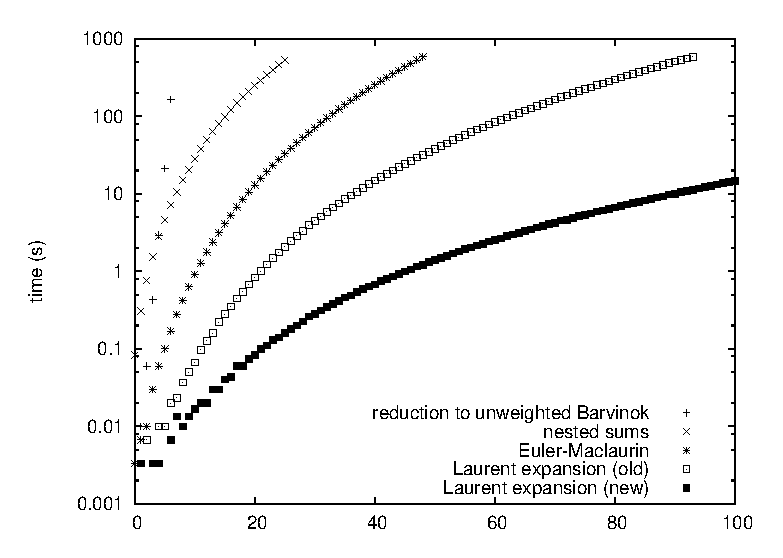
\includegraphics[width=0.9\textwidth]{sum}
\caption{Execution times for summing a monomial over a diffiuclt
non-parametric triangle}
\label{f:sum}
\end{figure}

\begin{figure}
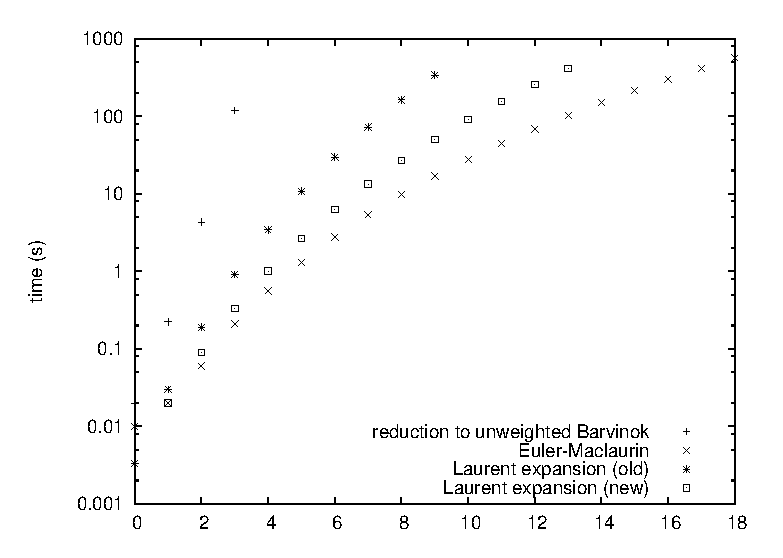
\includegraphics[width=0.9\textwidth]{sum_p}
\caption{Execution times for summing a monomial over a difficult
parametric triangle}
\label{f:sum:p}
\end{figure}

\subsection{Conversion to ``standard form''}
\label{s:standard}

Some algorithms or tools expect a polyhedron to be
specified in ``\ai{standard form}'', i.e.,
\begin{equation}
\label{eq:standard}
\begin{cases}
    \begin{aligned}
A \vec x & = \vec b \\
\vec x & \ge \vec 0
.
    \end{aligned}
\end{cases}
\end{equation}
Given an arbitrary (parametric) polyhedron
\begin{equation}
\label{eq:non-standard}
\{\,
\vec x \mid
A \vec x + \vec b(\vec p) \ge 0
\,\}
,
\end{equation}
a conversion to standard form requires the introduction
of \ai{slack variable}s and a way of dealing with variables
of \ai{unrestricted sign}.
In this section we will be satisfied with a reduction
to the form
\begin{equation}
\label{eq:standard:2}
\begin{cases}
    \begin{aligned}
A \vec x & = \vec b \\
D \vec x & \ge \vec c
,
    \end{aligned}
\end{cases}
\end{equation}
with $D$ a diagonal matrix with positive entries.
That is, we do not necessarily make all variables non-negative,
but we do ensure that they have a lower bound.
If needed, a subsequent reduction can then be performed.

The standard way of dealing with variables of unrestricted
sign is to replace a variable $x$ of unknown sign by the
difference ($x = x' - x''$) of two non-negative variables
($x', x'' \ge 0$).
However, some algorithms are somewhat sensitive with respect
to the number of variables and so we would prefer to introduce
as few extra variables as possible.
We will therefore apply a \ai{unimodular transformation}
on the variables such that all transformed variables are known
to be non-negative.

The first step is to compute the \indac{HNF} of A,
i.e., a matrix $H = A U$, with $U$ unimodular,
in column echelon form such that the
first entry in each column is positive and the other entries
on the corresponding row are non-negative and strictly smaller
than this first entry.
By reordering the rows we may assume that the top square part
of $H$ is lower-triangular.
By a further unimodular transformation, the entries
below the diagonal can be made non-positive and strictly
smaller (in absolute value) than the diagonal entry of the same row.

For each of the new variables, we can take a positive
combination of the corresponding row and the previous rows
to obtain a positive multiple of the corresponding unit vector,
implying that the variable has a lower bound.
A slack variable can then be introduced for each of the
rows in the top square part of $H'$ that is not already
a positive multiple of a unit vector and for each of
the rows below the top square part of $H'$.

\begin{example}
Consider the cone
$$
\left\{\,
\vec x \mid
\begin{bmatrix}
67 & -13 \\
-52 & 53
\end{bmatrix}
\vec x
\ge
\vec 0
\,\right\}
.
$$
This cone is already situated in the first quadrant,
but this may not be obvious from the constraints.
Furthermore, directly adding slack variables would
lead to a total of 4 variables, whereas we can also
represent this cone in standard form with only 3 variables.
We have
$$
H' =
\begin{bmatrix}
1 & 0 \\
-1331 & 2875
\end{bmatrix}
=
\begin{bmatrix}
67 & -13 \\
-52 & 53
\end{bmatrix}
\begin{bmatrix}
-6 & 13 \\
-31 & 57
\end{bmatrix}
= A U'
.
$$
Adding a slack variable for the second row of $H'$, we
obtain the equivalent problem
$$
\begin{cases}
\begin{aligned}
\begin{bmatrix}
-1331 & 2875 & -1
\end{bmatrix}
\vec x'
& =
\vec 0
\\
\vec x' & \ge \vec 0
\end{aligned}
\end{cases}
$$
with
$$
\vec x =
\begin{bmatrix}
-6 & 13 & 0 \\
-31 & 57 & 0
\end{bmatrix}
\vec x'
.
$$
\end{example}

A similar construction was used by \shortciteN[Lemma~3.10]{Eisenbrand2000PhD}
and \shortciteN{Hung1990}.

\subsection{Using TOPCOM to compute Chamber Decompositions}

In this section, we describe how to use the correspondence
between the \ai{regular triangulation}s of a point set
and the chambers of the \ai{Gale transform}
of the point set~\shortcite{Gelfand1994}
to compute the chamber decomposition of a parametric polytope.
This correspondence was also used by \shortciteN{Pfeifle2003}
\shortciteN{Eisenschmidt2007integrally}.

Let us first assume that the parametric polytope can be written as
\begin{equation}
\label{eq:TOPCOM:polytope}
\begin{cases}
    \begin{aligned}
\vec x &\ge 0
\\
A \, \vec x &\le \vec b(\vec p)
,
    \end{aligned}
\end{cases}
\end{equation}
where the right hand side $\vec b(\vec p)$ is arbitrary and
may depend on the parameters.
The first step is to add slack variables $\vec s$ to obtain
the \ai{vector partition} problem
$$
\begin{cases}
    \begin{aligned}
A \, \vec x + I \, \vec s & = \vec b(\vec p)
\\
\vec x, \vec s &\ge 0
,
    \end{aligned}
\end{cases}
$$
with $I$ the identity matrix.
Then we compute the (right) kernel $K$ of the matrix
$\begin{bmatrix}
A & I
\end{bmatrix}$, i.e.,
$$
\begin{bmatrix}
A & I
\end{bmatrix}
K
=
0
$$
and use \ai[\tt]{TOPCOM}'s \ai[\tt]{points2triangs} to
compute the \ai{regular triangulation}s of the points specified
by the rows of $K$.
Each of the resulting triangulations corresponds to a chamber
in the chamber complex of the above vector partition problem.
Each simplex in a triangulation corresponds to a parametric
vertex active on the corresponding chamber and
each point in the simplex (i.e., a row of $K$) corresponds
to a variable ($x_j$ or $s_j$) that is set to zero to obtain
this parametric vertex.
In the original formulation of the problem~\eqref{eq:TOPCOM:polytope}
each such variable set to zero reflects the saturation of the
corresponding constraint ($x_j = 0$ for $x_j = 0$ and
$\sps {\vec a_j}{\vec x} = b_j(\vec p)$ for $s_j = 0$).
A description of the chamber can then be obtained by plugging
in the parametric vertices in the remaining constraints.

\begin{example}
Consider the parametric polytope
$$
P(p,q,r) = \{\,
(i,j) \mid 0 \le i \le p \wedge
0 \le j \le 2 i + q \wedge
0 \le k \le i - p + r \wedge
p \ge 0 \wedge
q \ge 0 \wedge
r \ge 0
\,\}
.
$$
The constraints involving the variables are
$$
\begin{cases}
    \begin{aligned}
\begin{bmatrix}
1
\\
& 1
\\
& & 1
\end{bmatrix}
\begin{bmatrix}
i \\ j \\ k
\end{bmatrix}
&
\begin{matrix}
\ge
\\
\ge
\\
\ge
\end{matrix}
\begin{array}{l}
0
\\
0
\\
0
\end{array}
\\
\begin{bmatrix}
1 & 0 & 0
\\
-1 & 0 & 1
\\
-2 & 1 & 0
\end{bmatrix}
\begin{bmatrix}
i \\ j \\ k
\end{bmatrix}
&
\begin{matrix}
\le
\\
\le
\\
\le
\end{matrix}
\begin{array}{l}
p
\\
q
\\
-p + r
\end{array}
    \end{aligned}
\end{cases}
$$
We have
$$
\begin{bmatrix}
   1 &   0  &  0 &   1  &  0  &  0  \\
  -1 &   0  &  1 &   0  &  1  &  0  \\
  -2 &   1  &  0 &   0  &  0  &  1  \\
\end{bmatrix}
\begin{bmatrix}
  -1  &  0 &   0  \\
  -2  &  0 &  -1  \\
  -1  & -1 &   0  \\
   1  &  0 &   0  \\
   0  &  1 &   0  \\
   0  &  0 &   1  \\
\end{bmatrix}
= 0
$$

Computing the \ai{regular triangulation}s of the rows of $K$
using \ai[\tt]{TOPCOM}, we obtain
\begin{verbatim}
> cat e2.topcom
[
[  -1    0    0 ]
[  -2    0   -1 ]
[  -1   -1    0 ]
[   1    0    0 ]
[   0    1    0 ]
[   0    0    1 ]
]
> points2triangs --regular < e2.topcom 
T[1]:={{0,1,2},{1,2,3},{0,1,4},{1,3,4},{0,2,5},{2,3,5},{0,4,5},{3,4,5}};
T[2]:={{1,2,3},{1,3,4},{2,3,5},{3,4,5},{1,2,5},{1,4,5}};
T[3]:={{1,2,3},{1,3,4},{2,3,5},{3,4,5},{1,2,4},{2,4,5}};
\end{verbatim}

We see that we have three chambers in the decomposition,
one with 8 vertices and two with 6 vertices.
Take the second vertex (``\verb+{1,2,3}+'') of the first chamber.
This vertex corresponds
to the saturation of the constraints $j \ge 0$, $k \ge 0$
and $i \le p$, i.e., $(i,j,k) = (p,0,0)$.  Plugging in this
vertex in the remaining constraints, we see that it is only valid
in case $p \ge 0$, $r \ge 0$ and $2p + q \ge 0$.
For the remaining vertices of the first chamber, we similarly find
\\
\begin{tabular}{ccc}
% e0
\verb+{0,1,2}+ & $(0,0,0)$ & $p \ge 0$, $-q + r \ge 0$ and $q \ge 0$
\\
% 70
\verb+{1,2,3}+ & $(p,0,0)$ & $p \ge 0$, $r \ge 0$ and $2p + q \ge 0$
\\
% c8
\verb+{0,1,4}+ & $(0,0,-p+r)$ & $-q + r \ge 0$, $p \ge 0$ and $q \ge 0$
\\
% 58
\verb+{1,3,4}+ & $(p,0,r)$ & $p \ge 0$, $r \ge 0$ and $2p + q \ge 0$
\\
% a4
\verb+{0,2,5}+ & $(0,q,0)$ & $q \ge 0$, $p \ge 0$ and $-q + r \ge 0$
\\
% 34
\verb+{2,3,5}+ & $(p, 2p+q, 0)$ & $p \ge 0$, $2p + q \ge 0$ and $r \ge 0$
\\
% 8c
\verb+{0,4,5}+ & $(0, q, -p+r)$ & $q \ge 0$, $-q + r \ge 0$ and $p \ge 0$
\\
% 1c
\verb+{3,4,5}+ & $(p, 2p+q, r)$ & $p \ge 0$, $2p + q \ge 0$ and $r \ge 0$
\end{tabular}
\\
Combining these constraints with the initial constraints of the problem
on the parameters
$p \ge 0$, $q \ge 0$ and $r \ge 0$, we find the chamber
$
\{\,
(p,q,r) \mid p \ge 0 \wedge -p + r \ge 0 \wedge q \ge 0
\,\}
$.
For the second chamber, we have
\\
\begin{tabular}{ccc}
% 70
\verb+{1,2,3}+ & $(p,0,0)$ & $p \ge 0$, $r \ge 0$ and $2p + q \ge 0$
\\
% 58
\verb+{1,3,4}+ & $(p,0,r)$ & $p \ge 0$, $r \ge 0$ and $2p + q \ge 0$
\\
% 34
\verb+{2,3,5}+ & $(p, 2p+q, 0)$ & $p \ge 0$, $2p + q \ge 0$ and $r \ge 0$
\\
% 1c
\verb+{3,4,5}+ & $(p, 2p+q, r)$ & $p \ge 0$, $2p + q \ge 0$ and $r \ge 0$
\\
% 64
\verb+{1,2,5}+ & $(-\frac q 2,0,0)$ &
	$-q \ge 0$, $2p + q \ge 0$ and $-2p -q+2r \ge 0$
\\
% 4c
\verb+{1,4,5}+ & $(-\frac q 2,0,-p-\frac q 2+r)$ &
	$-q \ge 0$, $-2p -q+2r \ge 0$ and $2p + q \ge 0$
\end{tabular}
\\
The chamber is therefore
$
\{\,
(p,q,r) \mid q = 0 \wedge p \ge 0 \wedge -p +r \ge 0
\,\}
$.
Note that by intersecting with the initial constraints this chamber
is no longer full-dimensional and can therefore be discarded.
Finally, for the third chamber, we have
\\
\begin{tabular}{ccc}
% 70
\verb+{1,2,3}+ & $(p,0,0)$ & $p \ge 0$, $r \ge 0$ and $2p + q \ge 0$
\\
% 58
\verb+{1,3,4}+ & $(p,0,r)$ & $p \ge 0$, $r \ge 0$ and $2p + q \ge 0$
\\
% 34
\verb+{2,3,5}+ & $(p, 2p+q, 0)$ & $p \ge 0$, $2p + q \ge 0$ and $r \ge 0$
\\
% 1c
\verb+{3,4,5}+ & $(p, 2p+q, r)$ & $p \ge 0$, $2p + q \ge 0$ and $r \ge 0$
\\
% 68
\verb+{1,2,4}+ & $(p-r,0,0)$ &
	$p -r \ge 0$, $r \ge 0$ and $2p +q -2r \ge 0$
\\
% 2c
\verb+{2,4,5}+ & $(p-r,2p+q-2r, 0)$ &
	$p -r \ge 0$, $2p +q -2r \ge 0$ and $r \ge 0$
\end{tabular}
\\
The chamber is therefore
$
\{\,
(p,q,r) \mid p - r \ge 0 \wedge q \ge 0 \wedge r \ge 0
\,\}
$.
\end{example}

Now let us consider general parametric polytopes.
First note that we can follow the same procedure as above
if we replace $\vec x$ by $\vec x' - \vec c(\vec p)$
in \eqref{eq:TOPCOM:polytope}, i.e.,
if our problem has the form
\begin{equation}
\label{eq:TOPCOM:polytope:2}
\begin{cases}
    \begin{aligned}
\vec x' &\ge \vec c(\vec p)
\\
A \, \vec x' &\le \vec b(\vec p) + A \vec c(\vec p)
,
    \end{aligned}
\end{cases}
\end{equation}
as saturating a constraint $x_i = 0$ is equivalent
to saturating the constraint $x_i' = c_i(\vec p)$
and, similarly, $\sps {\vec a_j}{\vec x} = b_j(\vec p)$
is equivalent to
$\sps {\vec a_j}{\vec x'} = b_j(\vec p) + \sps {\vec a_j}{\vec c(\vec p)}$.

In the general case, the problem has the form
$$
A \vec x \ge \vec b(\vec p)
$$
and then we apply the technique of \autoref{s:standard}.
Let $A'$ be a non-singular square submatrix of $A$ with the same number
of columns and compute the (left) \indac{HNF} $H = A' U$ with $U$ unimodular
and $H$ lower-triangular with non-positive elements below the diagonal.
Replacing $\vec x$ by $U \vec x'$, we obtain
$$
\begin{cases}
    \begin{aligned}
H \vec x' &\ge \vec b'(\vec p)
\\
-A''U \, \vec x' &\le -\vec b''(\vec p)
,
    \end{aligned}
\end{cases}
$$
with $A''$ the remaining rows of $A$ and $\vec b(\vec p)$ split
in the same way.
If $H$ happens to be the identity matrix, then our problem is
of the form \eqref{eq:TOPCOM:polytope:2} and we already know how
to solve this problem.
Note that, again, saturating any of the transformed constraints
in $\vec x'$ is equivalent to saturating the corresponding constraint
in $\vec x$.  We therefore only need to compute $-A'' U$ for the
computation of the kernel $K$.  To construct the parametric vertices
in the original coordinate system, we can simply use the original
constraints.
The same reasoning holds if $H$ is any diagonal matrix, since
we can virtually replace $H \vec x$ by $\vec x'$ without affecting
the non-negativity of the variables.

If $H$ is not diagonal, then we can introduce new constraints
$x'_j \ge d(\vec p)$, where $d(\vec p)$ is some symbolic constant.
These constraints do not remove any solutions
since each row in $H$ expresses that the corresponding variable is
greater than or equal to a non-negative combination of the
previous variables plus some constant.
We can then proceed as before.  However, to reduce unnecessary computations
we may remove from $K$ the rows that correspond to these new rows.
Any solution saturating the new constraint, would also saturate
the corresponding constraint $\vec h_j^\T$ and all
the constraints corresponding to the non-zero
entries in $\vec h_j^\T$.
If a chamber contains a vertex obtained by saturating such a new
constraint, it would appear multiple times in the same chamber,
each time combined with different constraints from the above set.
Furthermore, there would also be another (as it turns out, identical)
chamber where the vertex is only defined by the other constraints.

\begin{example}
Consider the parametric polytope
$$
P(n) = \{\,
(i,j) \mid
1 \le i \wedge 2 i \le 3 j \wedge j \le n
\,\}
.
$$
The constraints are
$$
\begin{bmatrix}
1 & 0 \\
-2 & 3 \\
0 & -1
\end{bmatrix}
\begin{bmatrix}
i \\ j
\end{bmatrix}
\ge
\begin{bmatrix}
1 \\
0 \\
-n
\end{bmatrix}
.
$$
The top $2 \times 2$ submatrix is already in \indac{HNF}.
We have $3 j \ge 2i \ge 2$, so we can add a constraint
of the form $j \ge c(n)$ and obtain
$$
\begin{bmatrix}
A & I
\end{bmatrix}
=
\begin{bmatrix}
0 & 1 & 1 & 0
\\
2 & -3 & 0 & 1
\end{bmatrix}
,
$$
while $K$ with $\begin{bmatrix}A & I\end{bmatrix} K = 0$ is given
by
$$
\begin{bmatrix}
0 & 1 & 1 & 0
\\
2 & -3 & 0 & 1
\end{bmatrix}
\begin{bmatrix}
1 & 0 \\
0 & 1 \\
0 & -1 \\
-2 & 3
\end{bmatrix}
.
$$
The second row of $K$ corresponds to the second variable,
which in turn corresponds to the newly added constraint.
Passing all rows of $K$ to \ai[\tt]{TOPCOM} we would get
\begin{verbatim}
> points2triangs --regular <<EOF
> [[1 0],[0,1],[0,-1],[-2,3]]
> EOF
T[1]:={{0,1},{0,2},{1,3},{2,3}};
T[2]:={{0,2},{2,3},{0,3}};
T[3]:={};
\end{verbatim}
The first vertex in the first chamber saturates the second row
(row 1) and therefore saturates both the first (0) and fourth (3)
and it appears a second time as \verb+{1,3}+.  Combining
these ``two'' vertices into one as \verb+{0,3}+ results in the
second (identical) chamber.
Removing the row corresponding to the new constraint from $K$
we remove the duplicates
\begin{verbatim}
> points2triangs --regular <<EOF
> [[1 0],[0,-1],[-2,3]]
> EOF
T[1]:={{0,1},{1,2},{0,2}};
T[2]:={};
\end{verbatim}
Note that in this example, we also could have interchanged
the second and the third constraint and then have replaced $j$ by $-j'$.
\end{example}

In practice, this method of computing a \ai{chamber decomposition}
does not seem to perform very well, mostly because
\ai[\tt]{TOPCOM} can not exploit all available information
about the parametric polytopes and will therefore compute
many redundant triangulations/chambers.
In particular, any chamber that does not intersect with
the parameter domain of the parametric polytope, or only
intersects in a face of this parameter domain, is completely redundant.
Furthermore, if the parametric polytope is not simple, then many
different combinations of the constraints will lead to the same parametric
vertex.  Many triangulations will therefore correspond to one and the
same chamber in the chamber complex of the parametric polytope.
For example, for a dilated octahedron, \ai[\tt]{TOPCOM} will
compute 150 triangulations/chambers, 104 of which are empty,
while the remaining 46 refer to the same single chamber.


\subsection{Computing the Hilbert basis of a cone}
\label{s:hilbert}

To compute the \ai{Hilbert basis} of a cone, we use
the \ai[\tt]{zsolve} library from \ai[\tt]{4ti2} \shortcite{4ti2},
which implements the technique of \shortciteN{Hemmecke2002Hilbert}.
We first remove all equalities from the cone through unimodular
transformations and then apply the technique of \autoref{s:standard}
to put the cone in ``standard form''.  Note that for a (non-parametric)
cone the constant term $\vec b$ in \eqref{eq:non-standard} is $\vec 0$.
The constraints $D \vec x \ge \vec c = \vec 0$ of \eqref{eq:standard:2}
are therefore equivalent to $\vec x \ge \vec 0$.


\subsection{Integer Feasibility}
\label{s:feasibility}

For testing whether a polytope $P \subset \QQ^d$ contains any integer points,
we use the technique of~\shortciteN{Cook1993implementation},
based on \ai{generalized basis reduction}.

The technique basically looks for a ``short vector'' $\vec c$ in the
lattice $\ZZ^d$, where shortness is measured in terms of
the \ai{width} of the polytope $P$ along that direction,
\begin{align*}
\width_{\vec c} P
& =
\max \{\, \sp c x \mid \vec x \in P \,\}
-
\min \{\, \sp c x \mid \vec x \in P \,\}
\\
& =
\max \{\, \sps {\vec c} {\vec x - \vec y} \mid \vec x, \vec y \in P \,\}
.
\end{align*}
The \defindex{lattice width} is the minimum width over all
non-zero integer directions:
$$
\width P =
\min_{\vec c \in \ZZ^d \setminus \{ \vec 0 \} } \width_{\vec c} P
.
$$
If the dimension $d$ is fixed then
the lattice width of any polytope $P \subset \QQ^d$
containing no integer points is bounded by a constant%
~\shortcite{Lagarias90,Barvinok02,Banaszczyk1999flatness}.
If we slice the polytope using hyperplanes orthogonal
to a short direction, i.e., a direction where the width
is small, we will therefore only need to inspect
``few'' of them before either finding one with an integer point,
or running out of hyperplanes, meaning that the
polytope did not contain any integer points.
Each slice is checked for integer points by applying
the above method recursively.

A nice feature of this technique is that it will
not only tell you if there is any integer point
in the given polytope, but it will actually compute
one if there is any.

The short vector is obtained as the first vector
of a ``reduced basis'' of the lattice $\ZZ^d$ with respect
to the polytope.
In particular, the first vector $\vec b_1$ of this reduced basis
will satisfy
$$
\width_{\vec b_1} P
\le
\frac{\width P}
{\left(\frac 1 2 - \varepsilon\right)^{d-1}}
,
$$
with $0 < \varepsilon < 1/2$ a fixed constant.
That is, the width in direction $\vec b_1$ is no more than a constant
factor bigger than the lattice width.
See~\shortcite{Cook1993implementation} for details.
In our implementation we use $\varepsilon = 1/4$.
When used in the above integer feasibility testing algorithm,
we will also terminate the reduced basis computation
as soon as the width along the first basis vector is smaller than 2.
This means that there will be at most 2 slices orthogonal to the chosen
direction.

The computation of the above reduced basis requires the solution
of many linear programs, for which we use any of the following
external solvers:
\begin{itemize}
\item \ai[\tt]{GLPK}~\shortcite{GLPK}

This solver is based on double precision floating point arithmetic and
may therefore not be suitable if the coefficients of the constraints
describing the polytope are large.

\item \ai[\tt]{cdd}~\shortcite{cdd}

This solver is based on exact integer arithmetic.
Note that you need version \verb+cddlib 0.94e+ or newer.
Earlier versions (\verb+0.93+--\verb+0.94d+) have
a bug that may sometimes result in a polytope being
reported as (rationally) empty even though it is not.

\item \piplib/~\shortcite{Feautrier:PIP}

This solver is also based on exact integer arithmetic
and uses the \ai{dual simplex} method to solve a linear program.
Two versions are available, \ai[\tt]{pip} will present the
original program to \piplib/, while \ai[\tt]{pip-dual} will present
the dual program to \piplib/, effectively having it apply the primal
simplex method to the original problem.
The latter may seem more appropriate since the computation
of the reduced basis only requires the dual solution of
any linear program.  However, in practice, it appears
that \ai[\tt]{pip} is often faster than \ai[\tt]{pip-dual}.
\end{itemize}
The LP solver to use can be selected with the \ai[\tt]{--gbr} option.


\subsection{Computing the integer hull of a polyhedron}
\label{s:integer:hull}

For computing the \ai{integer hull} of a polyhedron,
we first describe how to compute the convex hull of a set
given as an oracle for optimizing a linear objective
function over the set and then
we explain how to optimize a linear objective function over
the integer points of a polyhedron.
Applying the first with the second as \ai{optimization oracle}
yields a method for computing the requested integer hull.

\subsubsection{Computing the convex hull based on an optimization oracle}

The algorithm described below is presented by
\shortciteN[Remark~2.5]{Cook1992} as an extension of the
algorithm by \shortciteN[Section~3]{Edmonds82} for computing
the {\em dimension} of a polytope for which only an optimization oracle
is available.  The algorithm is described in a bit more detail
by \shortciteN{Eisenbrand2000PhD} and reportedly stems from
\shortciteN{Hartmann1989PhD}.
Essentially the same algorithm has also been implemented
by \shortciteN{Huggins06}, citing
\ai{beneath/beyond}~\shortcite{Preparata1985} as his inspiration.

The algorithm start out from an initial set of points from
the set $S$.  After computing the convex hull of this set
of points, we take one of its bounding constraints and use
the optimization oracle
to compute an optimal point in $S$ (but on the other side
of the bounding hyperplane) along the
outer normal of this bounding constraint.
If a new point is found, it is added to the set of points
and a new convex hull is computed, or the old one is adapted
in a beneath/beyond fashion.  Otherwise, the chosen bounding constraint
is also a bounding constraint of $S$ and need not be considered anymore.
The process continues until all bounding constraints in the
description of the current convex hull have been considered.

In principle, the initial set of points in the above algorithm
may be empty, with a ``convex hull'' described by a set of
conflicting constraints and each equality in the description of any
intermediate lower-dimensional convex hull being considered
as a pair of bounding constraints with opposite outer normals.
However, in our implementation, we have chosen to first compute
a maximal set of affinely independent points by first taking any
point from $S$ and then adding points from $S$ not on one of
the equalities satisfied by all points found so far.
This allows us to not have to worry about equalities in the
main algorithm.
In the case of the computation of the integer hull, finding
these affinely independent points can be accomplished using the technique of
\autoref{s:feasibility}.

\begin{figure}
\intercol=0.58cm
\begin{xy}
<\intercol,0pt>:<0pt,\intercol>::
\POS(-1,0)*\xybox{
\def\latticebody{\POS="c"+(0,0.5)\ar@{--}"c"+(0,6.5)}%
\POS0,{\xylattice{1}{6}00}%
\def\latticebody{\POS="c"+(0.5,0)\ar@{--}"c"+(6.5,0)}%
\POS0,{\xylattice00{1}6}%
\POS@i@={(1.5,2.75),(5.75,2.25),(5.5,5.25),(2.75,4.75),(1.5,2.75)},
{0*\xypolyline{}}
\POS@i@={(2,3),(3,3),(3,4),(2,3)},{0*[|(3)]\xypolyline{}}
\POS(2,3)*{\bullet}
\POS(3,3)*{\bullet}
\POS(3,4)*{\bullet}
\POS(3,3.5)\ar(3.5,3.5)
\POS(5,3)*{\circ}
\POS(5,4)*{\circ}
\POS(5,5)*{\circ}
}
\POS(6,0)*\xybox{
\def\latticebody{\POS="c"+(0,0.5)\ar@{--}"c"+(0,6.5)}%
\POS0,{\xylattice{1}{6}00}%
\def\latticebody{\POS="c"+(0.5,0)\ar@{--}"c"+(6.5,0)}%
\POS0,{\xylattice00{1}6}%
\POS@i@={(1.5,2.75),(5.75,2.25),(5.5,5.25),(2.75,4.75),(1.5,2.75)},
{0*\xypolyline{}}
\POS@i@={(2,3),(5,3),(3,4),(2,3)},{0*[|(3)]\xypolyline{}}
\POS(2,3)*{\bullet}
\POS(5,3)*{\bullet}
\POS(3,4)*{\bullet}
\POS(4,3.5)\ar(4.25,4)
\POS(5,5)*{\circ}
}
\POS(13,0)*\xybox{
\def\latticebody{\POS="c"+(0,0.5)\ar@{--}"c"+(0,6.5)}%
\POS0,{\xylattice{1}{6}00}%
\def\latticebody{\POS="c"+(0.5,0)\ar@{--}"c"+(6.5,0)}%
\POS0,{\xylattice00{1}6}%
\POS@i@={(1.5,2.75),(5.75,2.25),(5.5,5.25),(2.75,4.75),(1.5,2.75)},
{0*\xypolyline{}}
\POS@i@={(2,3),(5,3),(5,5),(3,4),(2,3)},{0*[|(3)]\xypolyline{}}
\POS(2,3)*{\bullet}
\POS(5,3)*{\bullet}
\POS(5,5)*{\bullet}
\POS(3,4)*{\bullet}
}
\end{xy}
\caption{The integer hull of a polytope}
\label{f:integer:hull}
\end{figure}

\begin{example}
Assume we want to compute the integer hull of the polytope in the left part
of \autoref{f:integer:hull}.
We first compute a set of three affinely independent points,
shown in the same part of the figure.
Of the three facets of the corresponding convex hull,
optimization along the outer normal (depicted by an arrow in the figure)
of only one facet will yield any additional points.  The other two
are therefore facets of the integer hull.
Optimization along the above outer normal may yield any of the
points marked by a $\circ$.
Assuming it is the bottom one, we end up with the updated
convex hull in the middle of the figure.  This convex hull
has only one new facet.  Adding the point found by optimizing
over this facet's outer normal, we obtain the convex hull
on the right of the figure.
There are two new facets, but neither of them yields any
further points.  We have therefore found the integer hull
of the polytope.
\end{example}

\subsubsection{Optimization over the integer points of a polyhedron}
\label{s:optimization}

We assume that we want to find the {\em minimum} of
some linear objective function.  When used in the computation
of the integer hull of some polytope, the objective function
will therefore correspond to the inner normal of some facet.

During our search for an optimal integer point with respect
to some objective function, we will keep track of the best
point so far as well as a lower bound $l$
and an upper bound $u$ such that the value at the optimal point
(if it is better than the current best) lies between those
two bounds.
Initially, there is no best point yet and values for $l$ and $u$
may be obtained from optimization over the linear relaxation.
When used in the computation of the integer hull of some polytope,
the upper bound $u$ is one less than the value attained on
the given facet of the current approximation.

As long as $l \le u$, we perform the following steps
\begin{itemize}
\item use the integer feasibility technique of \autoref{s:feasibility}
to test whether there is any integer point with value in
$[l,u']$, where $u'$ is
\begin{itemize}
\item $u$ if the previous test for an integer point did not produce a point
\item $l+\floor{\frac{u-l-1}2}$
 if the previous test for an integer point {\em did\/} produce a point
\end{itemize}
\item if a point is found, then remember it as the current best
and replace $u$ by the value at this point minus one,
\item otherwise, replace $l$ by $u'+1$.
\end{itemize}
When used in the computation of the integer hull of some polytope,
it is useful to not only keep track of the best point so far,
but of all points found.
These points will all lie outside of the current approximation
of the integer hull and adding them all instead of just one,
will typically get us to the complete integer hull quicker.

\begin{figure}
\intercol=0.7cm
\begin{xy}
<\intercol,0pt>:<0pt,\intercol>::
\POS(0.5,0)\ar@{-}(16.5,0)
\def\latticebody{\POS="c"+(0,-0.2)\ar@{--}"c"+(0,0.2)\POS"c"*++!D{\the\latticeA}}%
\POS0,{\xylattice{1}{16}00}%
\POS(6,0)*!C{\bullet}
\POS(7,0)*{\bullet}
\POS(8,0)*{\bullet}
\POS(12,0)*{\bullet}
\POS(13,0)*{\bullet}
\POS(14,0)*{\bullet}
\POS(15,0)*{\bullet}
\POS(16,0)*{\bullet}
\POS(1,-1)\ar@{-}(16,-1)
\POS(8,-1)*{\bullet}
\POS(1,-2)\ar@{-}(4,-2)
\POS(5,-3)\ar@{-}(7,-3)
\POS(6,-3)*{\bullet}
\POS(4.9,-4)\ar@{-}(5.1,-4)
\end{xy}
\caption{The integer points of a polytope projected on an objective function}
\label{f:hull:projected}
\end{figure}

\begin{example}
\label{ex:hull:projected}
Assume that the values of some objective function attained
by the integer points of some polytope are as shown in
\autoref{f:hull:projected} and assume we know that the optimal
value lies between 1 and 16.
In the first step we would look for a point attaining a value
in the interval $[1,16]$.  Suppose this yields a point attaining
the value $8$ (second line of the figure).  We record this point
as the current best and update the search interval to $[1,7]$.
In the second step, we look for a point attaining a value
in the interval $[1,4]$, but find nothing and set the search interval
to $[5,7]$.
In the third step, we consider the interval $[5,7]$ and find
a point attaining the value 6.  We update the current best value
and set the search interval to $[5,5]$.
In the fourth step, we consider the interval $[5,5]$, find no
points and update the interval to ``$[6,5]$''.
Since the lower bound is now larger than the upper bound, the
algorithm terminates, returning the best or all point(s) found.
\end{example}


\subsection{Computing the integer hull of a truncated cone}
\label{s:hull:cone}

In \autoref{s:width} we will need to compute the \ai{integer hull}
of a cone with the origin removed ($C \setminus \{ \vec 0 \}$).

\subsubsection{Using the Hilbert basis of the cone}

As proposed by \shortciteN{Koeppe2007personal},
one way of computing this integer hull is to first compute
the \ai{Hilbert basis} of $C$ (see \autoref{s:hilbert})
and to then remove from that Hilbert basis the points that
are not vertices of the integer hull of $C \setminus \{ \vec 0 \}$.
The Hilbert basis of $C$ is the minimal set of points
$\vec b_i \in C \cap \ZZ^d$ such that every integer point
$\vec x \in C \cap \ZZ^d$ can be written as a non-negative
{\em integer} combination of the $\vec b_i$.
The vertices $\vec v_j$ of the integer hull of $C \setminus \{ \vec 0 \}$
are such that every integer point
$\vec x \in (C \cap \ZZ^d) \setminus \{ \vec 0 \}$ can
be written as s non-negative {\em rational} combination of $\vec v_j$.
Clearly, any $\vec v_j$ is also a $\vec b_i$ since $\vec v_j$ can
not be written as the sum of a (rational) convex combination of
other integer points in $(C \cap \ZZ^d) \setminus \{ \vec 0 \}$
and a non-negative combination of the extremal rays $\vec r_k$ of $C$.
A fortiori, it can therefore not be written as an integer combination
of other integer points in $C$.
To obtain the $\vec v_j$ from the $\vec b_i$ we therefore simply
need to remove first $(0,0)$ and then those $\vec b_i$ that are
not an extremal ray and that {\em can} be written as a combination
$$
\vec b_i = \sum_{j \ne i} \vec \alpha_j \vec b_j + \sum_k \beta_k \vec r_k
\qquad\text{with $\alpha_j, \beta_k \ge 0$ and $\sum_{j \ne i} \alpha_j = 1$}
.
$$
Since the $\vec r_k$ are also among the $\vec b_j$, this can
be simplified to checking whether there exists a rational
solution for $\vec \alpha_j$ to
$$
\vec b_i = \sum_{j \ne i} \vec \alpha_j \vec b_j
\qquad\text{with $\alpha_j \ge 0$ and $\sum_{j \ne i} \alpha_j \ge 1$}
.
$$

\begin{figure}
\intercol=1.1cm
\begin{xy}
<\intercol,0pt>:<0pt,\intercol>::
\POS@i@={(3,-4.5),(2,-3),(1,-1),(1,1),(3,4),(4.125,5.5),(5.5,5.5),(5.5,-4.5)},{0*[grey]\xypolyline{*}}
\def\latticebody{\POS="c"+(0,-4.5)\ar@{--}"c"+(0,5.5)}%
\POS0,{\xylattice{-0}{5}00}%
\def\latticebody{\POS="c"+(-0.5,0)\ar@{--}"c"+(5.5,0)}%
\POS0,{\xylattice00{-4}5}%
\POS0\ar(2,-3)
\POS0\ar(3,4)
\POS(2,-3)*{\bullet}
\POS(3,4)*{\bullet}
\POS(1,1)*{\bullet}
\POS(1,-1)*{\bullet}
\POS(1,0)*{\bullet}
\POS(2,-3)*{\times}
\POS(3,4)*{\times}
\POS(1,1)*{\times}
\POS(1,-1)*{\times}
\end{xy}
\caption{The Hilbert basis and the integer hull of a truncated cone}
\label{f:hilbert:hull}
\end{figure}

\begin{example} \label{ex:hilbert:hull}
Consider the cone
$$
C = \poshull \,\{(2,-3), (3,4)\}
,
$$
shown in Figure~\ref{f:hilbert:hull}.
The Hilbert basis of this cone is
$$\{(0,0),(2,-3),(3,4),(1,1),(1,-1),(1,0)\}.$$
We have $(1,0) = \frac 1 2 (1,1) + \frac 1 2 (1,-1)$,
while $(1,1)$ and $(1,-1)$ can not be written as
overconvex combinations of the other $\vec b_i \ne \vec 0$.
The vertices of the integer hull of $C \setminus \{ \vec 0 \}$
are therefore
$$\{(2,-3),(3,4),(1,1),(1,-1)\}.$$
\end{example}

\subsubsection{Using generalized basis reduction}
\label{s:hull:cone:gbr}

Another way of computing the integer hull of a truncated cone is to apply
the method of \autoref{s:integer:hull}.
In this case, the initial set of points will consist
of (the smallest integer representatives of) the extremal rays
of the cone, together with the extremal rays themselves.
That is, if $C = \poshull \, \{ \vec r_j \}$ with
$\vec r_j \in \ZZ^d$, then our initial approximation of the
integer hull of $C \setminus \{ \vec 0 \}$ is
$$
\convhull \, \{ \vec r_j \} + \poshull \, \{ \vec r_j \}
.
$$
Furthermore, we need never consider any
of the bounding constraints that are also bounding constraints
of the original cone.
When optimizing along the normal of any of the other facets, we can
take the lower bound to be $1$.  This will ensure that
the origin is excluded, without excluding any other integer points.

\begin{figure}
\intercol=0.5cm
\begin{xy}
<\intercol,0pt>:<0pt,\intercol>::
\POS(0,0)*\xybox{
\POS@i@={(3,-4.5),(2,-3),(3,4),(4.125,5.5),(5.5,5.5),(5.5,-4.5)},{0*[grey]\xypolyline{*}}
\def\latticebody{\POS="c"+(0,-4.5)\ar@{--}"c"+(0,5.5)}%
\POS0,{\xylattice{-0}{5}00}%
\def\latticebody{\POS="c"+(-0.5,0)\ar@{--}"c"+(5.5,0)}%
\POS0,{\xylattice00{-4}5}%
\POS0\ar(2,-3)
\POS0\ar(3,4)
\POS(2,-3)*{\bullet}
\POS(3,4)*{\bullet}
\POS(1,1)*{\circ}
}
\POS(8,0)*\xybox{
\POS@i@={(3,-4.5),(2,-3),(1,1),(3,4),(4.125,5.5),(5.5,5.5),(5.5,-4.5)},{0*[grey]\xypolyline{*}}
\def\latticebody{\POS="c"+(0,-4.5)\ar@{--}"c"+(0,5.5)}%
\POS0,{\xylattice{-0}{5}00}%
\def\latticebody{\POS="c"+(-0.5,0)\ar@{--}"c"+(5.5,0)}%
\POS0,{\xylattice00{-4}5}%
\POS0\ar(2,-3)
\POS0\ar(3,4)
\POS(2,-3)*{\bullet}
\POS(3,4)*{\bullet}
\POS(1,1)*{\bullet}
\POS(1,-1)*{\circ}
}
\POS(16,0)*\xybox{
\POS@i@={(3,-4.5),(2,-3),(1,-1),(1,1),(3,4),(4.125,5.5),(5.5,5.5),(5.5,-4.5)},{0*[grey]\xypolyline{*}}
\def\latticebody{\POS="c"+(0,-4.5)\ar@{--}"c"+(0,5.5)}%
\POS0,{\xylattice{-0}{5}00}%
\def\latticebody{\POS="c"+(-0.5,0)\ar@{--}"c"+(5.5,0)}%
\POS0,{\xylattice00{-4}5}%
\POS0\ar(2,-3)
\POS0\ar(3,4)
\POS(2,-3)*{\bullet}
\POS(3,4)*{\bullet}
\POS(1,1)*{\bullet}
\POS(1,-1)*{\bullet}
}
\end{xy}
\caption{The integer hull of a truncated cone}
\label{f:cone:integer:hull}
\end{figure}

\begin{example}
Consider once more the cone
$$
C = \poshull \,\{(2,-3), (3,4)\}
$$
from Example~\ref{ex:hilbert:hull}.
The initial approximation is
$$
C = \convhull \,\{(2,-3), (3,4)\} + \poshull \,\{(2,-3), (3,4)\}
,
$$
which is shown on the left of \autoref{f:cone:integer:hull}.
The only bounding constraint that does not correspond to a
bounding constraint of $C$ is $7 x - y \ge 17$.
In the first step, we will therefore look for a point
minimizing $7 x - y$ with values in the interval $[1,16]$.
All values of this objective function in the given interval
attained by points in $C$ are shown in \autoref{f:hull:projected}.
From Example~\ref{ex:hull:projected}, we know that the optimal
value is $6$ and this corresponds to the point $(1,1)$.
Adding this point to our hull, we obtain the approximation
in the middle of \autoref{f:cone:integer:hull}.
This approximation has two new facets.
The bounding constraint $3x - 2 y \ge 1$ will not produce
any new points since we would be looking for one in the
interval ``$[1,0]$''.
The other new bounding constraint is $4x + y \ge 5$.
Minimizing $4 x+ y$ with values in the interval $[1,4]$,
we find the minimal value $3$ corresponding to the point $(1,-1)$.
Adding this point, we obtain the complete integer hull
shown on the right of \autoref{f:cone:integer:hull}.
Note that if in the first step we would have added not only
the point corresponding to the optimal value, but instead
all points found in Example~\ref{ex:hull:projected},
then we would have obtained the complete integer hull directly.
\end{example}


\subsection{Computing the lattice width of a parametric polytope}
\label{s:width}

To compute the \ai{lattice width} of a \ai{parametric polytope},
we essentially use the technique of \shortciteN{Eisenbrand2007parameterised},
which improves upon the technique of \shortciteN{Kannan1992}.
Given a parametric polytope
$$
P(\vec p) = \{\, \vec x \mid A \vec x + \vec b(\vec p) \ge \vec 0 \,\}
,
$$
the width along a direction $\vec c$ is defined in the same
way as for non-parametric polytopes (see \autoref{s:feasibility}),
\begin{equation}
\label{eq:width}
\width_{\vec c} P(\vec p)
=
\max \{\, \sp c x \mid \vec x \in P(\vec p) \,\}
-
\min \{\, \sp c x \mid \vec x \in P(\vec p) \,\}
.
\end{equation}
The \defindex{lattice width} is the minimum width over all
non-zero integer directions:
$$
\width P(\vec p) =
\min_{\vec c \in \ZZ^d \setminus \{ \vec 0 \} } \width_{\vec c} P(\vec p)
.
$$
We assume that the parameter domain $Q$ of $P(\vec p)$, i.e., the
set of parameter values for which $P(\vec p) \ne \emptyset$,
is full-dimensional and that for each $\vec p$ from the interior
of $Q$, $P(\vec p)$ is also full-dimensional.

Clearly, for any given direction $\vec c$, the minimum and
maximum in \eqref{eq:width} are attained at (different)
vertices of $P(\vec p)$.
The idea of the algorithm is then to consider all pairs
of parametric vertices of $P(\vec p)$, to compute all candidate
integer directions for a given pair of vertices and then to
compute the minimum width over all candidate integer directions
found.

For any given parametric vertex $\vec v(\vec p)$, the (rational)
directions for which this vertex is minimal can be found as follows.
Let $\vec v(\vec p) + C$ be the \ai{vertex cone} of $\vec v(\vec p)$.
If $\vec v(\vec p)$ is minimal for $\vec c$, then all other points
in the vertex cone must yield a bigger or equal value, i.e.,
$\sp y c \ge 0$ for all $\vec y \in C$.
The set of directions is therefore the \ai{polar cone} $C^*$ of $C$.
Note that, in principle, we should only do this for pairs
of vertices that have a common activity domain, where the
activity domains have been partially opened using the
technique of \autoref{p:inclusion-exclusion} to avoid
multiple vertices that coincide on a lower-dimensional
chamber to all be considered on this intersection.
However, this optimization has currently not been implemented.

Given a pair of vertices $\vec v_1(\vec p)$ and $\vec v_2(\vec p)$,
we may assume that $\vec v_1(\vec p)$ attains the minimum and
$\vec v_2(\vec p)$ attains the maximum.
If $\vec v_1(\vec p) + C_1$ and $\vec v_2(\vec p) + C_2$ are the
corresponding vertex cones, then the set of (rational) directions for this
pair of vertices is
$$
C_{1,2} = \left( C_1^* \cap -C_2^* \right) \setminus \{ \vec 0 \}
.
$$
The set of candidate integer directions are therefore
the vertices of the integer hull of $C_{1,2}$, which
can be computed as explained in \autoref{s:hull:cone}.
To see this, note that by construction
$\sps {\vec c}{\vec v_1(\vec p)} \le \sps {\vec c}{\vec v_2(\vec p)}$
and so
$$
w_{\vec c}(\vec p) = \width_{\vec c} P(\vec p)
= \sps {\vec c}{\vec v_2(\vec p)-\vec v_1(\vec p)} \ge 0
.
$$
Any integer direction in $C_{1,2}$ will therefore yield
a width that is at least as large as that of one
of the vertices of the integer hull.
Note that when using generalized basis reduction
to compute the integer hull of these cones as in \autoref{s:hull:cone:gbr},
it can be helpful to use as vertices for the initial approximation
not only the extremal rays of the cone, but also those vertices
of previously computed integer hulls that are elements of the current cone.

After computing a list of all possible candidate width directions
$\vec c_i$ and the corresponding widths $w_{\vec c_i}(\vec p)$,
we keep only a single direction of all those that yield
the same width (as an affine function of the parameters).
Then we construct the chambers where each of the widths is minimal,
i.e.,
$$
C_i = \{\, \vec p \in Q \mid \forall j :
	w_{\vec c_i}(\vec p) \le w_{\vec c_j}(\vec p) \,\}
.
$$
Note that many of the $C_i$ may be empty or of lower dimension
than Q and that the other $C_i$ will intersect in common facets.
To obtain a partition of partially-open full-dimensional chambers, we proceed
as in \autoref{s:triangulation}.

\begin{figure}
\intercol=1.1cm
\begin{xy}
<\intercol,0pt>:<0pt,\intercol>::
\def\latticebody{\POS="c"+(0,-0.5)\ar@{--}"c"+(0,7.5)}%
\POS0,{\xylattice{-0}{10}00}%
\def\latticebody{\POS="c"+(-0.5,0)\ar@{--}"c"+(10.5,0)}%
\POS0,{\xylattice00{-0}7}%
\POS@i@={(0,0),(5,3),(9,6),(5,4),(0,0)},{0*[|(2)]\xypolyline{}}
\POS(0,0)*{\bullet}
\POS(5,3)*{\bullet}
\POS(5,4)*{\bullet}
\POS(9,6)*{\bullet}
\POS(3,2)*{\bullet}
\POS(4,3)*{\bullet}
\POS(6,4)*{\bullet}
\POS(7,5)*{\bullet}
\POS(9,6);(8.7,6.4)**{}?(0)/1.1cm/="a"\POS(9,6)\ar"a"
\POS(9,6);(9.1,5.8)**{}?(0)/1.1cm/="a"\POS(9,6)\ar"a"
\POS(5,4);(5.4,3.5)**{}?(0)/1.1cm/="a"\POS(5,4)\ar"a"
\POS(5,4);(5.1,3.8)**{}?(0)/1.1cm/="a"\POS(5,4)\ar"a"
\POS(0,0);(0.4,-0.5)**{}?(0)/1.1cm/="a"\POS(0,0)\ar"a"
\POS(0,0);(-0.3,0.5)**{}?(0)/1.1cm/="a"\POS(0,0)\ar"a"
\POS(5,3);(4.7,3.5)**{}?(0)/1.1cm/="a"\POS(5,3)\ar"a"
\POS(5,3);(4.7,3.4)**{}?(0)/1.1cm/="a"\POS(5,3)\ar"a"
\POS(9,6)*+!DL{\vec v_1}
\POS(0,0)*+!UR{\vec v_3}
\POS(5,3)*+!UL{\vec v_4}
\POS(5,4)*+!DR{\vec v_2}
\end{xy}
\caption{A polytope and its candidate width directions}
\label{f:width}
\end{figure}

\begin{example} \label{ex:width}
Consider the (non-parametric) polytope
$$
P = \left\{\,
\vec x \mid
\begin{aligned}
-3 x_1 +5 x_2 &\ge 0 \\
4 x_1 -5 x_2 &\ge 0 \\
 x_1 -2 x_2 + 3 &\ge 0 \\
-3 x_1 +4 x_2 + 3 &\ge 0
\end{aligned}
\,\right\}
$$
shown in \autoref{f:width}.  The polytope has four vertices
$$
\begin{aligned}
\vec v_1 & = (9,6) \\
\vec v_2 & = (5,4) \\
\vec v_3 & = (0,0) \\
\vec v_4 & = (5,3)
.
\end{aligned}
$$
The corresponding cones of directions (for
the given vertex to attain the minimum), also shown
in \autoref{f:width} are
$$
\begin{aligned}
C^*_1 & = \poshull \,\{ (-3,4), (1,-2) \} \\
C^*_2 & = \poshull \,\{ (4,-5), (1,-2) \} \\
C^*_3 & = \poshull \,\{ (4,-5), (-3,5) \} \\
C^*_4 & = \poshull \,\{ (-3,5), (-3,4) \}
.
\end{aligned}
$$

\begin{figure}
\intercol=0.8cm
\begin{xy}
<\intercol,0pt>:<0pt,\intercol>::
\def\latticebody{\POS="c"+(0,-6.5)\ar@{--}"c"+(0,2.5)}%
\POS0,{\xylattice{-1}{5}00}%
\def\latticebody{\POS="c"+(-1.5,0)\ar@{--}"c"+(5.5,0)}%
\POS0,{\xylattice00{-6}2}%
\POS0\ar@{->}(3,-4)\POS?!{(0,-6.5);(1,-6.5)}="a"
\POS0\ar@{->}(-1,2)
\POS0\ar@{->}(4,-5)\POS?!{(0,-6.5);(1,-6.5)}="b"
\POS0\ar@{->}(1,-2)
\POS@i@={"a",(3,-4),(4,-5),"b"},{0*[grey]\xypolyline{*}}
\POS0,{\ellipse(1.1)(*0;(4,3)*),^,(*0;(-2,-1)*){-}}
\POS0,{\ellipse(1)(*0;(2,1)*),^,(*0;(5,4)*){-}}
\POS0\ar@{->}(3,-4)\POS?!{(0,-6.5);(1,-6.5)}="a"
\POS0\ar@{->}(4,-5)\POS?!{(0,-6.5);(1,-6.5)}="b"
\POS(4,-5)*{\bullet}
\POS(3,-4)*{\bullet}
\end{xy}
\caption{The cone of directions $C_{2,1}$}
\label{f:C:2:1}
\end{figure}

\begin{figure}
\intercol=0.8cm
\begin{xy}
<\intercol,0pt>:<0pt,\intercol>::
\def\latticebody{\POS="c"+(0,-6.5)\ar@{--}"c"+(0,5.5)}%
\POS0,{\xylattice{-3}{5}00}%
\def\latticebody{\POS="c"+(-3.5,0)\ar@{--}"c"+(5.5,0)}%
\POS0,{\xylattice00{-6}5}%
\POS0\ar@{->}(3,-4)
\POS0\ar@{->}(-1,2)\POS?!{(0,5.5);(1,5.5)}="a"
\POS0\ar@{->}(4,-5)\POS?!{(0,-6.5);(1,-6.5)}="b"
\POS0\ar@{->}(-3,5)
\POS@i@={"b",(4,-5),(1,-1),(-1,2),"a",(5.5,5.5),(5.5,-6.5)},{0*[grey]\xypolyline{*}}
\POS0\ar@{->}(-1,2)\POS?!{(0,5.5);(1,5.5)}="a"
\POS0\ar@{->}(4,-5)\POS?!{(0,-6.5);(1,-6.5)}="b"
\POS0,{\ellipse(1.1)(*0;(4,3)*),^,(*0;(-2,-1)*){-}}
\POS0,{\ellipse(1)(*0;(5,4)*),^,(*0;(-5,-3)*){-}}
\POS(1,-1)*{\bullet}
\POS(4,-5)*{\bullet}
\POS(-1,2)*{\bullet}
\end{xy}
\caption{The cone of directions $C_{3,1}$}
\label{f:C:3:1}
\end{figure}

\begin{figure}
\intercol=0.8cm
\begin{xy}
<\intercol,0pt>:<0pt,\intercol>::
\def\latticebody{\POS="c"+(0,-4.5)\ar@{--}"c"+(0,5.5)}%
\POS0,{\xylattice{-3}{3}00}%
\def\latticebody{\POS="c"+(-3.5,0)\ar@{--}"c"+(3.5,0)}%
\POS0,{\xylattice00{-4}5}%
\POS0\ar@{->}(3,-4)
\POS0\ar@{->}(-1,2)
\POS0,{\ellipse(1.1)(*0;(4,3)*),^,(*0;(-2,-1)*){-}}
\POS0\ar@{->}(-3,5)
\POS0\ar@{->}(-3,4)
\POS0,{\ellipse(1)(*0;(-5,-3)*),^,(*0;(-4,-3)*){-}}
\end{xy}
\caption{The cone of directions $C_{4,1}$}
\label{f:C:4:1}
\end{figure}

Let us now consider the directions in which
$\vec v_2$ is minimal while $\vec v_1$ is maximal.
We find
$$
C_{2,1} = \poshull \,\{ (4,-5), (3,-4) \} \setminus \{ \vec 0 \}
,
$$
as shown in \autoref{f:C:2:1}.
The vertices of the integer hull of $C_{2,1}$ are $(4,-5)$
and $(3,-4)$.
The corresponding widths are
$$
\begin{aligned}
\vec c_1 &= (4,-5) & w_{\vec c_1} &= 6 \\
\vec c_2 &= (3,-4) & w_{\vec c_2} &= 4
.
\end{aligned}
$$
We similarly find
$$
C_{3,1} = \poshull \,\{ (4,-5), (-1,2) \} \setminus \{ \vec 0 \}
,
$$
with integer hull
$\poshull \,\{ (4,-5), (-1,2), (1,-1) \}$, shown
in \autoref{f:C:3:1}, yielding
$$
\begin{aligned}
\vec c_3 &= (4,-5) & w_{\vec c_3} &= 6 \\
\vec c_4 &= (-1,2) & w_{\vec c_4} &= 3 \\
\vec c_5 &= (1,-1) & w_{\vec c_5} &= 3
.
\end{aligned}
$$
On the other hand,
$$
C_{4,1} = \emptyset
,
$$
as shown in \autoref{f:C:4:1} and so this combination
does not yield any width direction candidates.
The other pairs of vertices further yield
$$
\begin{aligned}
\vec c_6 &= (-1,2) & w_{\vec c_6} &= 3 \\
\vec c_7 &= (-3,5) & w_{\vec c_7} &= 5 \\
\vec c_8 &= (-3,4) & w_{\vec c_8} &= 4 \\
\vec c_9 &= (-3,5) & w_{\vec c_9} &= 5 \\
\vec c_{10} &= (-2,3) & w_{\vec c_{10}} &= 3
.
\end{aligned}
$$
Since the polytope under consideration is not parametric,
there is only one (non-empty, $0$-dimensional) chamber and 
it corresponds to one of the directions, say $\vec c_4 = (-1,2)$,
with width $3$ (the other directions with the same width
having been removed).

\begin{figure}
\intercol=1.1cm
\begin{xy}
<\intercol,0pt>:<0pt,\intercol>::
\def\latticebody{\POS="c"+(0,-0.5)\ar@{--}"c"+(0,7.5)}%
\POS0,{\xylattice{-0}{10}00}%
\def\latticebody{\POS="c"+(-0.5,0)\ar@{--}"c"+(10.5,0)}%
\POS0,{\xylattice00{-0}7}%
\POS@i@={(0,0),(5,3),(9,6),(5,4),(0,0)},{0*[|(2)]\xypolyline{}}
\POS(-0.5,-0.5)\ar@{.}(7.5,7.5)
\POS(0.5,-0.5)\ar@{.}(8.5,7.5)
\POS(1.5,-0.5)\ar@{.}(9.5,7.5)
\POS(2.5,-0.5)\ar@{.}(10.5,7.5)
\POS(-0.5,-0.25)\ar@{-}(10.5,5.25)
\POS(-0.5,0.25)\ar@{-}(10.5,5.75)
\POS(-0.5,0.75)\ar@{-}(10.5,6.25)
\POS(-0.5,1.25)\ar@{-}(10.5,6.75)
\POS(-0.25,-0.5)\ar@{--}(10.5,6.666)
\POS(-0.5,-0.333)\ar@{--}(10.5,7)
\POS(-0.5,0)\ar@{--}(10.5,7.333)
\POS(-0.5,0.333)\ar@{--}(10.25,7.5)
\POS(0,0)*{\bullet}
\POS(5,3)*{\bullet}
\POS(5,4)*{\bullet}
\POS(9,6)*{\bullet}
\POS(3,2)*{\bullet}
\POS(4,3)*{\bullet}
\POS(6,4)*{\bullet}
\POS(7,5)*{\bullet}
\end{xy}
\caption{A polytope and its lattice width directions}
\label{f:width:2}
\end{figure}

Each of the three directions that yield the minimal
width of 3 is shown in \autoref{f:width:2}.
\end{example}

\begin{example} \label{ex:width:2}
Consider the polytope
$$
P(p) = \left\{\,
\vec x \mid
\begin{aligned}
-2 x_1 + p + 5 &\ge 0 \\
2 x_1 + p + 5 &\ge 0 \\
-2 x_2 - p + 5 &\ge 0 \\
2 x_2 - p + 5 &\ge 0
\end{aligned}
\,\right\}
$$
from \shortciteN[Example~2.1.7]{Woods2004PhD}.
The parametric vertices are
$$
\begin{aligned}
\vec v_1(p) & = \left(\frac{p+5}2, \frac{-p+5}2\right) \\
\vec v_2(p) & = \left(\frac{p+5}2, \frac{p-5}2\right) \\
\vec v_3(p) & = \left(\frac{-p-5}2, \frac{-p+5}2\right) \\
\vec v_4(p) & = \left(\frac{-p-5}2, \frac{p-5}2\right)
.
\end{aligned}
$$
We find two essentially different candidate width directions
$$
\begin{aligned}
\vec c_1 &= (0,1) & w_{\vec c_1}(p) &= 5-p \\
\vec c_2 &= (1,0) & w_{\vec c_2}(p) &= 5+p
.
\end{aligned}
$$
The first direction can be found by combining, say,
$\vec v_1(p)$ and $\vec v_2(p)$, while the second direction can be
found by combining, say, $\vec v_1(p)$ and $\vec v_3(p)$.
The parameter domain for the parametric polytope $P(p)$ is
$$
Q = \{\, p \mid -5 \le p \le 5 \,\}
.
$$
The two (closed) chambers are therefore
$$
\begin{aligned}
C_1 &= \{\, p \in Q \mid 5 - p \le 5+p \,\} \\
C_2 &= \{\, p \in Q \mid 5 + p \le 5-p \,\}
.
\end{aligned}
$$
To obtain a partition, \autoref{s:interior} gives
the internal point $(0,0)$, which happens to meet
the facets $p \ge 0$ and $-p \ge 0$.  We therefore
keep the facet with positive (inner) normal closed
and open up the other facet.  The result is
$$
\begin{aligned}
\hat C_1 &= \{\, p \mid 0 \le p \le 5 \,\} \\
\hat C_2 &= \{\, p \mid -5 \le p < 0 \,\}
.
\end{aligned}
$$
Since we are usually only interested in integer parameter
values, the latter chamber would become
$\hat C_2 = \{\, p \mid -5 \le p \le -1 \,\}$.
\end{example}

Our description differs slightly from that of
of \shortciteN{Eisenbrand2007parameterised}.
First, they consider all pairs of basic solutions instead
of all pairs of vertices, which means that they may
consider basic solutions that are never feasible and that,
in case of a non-simple polytope,
they may consider the same parametric vertex more than once.
The set of integer
directions for a pair of vertices is the intersection of
the sets of integer directions they obtain for each of
the corresponding basic solutions.
Second, they use a different method of creating a partition
of partially-open chambers, which may lead to some lower-dimensional
chambers surviving and hence to a larger total number of chambers.


\subsection{Testing whether a set has an infinite number of points}
\label{s:infinite}

In some situations we are given the generating function of
some integer set and we would like to know if the set is
infinite or not.  Typically, we want to know if the set
is empty or not, but we cannot simply count the number of elements
in the standard way since we may not have any guarantee that
the set has only a finite number of elements.
We will consider the slightly more general case where we are
given a rational generating function $f(\vec x)$ of the form~\eqref{eq:rgf}
such that
\begin{equation}
\label{eq:rgf:psp}
f(\vec x) = \sum_{\vec s \in Q \cap \ZZ^d} c(\vec s)\, \vec x^{\vec s}
\end{equation}
converges on some nonempty open subset of $\CC^d$, $Q$ is a pointed
polyhedron and $c(\vec s) \ge 0$,
and we want to compute
\begin{equation}
\label{eq:psp:sum}
S = \sum_{\vec s \in Q \cap \ZZ^d} c(\vec s)
,
\end{equation}
where the sum may diverge, i.e., ``$S = \infty$''.
The following proposition shows that we can determine $S$
in polynomial time.
For a sketch of an alternative technique, see
\shortciteN[Proof of Lemma~16]{Woods2005period}.

\begin{proposition}
Fix $d$ and $k$.
Given a \rgf/ of the form~\eqref{eq:rgf} with $k_i \le k$
and a pointed polyhedron $Q \subset \QQ^d$, then there is a
polynomial time algorithm that determines for the corresponding
function $c(\vec s)$~\eqref{eq:rgf:psp} whether the sum~\eqref{eq:psp:sum}
diverges and computes the value of $S$~\eqref{eq:psp:sum} if it does not.
\end{proposition}
\begin{proof}
Since $Q$ is pointed, the series~\eqref{eq:rgf:psp} converges on a neighborhood
of $e^{\vec \ell} = (e^{\ell_1}, \ldots, e^{\ell_d})$ for any $\vec \ell$
such that $\sps {\vec r_k} {\vec \ell} < 0$ for
any (extremal) ray $\vec r_k$ of $Q$ and
such that $\sps {\vec b_{i j}} {\vec \ell} \ne 0$ for any
$\vec b_{i j}$ in~\eqref{eq:rgf}.
Let $\vec \alpha = - \vec \ell$ and perform the substitution
$\vec x = t^{\vec \alpha}$.  The function $g(t) = f(t^{\vec \alpha})$
is then also a (short) \rgf/ and
$$
g(t) = \sum_{k \in \sps {\vec\alpha} Q \cap \ZZ}
	\left(
		\sum_{\shortstack{$\scriptstyle \vec s \in Q \cap \ZZ^d$\\
				  $\scriptstyle \sp \alpha s = k$}} c(\vec s)
	\right) t^k
=: \sum_{k \in \sps {\vec\alpha} Q \cap \ZZ} d(k) \, t^k
,
$$
with $\sps {\vec\alpha} Q = \{ \sp \alpha x \mid \vec x \in Q \}$,
converges in a neighborhood of $e^{-1}$, while
$$
S = \sum_{k \in \sps {\vec\alpha} Q \cap \ZZ} d(k)
.
$$
Since $c(\vec s) \ge 0$, we have $d(k) \ge 0$
and the above sum diverges iff any of the coefficients of the
negative powers of $t$ in the Laurent expansion of $g(t)$ is non-zero.
If the sum converges, then the sum is simply the coefficient
of the constant term in this expansion.

It only remains to show now that we can compute a suitable $\vec \alpha$
in polynomial time, i.e., an $\vec \alpha$ such that
$\sps {\vec r_k} {\vec \alpha} > 0$ for any (extremal) ray $\vec r_k$ of $Q$ and
$\sps {\vec b_{i j}} {\vec \alpha} \ne 0$ for any
$\vec b_{i j}$ in~\eqref{eq:rgf}.
By adding the $\vec r_k$ to the list of $\vec b_{i j}$ if needed, we can relax
the first set of constraints to $\sps {\vec r_k} {\vec \alpha} \ge 0$.
Let $Q$ be described by the constraints $A \vec x + \vec c \ge \vec 0$
and let $B$ be $d \times d$ non-singular submatrix of $A$, obtained
by removing some of the rows of $A$.  Such a $B$ exists since
$Q$ does not contain any straight line.
Clearly, $B \vec r \ge \vec 0$ for any ray $\vec r$ of $Q$.
Let $\vec b'_{i j} = B \vec b_{i j}$, then since $\vec b_{i j} \ne \vec 0$
and B is non-singular, we have $\vec b'_{i j} \ne \vec 0$.
We may therefore find in polynomial time a point $\vec \alpha' \ge \vec 0$
on the ``\ai{moment curve}'' such that
$\sps {\vec b'_{i j}} {\vec \alpha'} \ne 0$
\shortcite[Algorithm~5.2]{Barvinok1999}.
Let $\vec \alpha = B^\T \vec \alpha'$.
Then
$
\sps {\vec b_{i j}} {\vec \alpha}
=
\sps {\vec b_{i j}} {B^\T \vec \alpha'}
=
\sps {B \vec b_{i j}} {\vec \alpha'}
=
\sps {\vec b'_{i j}} {\vec \alpha'}
\ne 0
$
and
$
\sps {\vec r_k} {\vec \alpha}
=
\sps {\vec r_k} {B^\T \vec \alpha'}
=
\sps {B \vec r_k} {\vec \alpha'}
\ge 0
,
$
as required.
Note that in practice, we would, as usual, first try a
fixed number of random vectors $\vec \alpha' \ge \vec 0$
before resorting to looking for a point on the moment curve.
\end{proof}


\subsection{Enumerating integer projections of parametric polytopes}
\label{s:projection}

In this section we are interested in computing
\begin{equation}
\label{eq:count:projection}
c(\vec s)=\#\left\{\vec t\in\ZZ^{d} \mid \exists \vec u\in\ZZ^{m}:
(\vec s,\vec t,\vec u)\in P\right\}
,
\end{equation}
with $P \subset \QQ^{n}\times\QQ^{d}\times\QQ^{m}$ a rational
pointed polyhedron such that
$$
P_{\vec s}=\left\{(\vec t,\vec u)\in\QQ^d\times\QQ^m
\mid (\vec s,\vec t,\vec u)\in P\right\}
$$
is a polytope for any $\vec s$.
This is equivalent to computing the number of points
in the \ai{integer projection} of a parametric polytope
$$
c(\vec s)=\#\big(\pi(P_{\vec s}\cap\ZZ^{d+m})\big)
,
$$
with $\pi:\QQ^d\times\QQ^m\rightarrow\QQ^d$ defined by
$\pi(\vec t, \vec u)=\vec t$.
Exponential methods for computing $c(\vec s)$ are
described by \shortciteN{Verdoolaege2005experiences}
and \shortciteN{Seghir2006memory}.
Here, we provide some implementation details for the polynomial
method of \shortciteN[Theorem~1.7]{Woods2003short}, for
computing the generating function, $\sum_{\vec s}c(\vec s) \, \vec x^{\vec s}$,
which can then be converted into an explicit function $c(\vec s)$
\shortcite[Corollary~1.11]{Verdoolaege2008counting}.
Note that in contrast to \shortciteN[Theorem~1.7]{Woods2003short},
we may allow $P$ to be an unbounded (but still pointed) polyhedron here
(as long as $P_{\vec s}$ is bounded), since
we replace their application of
\shortciteN[Lemma~3.1]{Kannan1992}
by \shortciteN[Theorem~5]{Eisenbrand2007parameterised}.

If there is only one existentially quantified variable ($m = 1$),
then computing~\eqref{eq:count:projection} is easy.
You simply shift $P$ by $1$ in the $u$ direction and subtract
this shifted copy from the original,
$$
D = P \setminus (\vec e_{n+d+1} + P)
.
$$
(See, e.g., \shortciteN[Figure~1, page~973]{Woods2003short}
or \shortciteN[Figure~4.33, page~186]{Verdoolaege2005PhD}.)
In the difference $D$ there will be {\em exactly} one value of $u$
for each value of the remaining variables for which there was
{\em at least} one value of $u$ in $P$,
$$
\forall (\vec s, \vec t):
\quad
\left(
\exists u: (\vec s, \vec t, u) \in P
\right)
\iff
\left(
\exists! u: (\vec s, \vec t, u) \in D
\right)
.
$$
The function $c(\vec s)$ can then be computed by counting
the number of elements in $D(\vec s)$.
These operations can be performed either in the space
of (unions of) parametric polytopes or on generating functions.
In the first case, $D(\vec s)$ can be written as a disjoint union
of parametric polytopes that can be enumerated separately.
In the second case, we first compute the generating function
$f(\vec x, \vec y)$ of the set
$$
S =
\{
(\vec s, \vec t) \mid \exists u \in \ZZ : (\vec s, \vec t, u) \in P
\}
$$
and then obtain the generating function $C(\vec x)$ of $c(\vec s)$
as $C(\vec x) = f(\vec x, \vec 1)$.
In the remainder of this section, we will concentrate on the
computation of the generating function of $S$.
To compute this generating function in the current case where
there is only one existentially quantified variable, we first
compute the generating function $g(\vec x, \vec y, z)$ of
$P(\vec s, \vec t, u)$, perform operations on the generating function
equivalent to the set operations (see, e.g.,
\shortciteN[Section~4.5.3]{Verdoolaege2005PhD}), resulting
in a generating function $g'(\vec x, \vec y, z)$, and then sum
over all values (at most one for each value of $\vec s$
and $\vec t$) of $u$, i.e., $f(\vec x, \vec y) = g'(\vec c, \vec y, 1)$.

\begin{figure}
\intercol=1.05cm
\begin{xy}
<\intercol,0pt>:<0pt,\intercol>::
\def\latticebody{\POS="c"+(0,-0.5)\ar@{--}"c"+(0,7.5)}%
\POS0,{\xylattice{-0}{10}00}%
\def\latticebody{\POS="c"+(-0.5,0)\ar@{--}"c"+(10.5,0)}%
\POS0,{\xylattice00{-0}7}%
\POS@i@={(0,0),(5,3),(9,6),(5,4),(0,0)},{0*\xypolyline{}}
\POS(0,0)*[*0.333]\xybox{
\POS@i@={(0,0),(5,3),(9,6),(5,4),(0,0)},{0*\xypolyline{--}}
}
\POS(0,0)*{\bullet}
\POS(5,3)*{\bullet}
\POS(5,4)*{\bullet}
\POS(9,6)*{\bullet}
\POS(3,2)*{\bullet}
\POS(4,3)*{\bullet}
\POS(6,4)*{\bullet}
\POS(7,5)*{\bullet}
\POS(-1,-0.5)\ar@{-}(-1,7.5)
\POS(-1,0)*{\bullet}
\POS(-1,3)*{\bullet}
\POS(-1,4)*{\bullet}
\POS(-1,6)*{\bullet}
\POS(-1,2)*{\bullet}
\POS(-1,3)*{\bullet}
\POS(-1,4)*{\bullet}
\POS(-1,5)*{\bullet}
\POS(-0.5,-1)\ar@{-}(10.5,-1)
\POS(0,-1)*+++!UR{S}
\POS(0,-1)*{\bullet}
\POS(5,-1)*{\bullet}
\POS(5,-1)*{\bullet}
\POS(9,-1)*{\bullet}
\POS(3,-1)*{\bullet}
\POS(4,-1)*{\bullet}
\POS(6,-1)*{\bullet}
\POS(7,-1)*{\bullet}
\end{xy}
\caption{A polytope and its integer projections}
\label{f:projection}
\end{figure}

If there is more than one existentially quantified variable ($m > 1$),
then we can in principle apply the above shifting and subtracting
technique recursively to obtain a generating function
$f(\vec x, \vec y)$ for the set
\begin{equation}
\label{eq:projection:T}
T =
\{
(\vec s, \vec t) \mid \exists \vec u \in \ZZ^m : (\vec s, \vec t, \vec u) \in P
\}
\end{equation}
and then compute $C(\vec x) = f(\vec x, \vec 1)$.
There are however some complications.
Most notably, after applying the technique in one direction
and projecting out the corresponding variable, the resulting set, i.e.,
$$
S =
\{
(\vec s, \vec t, u_1, \ldots, u_{m-1}) \mid
\exists u_m \in \ZZ : (\vec s, \vec t, \vec u) \in P
\}
,
$$
in general does not correspond to the integer points in some polytope.
For example, assume that the polytope in \autoref{f:projection}
contains the values of $\vec u$ associated to a particular
value of $(\vec s, \vec t)$.  Since there are integer points
in this polytope, we should count this value of $\vec t$, but only once.
If we apply the above technique in the vertical direction ($u_2$), then
we can compute (a generating function for) the set $S$ shown
on the bottom of the figure.
Note, however, that there are ``gaps'' in this set, i.e.,
if we compute $S \setminus (\vec e_{n+d+1} + S)$ then we will not
end up with a single point (for this value of $(\vec s, \vec t)$).
Since the biggest gap is three wide, we need
to compute
$$
S
\setminus (\vec e_{n+d+1} + S)
\setminus (2 \vec e_{n+d+1} + S)
\setminus (3 \vec e_{n+d+1} + S)
$$
to obtain a single point.
If we do the subtraction in the horizontal direction first,
then we end up with a set (shown on the left) with gaps
at most two wide, so afterwards we only need to subtract twice in the
vertical direction.

\begin{figure}
\intercol=0.8cm
\begin{xy}
<\intercol,0pt>:<0pt,\intercol>::
\def\latticebody{\POS="c"+(0,-0.5)\ar@{--}"c"+(0,7.5)}%
\POS0,{\xylattice{-0}{4}00}%
\def\latticebody{\POS="c"+(-0.5,0)\ar@{--}"c"+(4.5,0)}%
\POS0,{\xylattice00{-0}7}%
\POS@i@={(0,0),(1,3),(3,6),(3,4),(0,0)},{0*\xypolyline{}}
\POS(0,0)*{\bullet}
\POS(1,3)*{\bullet}
\POS(3,4)*{\bullet}
\POS(3,6)*{\bullet}
\POS(1,2)*{\bullet}
\POS(2,3)*{\bullet}
\POS(2,4)*{\bullet}
\POS(3,5)*{\bullet}
\POS(-0.5,-1)\ar@{-}(4.5,-1)
\POS(0,-1)*+++!UR{S}
\POS(0,-1)*{\bullet}
\POS(1,-1)*{\bullet}
\POS(2,-1)*{\bullet}
\POS(3,-1)*{\bullet}
\end{xy}
\caption{A transformed polytope and its integer projection}
\label{f:projection:2}
\end{figure}

In general, there is no bound on the widths of the gaps we may
encounter in any given direction.  However, there are directions
in which the gaps are known to be ``small''.
In particular, if the dimension $m$ is fixed, then the lattice width
(see \autoref{s:width}) of lattice point free polytopes
is bounded by a constant $\omega(m)$%
~\shortcite{Lagarias90,Barvinok02,Banaszczyk1999flatness}.
This means that in the direction of the lattice width of a polytope,
the gaps will be not be larger than $\omega(m)$
\shortcite[Theorem~4.3]{Woods2003short}.
Otherwise, we would be able to put a (uniformly) scaled down version
of the polytope in the gap and it would contain no lattice points,
which would contradict the fact that its lattice width is bounded
by $\omega(m)$.
\autoref{f:projection} contains such a scaled down copy
of the original polytope.  However, neither the horizontal
nor the vertical direction is a lattice width direction
of this polytope.  The actual lattice width of this
polytope was computed in Example~\ref{ex:width} as $3$
with corresponding direction $\vec c = (-1,2)$.
\autoref{f:projection:2} shows the result of applying
the unimodular transformation
$$
\begin{bmatrix}
-1 & 2 \\
0 & 1
\end{bmatrix}
$$
to the polytope.  Note that the horizontal direction
now has gaps of width at most 1.  After shifting, subtracting
and projecting in the vertical direction, we therefore
end up with a set $S$ with gaps of width 1 and we then
only have to shift and subtract once in the remaining
(horizontal) direction.

In fact, for two-dimensional polytopes the gaps in the lattice
width direction will always be one, as shown by the following lemma.
\begin{lemma}
\label{l:gap}
For any rational polygon, the gaps in a lattice
width direction are of width at most 1.
\end{lemma}
\begin{proof}
We may assume that $x$ is the given lattice width direction of
a given polygon $P$.
If there is a gap of width 2, then there is an integer value $x_1$ of $x$
such that
$P \cap \{\, (x_1, y) \,\} \ne \emptyset$,
$P \cap \{\, (x_1+2, y) \,\} \ne \emptyset$,
while
$P \cap \{\, (x_1+1, y) \,\} \cap \ZZ^2 = \emptyset$.
Using \shortciteN[Lemma~4.2]{Woods2003short}, we can put
a scaled down copy $P'$ of $P$ between $x=x_1$ and $x=x_1+2$
(and inside of $P$).
$P'$ meets the line $x=x_1+1$ between two consecutive integer
points, $y_1$ and $y_1+1$.  Let $P''$ be the polygon bounded by $x=x_1$ and
$x=x_1+2$ and two lines that separate $P'$ from these two
integer points.
$P''$ will have the same width (2) in the
$x$ direction, while $P' \subset P''$.
The $x$ direction is therefore also a lattice width direction of $P''$.
$P''$ cannot intersect both $x=x_1$ and $x=x_1+2$ in a segment of
length greater than or equal to $1$.
Otherwise, it would also intersect $x=x_1+1$ in a segment of length
greater than or equal to $1$.

We may therefore assume that the length of the intersection
of $P''$ with $x=x_1$ is smaller than $1$.
If this line segment contains an integer point, then call it $y_2$.
Otherwise, let $y_2$ be the greatest integer smaller than the
points in the line segment.
We may assume that $y_1 = y_2$.
Otherwise, we can apply the unimodular transformation
$$
\begin{bmatrix}
x \\
y'
\end{bmatrix}
=
\begin{bmatrix}
1 & 0 \\
y_1 - y_2 & 1
\end{bmatrix}
\begin{bmatrix}
x \\
y
\end{bmatrix}
,
$$
without changing the width in direction $x$.
If $P''$ contains $(x_1, y_1)$, it intersects $x=x_1$
in a segment $[y_1-\alpha_1, y_1+\alpha_2]$.
We may then similarly assume that $\alpha_2 \ge \alpha_1$.
$P''$ will only cut $x=x_1+2$ in points with $y$-coordinate
smaller than $2-\alpha_2$.  The width in the $y$ direction
will therefore be smaller than $2-\alpha_2+\alpha_1 \le 2$,
contradicting that $x$ is a lattice width direction.
If $P''$ does not contain $(x_1, y_1)$, then it only
intersects $x=x_1$ in points with $y$-coordinate $y_1+\alpha$
with $0 < \alpha < 1$.  Given any such point, it is clear
that $P''$ intersects $x=x_1+2$ only in points with $y$-coordinate
strictly between $y_1-\alpha$ and $y_1+1-\alpha$, again
showing that the width in the $y$ direction is smaller than $2$ and
leading to the same contradiction.
The contradiction shows that there can be no gaps
of width 2 in the lattice width direction of $P$.
\end{proof}
Note that the $\omega(2)$ bound is too coarse to reach
the above conclusion as $\omega(2) > 2$.
An example of a polygon with lattice with greater than $2$ is the polygon
with vertices $(-17/110,83/110)$, $(2/10,-9/10)$ and $(177/90, 100/90)$,
shown in \autoref{f:empty:width:2}, which has width $221/110$.

\begin{figure}
\intercol=3cm
\begin{xy}
<\intercol,0pt>:<0pt,\intercol>::
\def\latticebody{\POS="c"+(0,-1.5)\ar@{--}"c"+(0,1.5)}%
\POS0,{\xylattice{-1}{2}00}%
\def\latticebody{\POS="c"+(-1.5,0)\ar@{--}"c"+(2.5,0)}%
\POS0,{\xylattice00{-1}1}%
\POS@i@={(-0.1545,0.7545),(0.2,-0.9),(1.966,1.111),(-0.1545,0.74545)},{0*\xypolyline{}}
\end{xy}
\caption{Lattice point free polygon with lattice width 2}
\label{f:empty:width:2}
\end{figure}

The idea of the projection algorithm
is now to first find a direction in which the gaps
are expected to be small and to unimodularly transform
the existentially quantified variables such that this direction
lies in the direction of one of the transformed variables.
Then, the remaining existentially quantified variables are
projected out by applying the technique recursively.
The resulting generating function will have gaps at most
$\omega(m)$ wide and so we have to subtract at most
$\omega(m)$ shifted copies of this generating function
before we can plug in 1 to project out the selected
(and now only remaining) existentially quantified variable.
We now look at each of these step in a bit more detail.

We are given a polyhedron $P$ such that $P_{\vec s}$ is a polytope
and we want to compute a generating function $f(\vec x, \vec y)$
for the set $T$ in~\eqref{eq:projection:T}.
We first compute the lattice width directions of
the $m$-dimensional parametric polytope $P_{\vec s, \vec t}$
as in \autoref{s:width}.
The result is a partition of the parameter domain, i.e.,
the projection of $P$ onto the first $n+d$ coordinates,
into partially open polyhedra $Q_i$, together with
the lattice width direction $\vec c_i$ corresponding to each $Q_i$.
Since the generating functions only encode integer points,
we can replace each open facet $\sp a x + b > 0$ by the closed
facet $\sp a x + b - 1 \ge 0$ to obtain a collection of closed
polyhedra $\tilde Q_i$.  Now let
$$
P_i = P \cap \tilde Q_i \times \QQ^m
$$
and let $f_i(\vec x, \vec y)$ be the generating function of the set
$$
T_i =
\{
(\vec s, \vec t) \mid
	\exists \vec u \in \ZZ^m : (\vec s, \vec t, \vec u) \in P_i
\}
.
$$
Then clearly,
$$
f(\vec x, \vec y) = \sum_i f_i(\vec x, \vec y)
.
$$
From now on, we will consider a particular $P_i$ with corresponding
lattice width $\vec c_i$ and drop the $i$ subscript.

We are now given a polyhedron $P$ such that the lattice width
direction of $P_{\vec s, \vec t}$ is $\vec c$.
We first extend $\vec c$ to an $m \times m$ unimodular matrix $U$
using the technique of \autoref{s:completion},
$$
U
=
\begin{bmatrix}
\vec c^\T
\\
U'
\end{bmatrix}
$$
and then compute
$$
P' =
\begin{bmatrix}
I_n & 0 & 0 \\
0 & I_d & 0 \\
0 & 0 & U
\end{bmatrix}
P
.
$$
We have
$$
T =
\{
(\vec s, \vec t) \mid
	\exists \vec u' \in \ZZ^m : (\vec s, \vec t, \vec u') \in P'
\}
,
$$
i.e., we may have changed the values of the existentially
quantified variables, but we have not changed the set $T$.
Now consider the set
$$
T' =
\{
(\vec s, \vec t, u_1') \mid
	\exists (u_2',\ldots,u_m') \in \ZZ^{m-1} :
		(\vec s, \vec t, \vec u') \in P'
\}
.
$$
This set has only $m-1$ existentially quantified variables, so
we may apply this projection algorithm recursively and obtain
the generating function $f'(\vec x, \vec y, z)$ for $T'$.
The set $T'$ may no longer correspond to the integer points
in a polytope, but, by construction, the gaps in the final
coordinate are small ($\le \omega(m)$).

By now we have a generating function $f'(\vec x, \vec y, z)$
for the set $T'$ (with small
gaps in the final coordinate) and we have to compute the
generating function $f(\vec x, \vec y)$ for $T$.
By computing
\begin{equation}
\label{eq:projection:omega}
f''(\vec x, \vec y, z) =
f'(\vec x, \vec y, z) \bigoplus_{k=1}^{\floor{\omega(m)}}
	\left( z^k f'(\vec x, \vec y, z) \right)
,
\end{equation}
where $\oplus$ represents the operation on generating functions
that corresponds to set difference on the corresponding sets,
we obtain a generating for the set $T''$ where only
the smallest value of $u_1'$ is retained.
The total number of $u_1'$s associated to any $(\vec s, \vec t)$
is therefore either zero or one and so the ``multiset'' defined
by taking as many copies of $(\vec s, \vec t)$ as there are
associated values of $u_1'$ is actually the set $T$.
That is
$$
f(\vec x, \vec y) = f''(\vec x, \vec y, 1)
.
$$

The only remaining problem is that the ``$\oplus$'' operation
in~\eqref{eq:projection:omega} is fairly expensive.
In particular, this operation is performed by first
computing the \ai{Hadamard product} of the two generating functions
(which corresponds to the intersection of the sets) and
then subtracting the resulting generating function from this
first generating function.
The last operation is fairly cheap, but the Hadamard product
has a time complexity which while polynomial if the dimension (in
this case the maximum of $k_i$ in~\eqref{eq:rgf}) is fixed,
is exponential in this dimension.
Furthermore, this dimension increases by $\max k_i - d$ on each
successive application of the Hadamard product, while $\max k_i > d$
as soon as some projection is performed, which certainly happens in the
recursive application of the algorithm.
Now, the total number of Hadamard products is bounded by a constant
$\floor{\omega(m)}$ and so the increase in dimension is also bounded
by a constant, so the whole operation is still polynomial for
fixed dimension.
Nevertheless, we do not want to perform any additional Hadamard
products if we do not really have to.
That is, we would like to be able to detect when we can stop
performing these operations {\em before} reaching the upper
bound $\floor{\omega(m)}$.

Let $f'_0(\vec x, \vec y, z) = f'(\vec x, \vec y, z)$ and
let $f'_k(\vec x, \vec y, z)$ be the result of applying
the ``set difference'' in~\eqref{eq:projection:omega} $k$ times.
Denote the corresponding sets by $T'_0$ and $T'_k$.
We want to find the smallest $k$ such that
$f''(\vec x, \vec y, z) = f'_k(\vec x, \vec y, z)$.
Note that we are talking about equality of rational functions here.
Any further application of the set difference operation will
not change this rational function, but it {\em will\/} typically
produce a different (more complex) representation.
To check whether the current $k$ is sufficient, we are going to
count how many times any element of $T'_k$ still appears in a
shifted copy of $T'_0$, with shift greater than or equal to $k+1$.
If this number is zero, any further set difference will have no effect.
That is, we want to compute
$$
\sum_{l=k+1}^\infty
	\left|
	    T'_l \cap \left(\vec e_{n+d+1} + T' \right)
	\right|
,
$$
or, in terms of generating functions,
$$
h(\vec x, \vec y, z) = \sum_{l=k+1}^\infty
	f_k'(\vec x, \vec y, z) \star z^l \, f'(\vec x, \vec y, z)
.
$$
We should point out here that while the Hadamard product ($\star$)
corresponds to intersection when applied to generator functions
of indicator functions (i.e., with coefficients one or zero),
in general it will produce a generating function with coefficients
that are the product of the corresponding coefficients in the two
operands.
We can therefore rewrite the above equation as
$$
\begin{aligned}
h(\vec x, \vec y, z) & = \sum_{l=k+1}^\infty
	f_k'(\vec x, \vec y, z) \star z^l \, f'(\vec x, \vec y, z)
\\
& = f_k'(\vec x, \vec y, z) \star
	\left(
		\sum_{l=k+1}^\infty  z^l \, f'(\vec x, \vec y, z)
	\right)
\\
& = f_k'(\vec x, \vec y, z) \star
\frac{z^{k+1} \, f'(\vec x, \vec y, z)}{1-z}
.
\end{aligned}
$$
Computing $h(\vec x, \vec y, 1)$ would give us a generating
function with as coefficients how many times a point of $T'_k$
still appears in a shifted copy of $T'_0$ for any particular
value of $\vec s$ and $\vec t$.
However, we want to know if this number is zero for {\em all\/}
values of $\vec s$ and $\vec t$, so we compute $h(\vec 1, \vec 1, 1)$
instead.  We have to be careful here since we allow the polyhedron
$P$ to be unbounded and so we should apply the technique
of \autoref{s:infinite} with $Q$ the projection of $P$ on
the remaining coordinates.

Note that testing whether we can stop is more expensive
than applying the next iteration (since we have an extra
$(1-z)$ factor in the denominator of one of the operands).
However, we may save many iterations by stopping early
and we will not needlessly replace a given representation
of $f''(\vec x, \vec y, z)$ by a more complex representation
(with more factors in the denominator).
An alternative way of checking whether we can stop is to
test whether $f'_k(\vec x, \vec y, z) = f'_{k+1}(\vec x, \vec y, z)$
(as rational functions).
To do so, we would need to check that both
$$
f'_k(\vec x, \vec y, z) -
\left( f'_k(\vec x, \vec y, z) \star f'_{k+1}(\vec x, \vec y, z) \right)
$$
and
$$
f'_{k+1}(\vec x, \vec y, z) -
\left( f'_k(\vec x, \vec y, z) \star f'_{k+1}(\vec x, \vec y, z) \right)
$$
are zero and this Hadamard product is more expensive than
the one above.

\begin{figure}
\intercol=1.05cm
\begin{xy}
<\intercol,0pt>:<0pt,\intercol>::
\def\latticebody{\POS="c"+(0,-5.5)\ar@{--}"c"+(0,5.5)}%
\POS0,{\xylattice{-5}{5}00}%
\def\latticebody{\POS="c"+(-5.5,0)\ar@{--}"c"+(5.5,0)}%
\POS0,{\xylattice00{-5}5}%
\POS(0,-5.5)\ar(0,5.5) \POS(0,5.5)*+!UL{x_2}
\POS(-5.5,0)\ar(5.5,0) \POS(5.5,0)*+!DR{x_1}
\POS@i@={(-5,0),(5,0)},{0*[|(2)]\xypolyline{}}
\POS@i@={(-4.5,0.5),(4.5,0.5),(4.5,-0.5),(-4.5,-0.5),(-4.5,0.5)},{0*[|(2)]\xypolyline{}}
\POS@i@={(-4,1),(4,1),(4,-1),(-4,-1),(-4,1)},{0*[|(2)]\xypolyline{}}
\POS@i@={(-3.5,1.5),(3.5,1.5),(3.5,-1.5),(-3.5,-1.5),(-3.5,1.5)},{0*[|(2)]\xypolyline{}}
\POS@i@={(-3,2),(3,2),(3,-2),(-3,-2),(-3,2)},{0*[|(2)]\xypolyline{}}
\POS@i@={(-2.5,2.5),(2.5,2.5),(2.5,-2.5),(-2.5,-2.5),(-2.5,2.5)},{0*[|(2)]\xypolyline{}}
\POS@i@={(-2,3),(2,3),(2,-3),(-2,-3),(-2,3)},{0*[|(2)]\xypolyline{}}
\POS@i@={(-1.5,3.5),(1.5,3.5),(1.5,-3.5),(-1.5,-3.5),(-1.5,3.5)},{0*[|(2)]\xypolyline{}}
\POS@i@={(-1,4),(1,4),(1,-4),(-1,-4),(-1,4)},{0*[|(2)]\xypolyline{}}
\POS@i@={(-0.5,4.5),(0.5,4.5),(0.5,-4.5),(-0.5,-4.5),(-0.5,4.5)},{0*[|(2)]\xypolyline{}}
\POS@i@={(0,-5),(0,5)},{0*[|(2)]\xypolyline{}}
\POS(-5,0)*+!DR{5}
\POS(-4.5,0.5)*+!DR{4}
\POS(-4,1)*+!DR{3}
\POS(-3.5,1.5)*+!DR{2}
\POS(-3,2)*+!DR{1}
\POS(-2.5,2.5)*+!DR{0}
\POS(-2,3)*+!DR{-1}
\POS(-1.5,3.5)*+!DR{-2}
\POS(-1,4)*+!DR{-3}
\POS(-0.5,4.5)*+!DR{-4}
\POS(-0,5)*+!DR{-5}
\end{xy}
\caption{The parametric polytope from Example~\ref{ex:projection}
for different values of the parameter}
\label{f:ex:projection}
\end{figure}

\begin{example} \label{ex:projection}
Consider once more the parametric polytope
$$
P(p) = \left\{\,
\vec x \mid
\begin{aligned}
-2 x_1 + p + 5 &\ge 0 \\
2 x_1 + p + 5 &\ge 0 \\
-2 x_2 - p + 5 &\ge 0 \\
2 x_2 - p + 5 &\ge 0
\end{aligned}
\,\right\}
$$
from \shortciteN[Example~2.1.7]{Woods2004PhD}
and Example~\ref{ex:width:2} and assume we want to
compute
$$
c(p) = \left[ \exists \vec x \in \ZZ^2: (p, \vec x) \in P \right]
.
$$
That is, we simply want to know for which values of $p$
the polytope is non-empty.
Now, there are more efficient ways of answering this particular question,
but we will use it here as an example of the above algorithm.
The polytope $P(p)$ is shown in \autoref{f:ex:projection} for
all integer value of the parameter for which the polytope
is non-empty.

\begin{figure}
\intercol=1.05cm
\begin{xy}
<\intercol,0pt>:<0pt,\intercol>::
\def\latticebody{\POS="c"+(0,-5.5)\ar@{--}"c"+(0,5.5)}%
\POS0,{\xylattice{-5}{5}00}%
\def\latticebody{\POS="c"+(-5.5,0)\ar@{--}"c"+(5.5,0)}%
\POS0,{\xylattice00{-5}5}%
\POS(0,-5.5)\ar(0,5.5) \POS(0,5.5)*+!UL{x_2}
\POS(-5.5,0)\ar(5.5,0) \POS(5.5,0)*+!DR{x_1}
\POS@i@={(-2.5,2.5),(2.5,2.5),(2.5,-2.5),(-2.5,-2.5),(-2.5,2.5)},{0*[|(2)]\xypolyline{}}
\POS@i@={(-2,3),(2,3),(2,-3),(-2,-3),(-2,3)},{0*[|(2)]\xypolyline{}}
\POS@i@={(-1.5,3.5),(1.5,3.5),(1.5,-3.5),(-1.5,-3.5),(-1.5,3.5)},{0*[|(2)]\xypolyline{}}
\POS@i@={(-1,4),(1,4),(1,-4),(-1,-4),(-1,4)},{0*[|(2)]\xypolyline{}}
\POS@i@={(-0.5,4.5),(0.5,4.5),(0.5,-4.5),(-0.5,-4.5),(-0.5,4.5)},{0*[|(2)]\xypolyline{}}
\POS@i@={(0,-5),(0,5)},{0*[|(2)]\xypolyline{}}
\POS(-2.5,2.5)*+!DR{0}
\POS(-2,3)*+!DR{1}
\POS(-1.5,3.5)*+!DR{2}
\POS(-1,4)*+!DR{3}
\POS(-0.5,4.5)*+!DR{4}
\POS(-0,5)*+!DR{5}
\POS(0,-11.5)*\xybox{
\def\latticebody{\POS="c"+(0,-0.5)\ar@{--}"c"+(0,5.5)}%
\POS0,{\xylattice{-5}{5}00}%
\def\latticebody{\POS="c"+(-5.5,0)\ar@{--}"c"+(5.5,0)}%
\POS0,{\xylattice00{0}5}%
\POS(0,-0.5)\ar(0,5.5) \POS(0,5.5)*+!UR{p}
\POS(-5.5,0)\ar(5.5,0) \POS(5.5,0)*+!UR{x_1}
\POS(-2,0)*{\bullet}
\POS(-1,0)*{\bullet},*+!DL{1}
\POS(-0,0)*{\bullet},*+!DL{2}
\POS(1,0)*{\bullet},*+!DL{3}
\POS(2,0)*{\bullet},*+!DL{4}
\POS(3,0)*+!DL{5}
\POS(4,0)*+!DL{5}
\POS(5,0)*+!DL{5}
\POS(-2,1)*{\bullet}
\POS(-1,1)*{\bullet},*+!DL{1}
\POS(-0,1)*{\bullet},*+!DL{2}
\POS(1,1)*{\bullet},*+!DL{3}
\POS(2,1)*{\bullet},*+!DL{4}
\POS(3,1)*+!DL{5}
\POS(4,1)*+!DL{5}
\POS(5,1)*+!DL{5}
\POS(-1,2)*{\bullet}
\POS(-0,2)*{\bullet},*+!DL{1}
\POS(1,2)*{\bullet},*+!DL{2}
\POS(2,2)*+!DL{3}
\POS(3,2)*+!DL{3}
\POS(4,2)*+!DL{3}
\POS(5,2)*+!DL{3}
\POS(-1,3)*{\bullet}
\POS(-0,3)*{\bullet},*+!DL{1}
\POS(1,3)*{\bullet},*+!DL{2}
\POS(2,3)*+!DL{3}
\POS(3,3)*+!DL{3}
\POS(4,3)*+!DL{3}
\POS(5,3)*+!DL{3}
\POS(-0,4)*{\bullet}
\POS(1,4)*+!DL{1}
\POS(2,4)*+!DL{1}
\POS(3,4)*+!DL{1}
\POS(4,4)*+!DL{1}
\POS(5,4)*+!DL{1}
\POS(-0,5)*{\bullet}
\POS(1,5)*+!DL{1}
\POS(2,5)*+!DL{1}
\POS(3,5)*+!DL{1}
\POS(4,5)*+!DL{1}
\POS(5,5)*+!DL{1}
\POS(-6,-0.5)\ar(-6,5.5) \POS(-6,5.5)*+!UL{p}
\POS(-6,0)*{\bullet}
\POS(-6,1)*{\bullet}
\POS(-6,2)*{\bullet}
\POS(-6,3)*{\bullet}
\POS(-6,4)*{\bullet}
\POS(-6,5)*{\bullet}
}
\end{xy}
\caption{The transformed parametric polytope from Example~\ref{ex:projection}
for $0 \le p \le 5$}
\label{f:ex:projection:transformed}
\end{figure}

The first step is to compute the lattice width of $P(p)$.
In Example~\ref{ex:width:2}, we already obtained the decomposition
of the parameter domain into
$$
\begin{aligned}
\hat C_1 &= \{\, p \mid 0 \le p \le 5 \,\} \\
\hat C_2 &= \{\, p \mid -5 \le p \le -1 \,\}
,
\end{aligned}
$$
with corresponding lattice widths and lattice width directions
$$
\begin{aligned}
\vec c_1 &= (0,1) & w_{\vec c_1}(p) &= 5-p \\
\vec c_2 &= (1,0) & w_{\vec c_2}(p) &= 5+p
.
\end{aligned}
$$
Note that in this example, the gaps in both coordinate directions
are $1$, so, in principle, there is no need to perform any unimodular
transformation here.  Nevertheless, we will apply the transformation
that would be applied by the algorithm.
On the first domain, we extend the lattice width direction
to the unimodular matrix
$$
\begin{bmatrix}
0 & 1 \\
1 & 0
\end{bmatrix}
.
$$
After application to the existentially quantified variables $\vec x$,
we obtain the parametric polytope
$$
P'_1(p) = \left\{\,
\vec x \mid
\begin{aligned}
-2 x_2 + p + 5 &\ge 0 \\
2 x_2 + p + 5 &\ge 0 \\
-2 x_1 - p + 5 &\ge 0 \\
2 x_1 - p + 5 &\ge 0 \\
p & \ge 0 \\
\end{aligned}
\,\right\}
$$
shown in the top part of \autoref{f:ex:projection:transformed}.
We now temporarily remove the existential quantification on $x_1$,
resulting in
$$
T' = \{ (p, x_1) \in \ZZ^2 \mid \exists x_2 \in \ZZ : (s, \vec x) \in P' \}
.
$$
Since there is only one existentially quantified variable left,
we know we only have to shift and subtract the set once to obtain
a set with at most one value of $x_2$ associated to each value
of $(p, x_1)$.
In particular, let $f(x,z_1,z_2)$ be the generating function
of the integer points in $P'$.  Then $g(x,z_1) = f'(x,z_1,1)$, with
$f'(x,z_1,z_2) = f(x,z_1,z_2) - f(x,z_1,z_2) \star z_2 f(x,z_1,z_2)$,
is the generating function of $T'$.

To check whether we need to subtract any shifted copies of
$g(x,z_1)$ from itself, we compute
$$
h(x,z_1) = g(x,z_1) \star \frac{z_1 \, g(x,z_1)}{1-z_1}
.
$$
The second argument of this Hadamard product is depicted
in \autoref{f:ex:projection:transformed} by its coefficients.
The exponents in $h(x,z_1)$ that have a non-zero coefficient
are therefore those marked by both a dot ($\bullet$) and
a number.  The total sum can be computed as $h(1,1) = 26$,
which is finite, but non-zero.  We therefore need to subtract
at least one shifted copy of $g(x,z_1)$.
Let
$$
g'(x,z_1) = g(x,z_1) - g(x,z_1) \star z_1 g(x,z_1)
.
$$
Computing
$$
h'(x,z_1) = g'(x,z_1) \star \frac{z_1^2 \, g(x,z_1)}{1-z_1}
,
$$
we would find that $h'(1,1) = 0$ and so we do not need
to shift and subtract any further.
However, since we are dealing with a two-dimensional problem,
we already know from \autoref{l:gap} that we can stop
after one shift and subtract, so we do not even need
to compute $h'(x,z_1)$ here.
The function $g'(x,z_1)$ now only has non-zero coefficients
for at most one exponent of $z_1$ for each exponent of $x$.
We may therefore project down to obtain
the function $g'(x,1)$, which is the generating function
of the set in the lower left part of \autoref{f:ex:projection:transformed}.

For the chamber $\hat C_2$ of the parameter domain, the computations
are nearly identical and the final result is simply the sum
of the two generating functions found for each of the two (disjoint)
chambers.

\end{example}


\section{Publications}

\subsection{Publications about the Library}

This is a list of some reports and publications explaining
details of parts of the \ai[\tt]{barvinok} library.

\begin{itemize}
\item \citetitleN{Verdoolaege2004embedded}
\item \citetitleN{Verdoolaege2004TR}
\item \citetitleN{Seghir2004analytical}
\item \citetitleN{Verdoolaege2004analytical}
\item \citetitleN{Verdoolaege2004experiences}
\item \citetitleN{Verdoolaege2005experiences}
\item \citetitleN{Verdoolaege2005barvinok}
\item \citetitleN{Verdoolaege2005PhD}
\item \citetitleN{CFGV06}
\item \citetitleN{Verdoolaege2008counting}
\item \citetitleN{Verdoolaege2007parametric}
\item \citetitleN{Meister2008}
\item \citetitleN{Devos2007}
\item \citetitleN{Koeppe2008parametric}
\item \citetitleN{Koeppe2008implementation}
\item \citetitleN{Verdoolaege2008weighted}
\end{itemize}

\subsection{Publications Refering to the Library}

This is a list of some reports and publications refering to
the \ai[\tt]{barvinok} library.

\begin{itemize}
\item \citetitleN{Beck2009Brion}
\item \citetitleN{Beyls2005hints}
\item \citetitleN{Lasserre2005alternative}
\item \citetitleN{Rabl2006}
\item \citetitleN{Verdoolaege2006odes}
\item \citetitleN{Barvinok2006simplex}
\item \citetitleN{Seghir2006memory}
\item \citetitleN{Pop06}
\item \citetitleN{Baldoni2006}
\item \citetitleN{Koeppe2006primal}
\item \citetitleN{Verdoolaege2007pn}
\item \citetitleN{vanHerick2007}
\item \citetitleN{Lepelley2008}
\item \citetitleN{Berline2006local}
\item \citetitleN{Fukuda2008}
\item \citetitleN{Beck2010}
\item \citetitleN{Aspinall2010}
\item \citetitleN{Koeppe2010}
\item \citetitleN{Ryan2010}
\item \citetitleN{Hubler2012}
\end{itemize}


\bibliography{barvinok}
\bibliographystyle{chicago}

\printglosstex(acr)

\index{index|(}

\let\savesection\section
\def\section#1#2{\savesection#1#2\addcontentsline{toc}{section}{\indexname}}
\printindex
\let\section\savesection

\index{index|)}

\end{document}
